% Options for packages loaded elsewhere
\PassOptionsToPackage{unicode}{hyperref}
\PassOptionsToPackage{hyphens}{url}
\PassOptionsToPackage{dvipsnames,svgnames*,x11names*}{xcolor}
%
\documentclass[
]{article}
\usepackage{amsmath,amssymb}
\usepackage{lmodern}
\usepackage{ifxetex,ifluatex}
\ifnum 0\ifxetex 1\fi\ifluatex 1\fi=0 % if pdftex
  \usepackage[T1]{fontenc}
  \usepackage[utf8]{inputenc}
  \usepackage{textcomp} % provide euro and other symbols
\else % if luatex or xetex
  \usepackage{unicode-math}
  \defaultfontfeatures{Scale=MatchLowercase}
  \defaultfontfeatures[\rmfamily]{Ligatures=TeX,Scale=1}
\fi
% Use upquote if available, for straight quotes in verbatim environments
\IfFileExists{upquote.sty}{\usepackage{upquote}}{}
\IfFileExists{microtype.sty}{% use microtype if available
  \usepackage[]{microtype}
  \UseMicrotypeSet[protrusion]{basicmath} % disable protrusion for tt fonts
}{}
\makeatletter
\@ifundefined{KOMAClassName}{% if non-KOMA class
  \IfFileExists{parskip.sty}{%
    \usepackage{parskip}
  }{% else
    \setlength{\parindent}{0pt}
    \setlength{\parskip}{6pt plus 2pt minus 1pt}}
}{% if KOMA class
  \KOMAoptions{parskip=half}}
\makeatother
\usepackage{xcolor}
\IfFileExists{xurl.sty}{\usepackage{xurl}}{} % add URL line breaks if available
\IfFileExists{bookmark.sty}{\usepackage{bookmark}}{\usepackage{hyperref}}
\hypersetup{
  pdftitle={Bounds in Two-Sample Mendelian Randomization With Summary Statistics},
  colorlinks=true,
  linkcolor=blue,
  filecolor=Maroon,
  citecolor=Blue,
  urlcolor=Blue,
  pdfcreator={LaTeX via pandoc}}
\urlstyle{same} % disable monospaced font for URLs
\usepackage[margin=1in]{geometry}
\usepackage{longtable,booktabs,array}
\usepackage{calc} % for calculating minipage widths
% Correct order of tables after \paragraph or \subparagraph
\usepackage{etoolbox}
\makeatletter
\patchcmd\longtable{\par}{\if@noskipsec\mbox{}\fi\par}{}{}
\makeatother
% Allow footnotes in longtable head/foot
\IfFileExists{footnotehyper.sty}{\usepackage{footnotehyper}}{\usepackage{footnote}}
\makesavenoteenv{longtable}
\usepackage{graphicx}
\makeatletter
\def\maxwidth{\ifdim\Gin@nat@width>\linewidth\linewidth\else\Gin@nat@width\fi}
\def\maxheight{\ifdim\Gin@nat@height>\textheight\textheight\else\Gin@nat@height\fi}
\makeatother
% Scale images if necessary, so that they will not overflow the page
% margins by default, and it is still possible to overwrite the defaults
% using explicit options in \includegraphics[width, height, ...]{}
\setkeys{Gin}{width=\maxwidth,height=\maxheight,keepaspectratio}
% Set default figure placement to htbp
\makeatletter
\def\fps@figure{htbp}
\makeatother
\setlength{\emergencystretch}{3em} % prevent overfull lines
\providecommand{\tightlist}{%
  \setlength{\itemsep}{0pt}\setlength{\parskip}{0pt}}
\setcounter{secnumdepth}{5}
\usepackage{amsmath,amsfonts,amssymb,amsthm}
\usepackage{tikz}
\usetikzlibrary{positioning}

\usepackage{longtable}
\usepackage{booktabs}
\usepackage{caption}
\usepackage{subcaption}
\usepackage{rotating}
\usepackage{float}
\theoremstyle{plain}
\newtheorem{theorem}{Theorem}[section]
\newtheorem{corollary}[theorem]{Corollary}

%\usepackage[nomarkers]{endfloat}

\usepackage{setspace}
\doublespacing
\usepackage{booktabs}
\usepackage{longtable}
\usepackage{array}
\usepackage{multirow}
\usepackage{wrapfig}
\usepackage{float}
\usepackage{colortbl}
\usepackage{pdflscape}
\usepackage{tabu}
\usepackage{threeparttable}
\usepackage{threeparttablex}
\usepackage[normalem]{ulem}
\usepackage{makecell}
\usepackage{xcolor}
\ifluatex
  \usepackage{selnolig}  % disable illegal ligatures
\fi
\usepackage[]{biblatex}
\addbibresource{references.bib}

\title{Bounds in Two-Sample Mendelian Randomization With Summary Statistics}
\author{}
\date{\vspace{-2.5em}}

\begin{document}
\maketitle
\begin{abstract}
Recently, in genetic epidemiology, Mendelian Randomization (MR) has become a popular approach to estimate causal exposure effects by using single nucleotide polymorphisms from genome-wide association studies (GWAS) as instruments. The most popular type of MR study, a two-sample summary-data MR study, relies on having summary statistics from two independent GWAS and using one of several parametric models for estimation. However, little is understood about using a nonparametric bound-based analysis, a popular approach in instrumental variables frameworks, to estimate causal effects in MR. In this work, we explore different properties about using a bound-based analysis to estimate causal effects in two-sample MR studies. We also propose a method to assess how likely one can obtain a more informative analysis had we had a one-sample MR study compared to a two-sample MR study. We replicate our findings through two real data analyses concerning the causal effect of smoking on lung cancer and the causal effect of high cholesterol on heart attacks. Overall, our results suggest that nonparametric bounds are rarely suitable to analyze causal effects in two-sample MR studies unless strong assumptions are met.
\end{abstract}

\newpage

\hypertarget{introduction}{%
\section{Introduction}\label{introduction}}

In recent years, genetic variants has been used as instrumental variables (IV) to estimate causal effects in epidemiological studies, often referred to as Mendelian randomization (MR) studies \autocite{davey_smith_mendelian_2003,lawlor_mendelian_2008}. Typically, MR studies are based on a two-sample study design where published summary statistics from two independent genome wide association studies (GWAS), with one providing information about the exposure and instrument, and the other about the outcome and instrument, are used \autocite{burgess_mendelian_2013,burgess_using_2015,davies_reading_2018}. Under a two-sample study design, investigators frequently use parametric methods to study exposure effects. Notable examples include the IVW estimator \autocite{burgess_mendelian_2013}, MR-Egger regression \autocite{bowden_assessing_2016}, weighted median \autocite{bowden_consistent_2016}, MR-PRESSO \autocite{verbanck_detection_2018} and MRRAPs \autocite{zhao_statistical_2020}, to name a few; see \textcite{burgess_mendelian_2015}, \textcite{burgess_review_2017} and \textcite{slob_comparison_2020} for recent reviews.

An alternative approach to study exposure effects with IVs without parametric assumptions is through nonparametric IV bounds \autocite{balke_bounds_1997,cheng_bounds_2006,manski_nonparametric_1990,richardson_ace_2014,robins_analysis_1989}. Briefly, nonparametric IV bounds use a minimum set of assumptions to provide a range of plausible values for the exposure effect. They are typically used when the outcome, the exposure, and the instrument are all binary and are simultaneously observed; we refer to this setting as the one-sample setting to contrast it from the two-sample setting common in MR studies. The most well-known IV bounds are the Balke-Pearl bounds \autocite{balke_bounds_1997} for the average treatment effect. \textcite{cheng_bounds_2006} and \textcite{richardson_ace_2014} extended the Balke-Pearl bounds to allow for a non-binary instrument. \textcite{ramsahai_causal_2012} derived bounds under the two-sample setting. See \textcite{swanson_partial_2018} for a recent summary of IV bounds.

Using IV bounds can be an attractive alternative to study exposure effects in non-MR, one-sample settings when some parametric assumptions are difficult to justify. However, there is little work on using bounds in typical MR settings, i.e.~two-sample study designs with summary statistics. For example, what kind of genetic variants provide the most informative conclusions about the exposure effect in terms of the bounds not containing the null effect? Can combining multiple variants lead to shorter and tighter bounds? How do the bounds change if many instruments are weak, which is typical in MR studies. The overall goal of the paper is study properties of IV bounds in two-sample MR studies as measured by (1) the length of the bounds and (2) whether bounds cover the null effect of zero, thereby informing investigators the direction of the exposure effect and offer some guidance to practice.

\hypertarget{methods}{%
\section{\texorpdfstring{Methods \label{setup}}{Methods }}\label{methods}}

\hypertarget{review-notation-definitions-and-assumptions}{%
\subsection{Review: Notation, Definitions, and Assumptions}\label{review-notation-definitions-and-assumptions}}

\label{notation-and-definitions}

Let \(X\) and \(Y\) be binary exposure and outcome, respectively, \(Z\) be a categorical instrumental variable taking values in \(\{0, 1, 2\}\), and \(U\) be an unmeasured confounder for the effect of \(X\) on \(Y\). Let \(Y^{z,x}\) be the potential outcome \autocite{rubin_estimating_1974,splawa-neyman_application_1990} had the subject received exposure value \(X = x\) and instrument value \(Z = z\). We assume the stable unit treatment value assumption (SUTVA) \autocite{cox_planning_1958,rubin_randomization_1980}, formalized as \(Y = \sum_{x,z} I[Z = z, X = x] Y^{x,z}\) where \(I[\cdot]\) is the indicator function.

We make the following set of assumptions about the instrument, the exposure, the outcome, and the unmeasured confounder that are typical in MR studies; see \textcite{didelez_mendelian_2007} and \textcite{wang_bounded_2018} for details.

\begin{itemize}
\tightlist
\item[(A1)] \emph{(Relevance)}: $Z \not\perp X$ 
\item[(A2)] \emph{(Independent instrument)}: $Z \perp U$
\item[(A3)] \emph{(Exclusion restriction)}: $Y^{z,x} = Y^{z',x} = Y^{x}$ for all $x,z,z'$
\item[(A4)] \emph{(Conditional ignorability of $X,Z$ given $U$)}: $Y^{z,x} \perp Z, X | U$
\end{itemize}

Briefly, (A1) can be satisfied by finding SNPs that have been consistently associated with the exposure. (A2) and (A3) are usually justified by scientific theory and assumed to hold. Both (A2) and (A3) can be violated if the SNP is (i) in linkage disequilibrium with an unmeasured SNP that affects the exposure and the outcome or (ii) has multiple functions beyond affecting the exposure (i.e.~pleiotropic), to name a few. Finally, (A4) states that if \(U\) is observed, then it is sufficient to unconfound the relationship between \(X\) and \(Y\).

We make some additional remarks about assumptions (A1)-(A4). First, in practice, most MR studies only explicitly state assumptions (A1)-(A3) along with some parametric modeling assumptions \autocite{burgess_mendelian_2015}. Second, \textcite{richardson_ace_2014} showed that one can remove (A4) and strengthen (A2) with \(Z \perp U, Y^{z,x}\) without consequence on the IV bounds. Third, under SUTVA and assumptions (A3)-(A4), we have \(Y \perp Z | X, U\), which is another common way to express the exclusion restriction in MR studies \autocite{didelez_mendelian_2007,swanson_partial_2018}. Fourth, for simplicity, we do not assume the existence of a potential treatment \(X^{z}\).

Next, we introduce the following assumptions (A5) and (A6); these assumptions are not necessary to construct bounds, but they will help characterize IV bounds in two-sample studies.

\begin{itemize}
\item[(A5)] \emph{(Monotonicity between $Z$ and $X$)} $P(X = 1 | Z = z, U) \le P(X = 1 | Z = z+1, U)$ for $z=0,1$
\item[(A6)] \emph{(Monotonicity between $Z$ and $Y$)} $P(Y = 1 | Z = z, U) \le P(Y = 1 | Z = z+1, U)$ for $z=0,1$
\end{itemize}

A variant of (A5) is common in the IV literature to study noncompliance \autocite{angrist_identification_1996,baiocchi_instrumental_2014}. (A6) is an extension of (A5) to the outcome variable. (A5) or (A6) is plausible in MR if the direction of the genetic instrument's effect on the exposure or the outcome is well-established from scientific theory.

We also define instrument strength ST as

\begin{equation}
\text{ST} = \max_{z_1 \neq z_2} | P(X = 1 | Z = z_1) - P(X = 1 | Z = z_2) | \label{eq:strength}
\end{equation}

ST reduces to the definition of instrument strength in \textcite{balke_bounds_1997} when the instrument is binary; \textcite{balke_bounds_1997} used ST to characterize the width of their bounds. Also, \eqref{eq:strength} differs from other definitions of instrument strength based on a parametric model between the exposure and the outcome, say the concentration parameter; see \textcite{stock_survey_2002} for an overview.

\hypertarget{iv-bounds-under-two-sample-designs-and-goals-of-paper}{%
\subsection{IV Bounds Under Two-Sample Designs and Goals of Paper}\label{iv-bounds-under-two-sample-designs-and-goals-of-paper}}

\label{review-study-designs-and-target-estimand}

The most popular design in MR studies is a two-sample design which has two separate data sources, one providing information about \((X,Z)\) in the form of \(P(X = 1 | Z = z)\), \(z \in \{0, 1, 2\}\), and another providing information about \((Y,Z)\) in the form of \(P(Y = 1 | Z = z)\), \(z \in \{0, 1, 2\}\). A two-sample design differs from a more traditional one-sample design which has a single data source providing information on all observed variables \((X,Y,Z)\) in the form of \(P(Y = 1, X=1 | Z = z)\). IV bounds have been well-studied under a one-sample design \autocite{balke_bounds_1997,richardson_ace_2014,swanson_partial_2018}. However, not much is known about the behavior of IV bounds under a two-sample design.

Formally, the goal of this paper is to study the properties of sharp bounds on the average treatment effect (ATE)
\[
\text{ATE} = E[Y^1 - Y^0] = \int P(Y=1 \mid X = 1, U=u) P(U=u) du - \int P(Y=1 \mid X = 0, U=u) P(U=u) du.
\]
constructed from using \(P(Y = 1 | Z = z)\) and \(P(X = 1 | Z = z)\) for each \(z=0,1,2\) obtained from a two-sample design. Specifically, under a two-sample design and assumptions (A1)-(A4), \textcite{ramsahai_causal_2012} derived a sharp bound for the ATE (see Appendix \ref{bounds-on-average-treatment-effect} for details)

\begin{gather}
\max \left \{
\begin{array}{ll}
  \max_{z_1 \neq z_2} & P(Y = 1 | Z = z_1) - 2\cdot P(Y = 1 | Z = z_2) - 2\cdot P(X = 1 | Z = z_2) \\
  \max_{z_1 \neq z_2} & P(Y = 1 | Z = z_1) + P(X = 1 | Z = z_1) - P(Y = 1 | Z = z_2) - P(X = 1 | Z = z_2) - 1 \\
  \max_{z_1 \neq z_2} & 2\cdot P(Y = 1 | Z = z_1) + 2\cdot P(X = 1 | Z = z_1) - P(Y = 1 | Z = z_2) - 3 \\
  \max_z & -P(Y = 1 | Z = z) - P(X = 1 | Z = z) \\
  \max_z & P(Y = 1 | Z = z) +  P(X = 1 | Z = z) - 2
\end{array}
\right \} \nonumber \\ \nonumber \\
\le ATE \le \label{eq:ate_bound} \\ \nonumber \\
\min \left \{
\begin{array}{ll}
  \min_{z_1 \neq z_2} & P(Y = 1 | Z = z_1) - 2\cdot P(Y = 1 | Z = z_2) +  2\cdot P(X = 1 | Z = z_2) + 1 \\
  \min_{z_1 \neq z_2} & P(Y = 1 | Z = z_1) + 2\cdot P(Y = 1 | Z = z_2) -  2\cdot P(X = 1 | Z = z_2) + 1 \\
  \min_{z_1 \neq z_2} & P(Y = 1 | Z = z_1) - P(X = 1 | Z = z_1) + P(X = 1 | Z = z_2) - P(Y = 1 | Z = z_2) + 1 \\
  \min_z & P(X = 1 | Z = z) - P(Y = 1 | Z = z) + 1 \\
  \min_z & P(Y = 1 | Z = z) - P(X = 1 | Z = z) + 1 
\end{array} 
\right \} \nonumber
\end{gather}

Additionally, the IV assumptions imply a set of ``IV inequalities'' \autocite{balke_bounds_1997} that can falsify IV assumptions; see Appendix \textcolor{red}{blank} for details and \textcite{diemer_application_2020} for examples in MR.

The rest of the paper studies the behavior of the bounds \eqref{eq:ate_bound} under two-sample MR studies, focusing on (1) the length of the bounds and (2) the ability to obtain bounds not covering the null effect of zero. To better understand bound-specific characteristics not due to sampling errors, we will assume we have population-level quantities \(P(Y = 1 | Z = z)\) and \(P(X = 1 | Z = z)\); in practice, they are estimated summary GWAS statistics from logistic models \autocite{lawlor_mendelian_2008,burgess_sample_2014,verma_simulation_2018,millard_mr-phewas_2019,king_mendelian_2020} and Appendix \ref{appendix-logistic-models} contains additional details.

\hypertarget{properties-of-iv-bounds}{%
\section{Properties of IV Bounds}\label{properties-of-iv-bounds}}

\hypertarget{length-of-bounds-and-coverage-of-null-effect}{%
\subsection{Length of Bounds and Coverage of Null Effect}\label{length-of-bounds-and-coverage-of-null-effect}}

\label{bounds-from-bivariate-data}

Theorem \ref{thm:upperBoundWidth} characterizes the length of the IV bound in equation \eqref{eq:ate_bound} under two-sample designs and assumptions (A1)-(A6); the extra assumptions (A5)-(A6) simplify the formula for the length of the bound to be an interpretable, linear function of instrument strength ST.

\begin{theorem}\label{thm:upperBoundWidth}
Under assumptions (A1)-(A6), a sharp upper bound on the length of the bound in equation \eqref{eq:ate_bound} is $2 - 2\cdot \text{ST}$, i.e. there exists a data generating process satisfying (A1)-(A6) and has width equal to $2 - 2\cdot \text{ST}$.
\end{theorem}

See Appendix \ref{proof-of-theorem} for the proof. The length of the two-sample bounds can be twice as large as the Balke-Pearl IV bounds with a binary IV in single-sample designs where the width is \(1-\text{ST}\) \autocite{balke_bounds_1997}. Also, the length of the IV bounds in two-sample settings is only guaranteed to be less than 1 if instrument strength ST is greater than 0.5. In contrast, in one-sample settings, the length of the IV bounds are always less than 1 unless ST is zero. In short, the elongation of the bound's length is the cost of using a two-sample design instead of a one-sample design.

Figure \ref{fig:biv_width_vs_strength} numerically illustrates the consequences of Theorem \ref{thm:uppderBoundWidth} by calculating the bound in equation \eqref{eq:ate_bound} from 10,000 randomly generated sets of values of \(P(X = 1 | Z = z)\) and \(P(Y = 1 | Z = z)\) that satisfy the IV inequalities and assumptions (A1)-(A4) and from three real-world data examples where the causal effect is known to exist: MR studies on high cholesterol and incidence of heart attack, MR studies on smoking and incidence of lung cancer, and MR studies on obesity and incidence of heart attack. The first two studies are discussed in detail in Section \ref{data-analysis}. We see that the width of the bounds often exceed \(1\) as the instrument strength decreases. Also, the three real-world studies would generally do not lead to bounds with length less than \(1\). Figure \ref{fig:coef_vs_strength} further illustrates this point by characterizing the relationship between instrument strength ST and the summary statistic coefficient \(\gamma_1\) from a logistic exposure model \(P(X = 1 \mid Z = z) = \int {\rm logit}(\gamma_0 + \gamma_1 z + \gamma_U U) P(U | Z = z)\) which is often used to generate summary statistics in two-sample MR studies; see Appendix \ref{appendix-sim-results} for details. We see that instrument strength ST of \(0.5\) corresponds to a regression coefficient \(\gamma_1\) of approximately \(1.1, 1.16, 1.4\) and \(1.8\) if \(\gamma_U\) is \(0.1, 0.5, 1\) and \(2\), respectively. Coefficients with such magnitudes are rare in GWAS summary statistics where genetic variants often explaining a small amount of variation in the exposure; in the three MR studies, only \textcolor{red}{BLANK \%} of genetic variants had \(\gamma_1\)s larger than \(1.1\).

\begin{figure*}
  \centering
  \begin{subfigure}[t]{0.48\textwidth}
    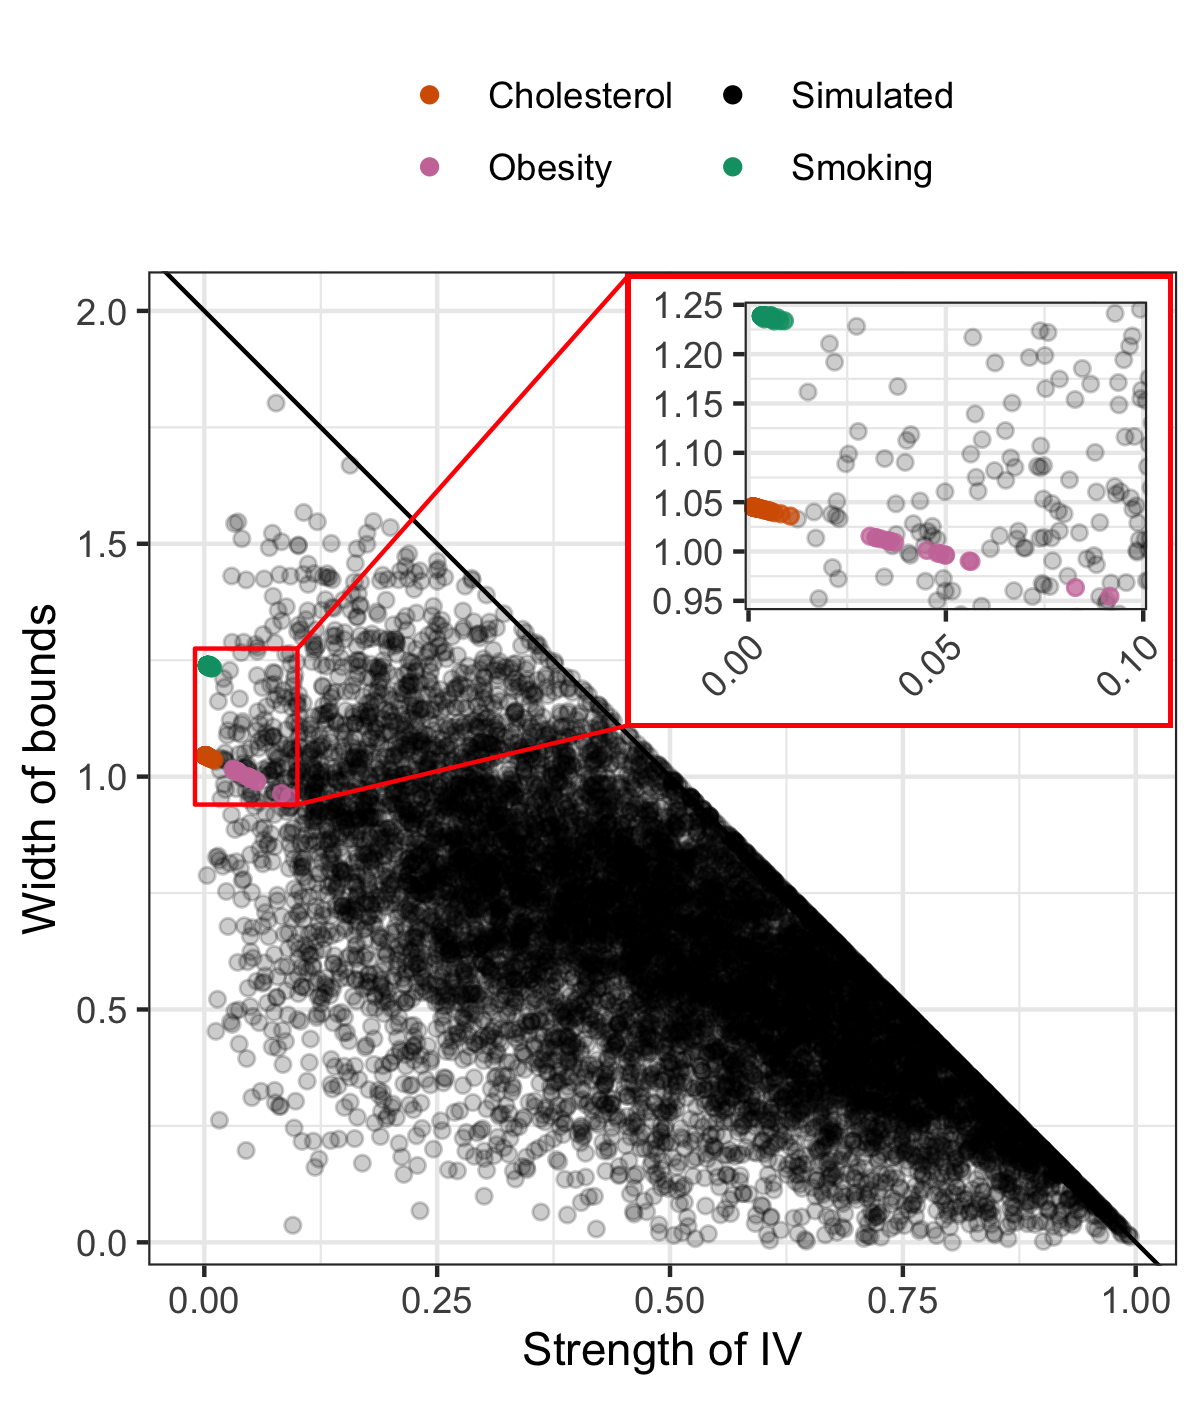
\includegraphics[width=\textwidth]{/Users/ralphtrane/Documents/RPackages_dev/ACEBounds/figures/bivariate_width_vs_strength_pip.png}
    \caption{Relationship between strength of an instrument (ST) and width of the IV bounds. Black line is the upper bound on the bound's width based on Theorem 1. Black dots indicate one of the 10,000 IV bounds. Colored dots indicate bounds from real data; see Section \ref{data-analysis} for details.}
    \label{fig:biv_width_vs_strength}
  \end{subfigure}%
  \hspace{0.15in}
  \begin{subfigure}[t]{0.48\textwidth}
    \centering
    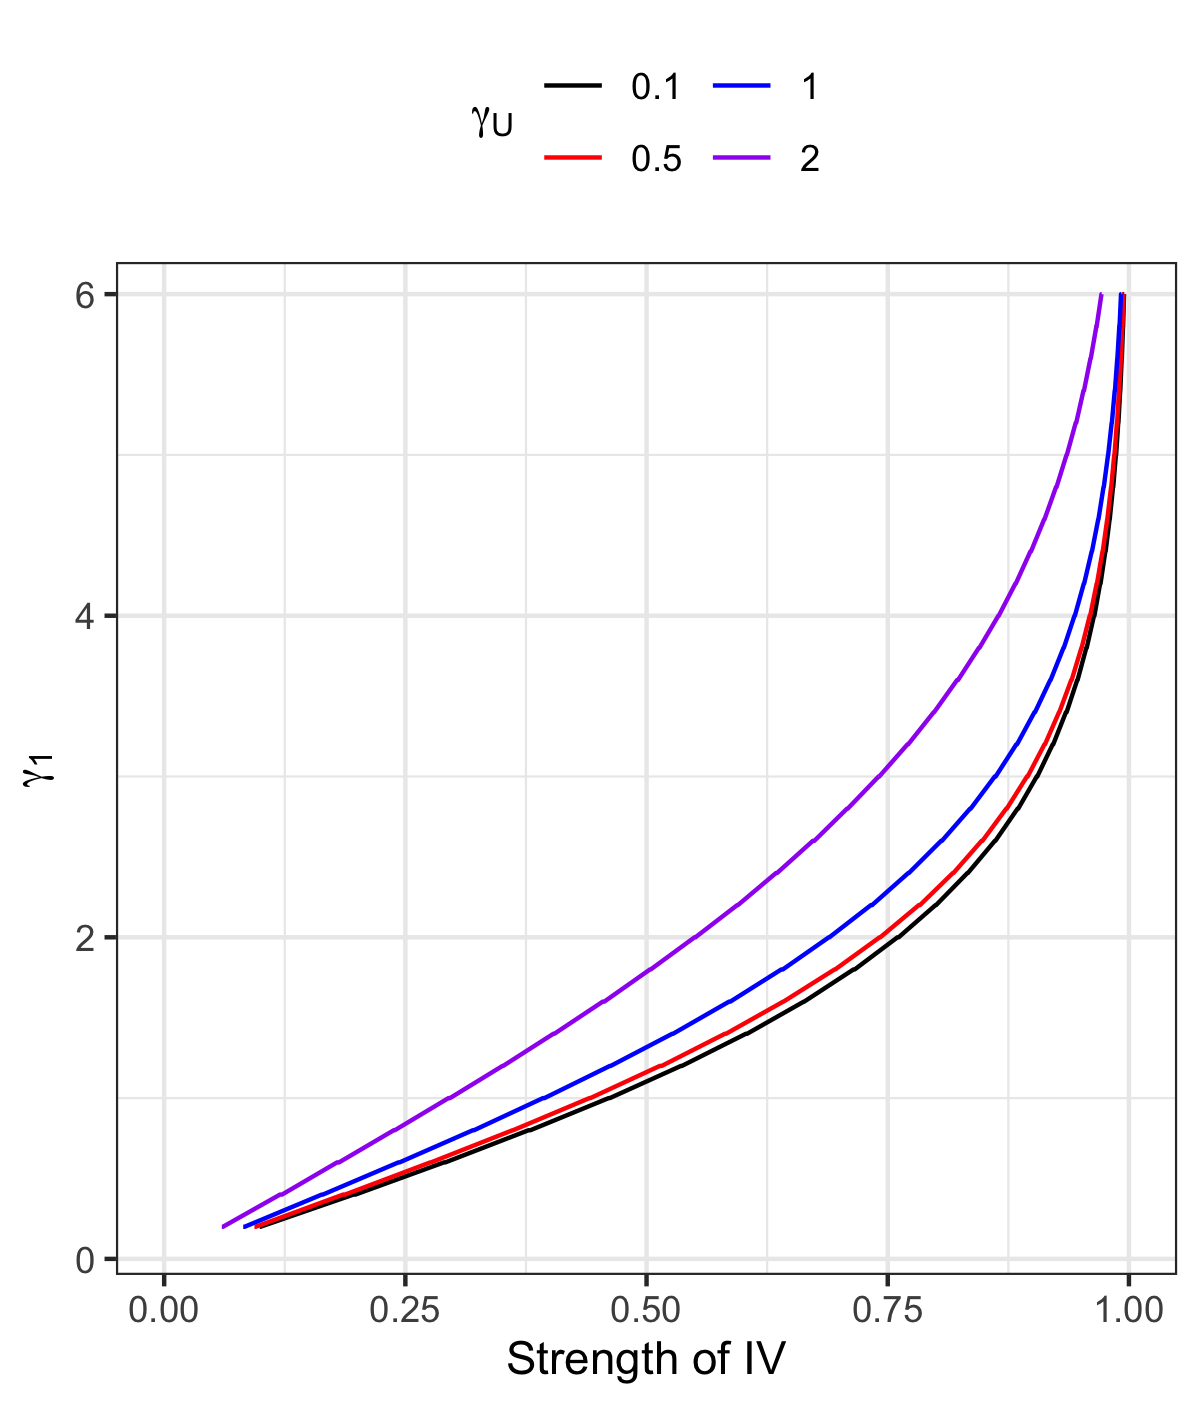
\includegraphics[width=\textwidth]{/Users/ralphtrane/Documents/RPackages_dev/ACEBounds/figures/MR_coefs_vs_strength.png}
    \caption{Coefficients from simple logistic regression model used to derive summary statistics and strength of instrument (ST).}
    \label{fig:coef_vs_strength}
  \end{subfigure}
  \caption{Illustration of the relationship between instrument strength, and width of bounds obtained from two-sample design and coefficients from logistic regression model.}
  \label{fig:biv_bounds_vs_strength}
\end{figure*}

For bounds with length less than \(1\), we study whether they can be informative about the direction of the exposure effect by asking what kind of summary statistic \(\gamma_1\) is needed in order for the two-sample IV bounds to exclude \(0\) for an anticipated effect size of the ATE. This question is akin to computing the power of bounds\%where instrument strength roughly stands for sample size but with population-level quantities. We reuse the same logistic model from above for the exposure and the outcome; see Appendix \ref{appendix-sim-results} for details. Figure \ref{fig:power_curves} shows the smallest \(\gamma_1\) needed to exclude \(0\) for different values of the ATE. Even for moderate effect sizes of 0.4, the corresponding \(\gamma_1\) must be around \(2\), a tall order for most GWAS summary statistics. Also, as the effect of unmeasured confounding increases via \(\gamma_U\), a larger \(\gamma_1\) is needed to exclude \(0\).

\begin{figure}[H]
  \centering
  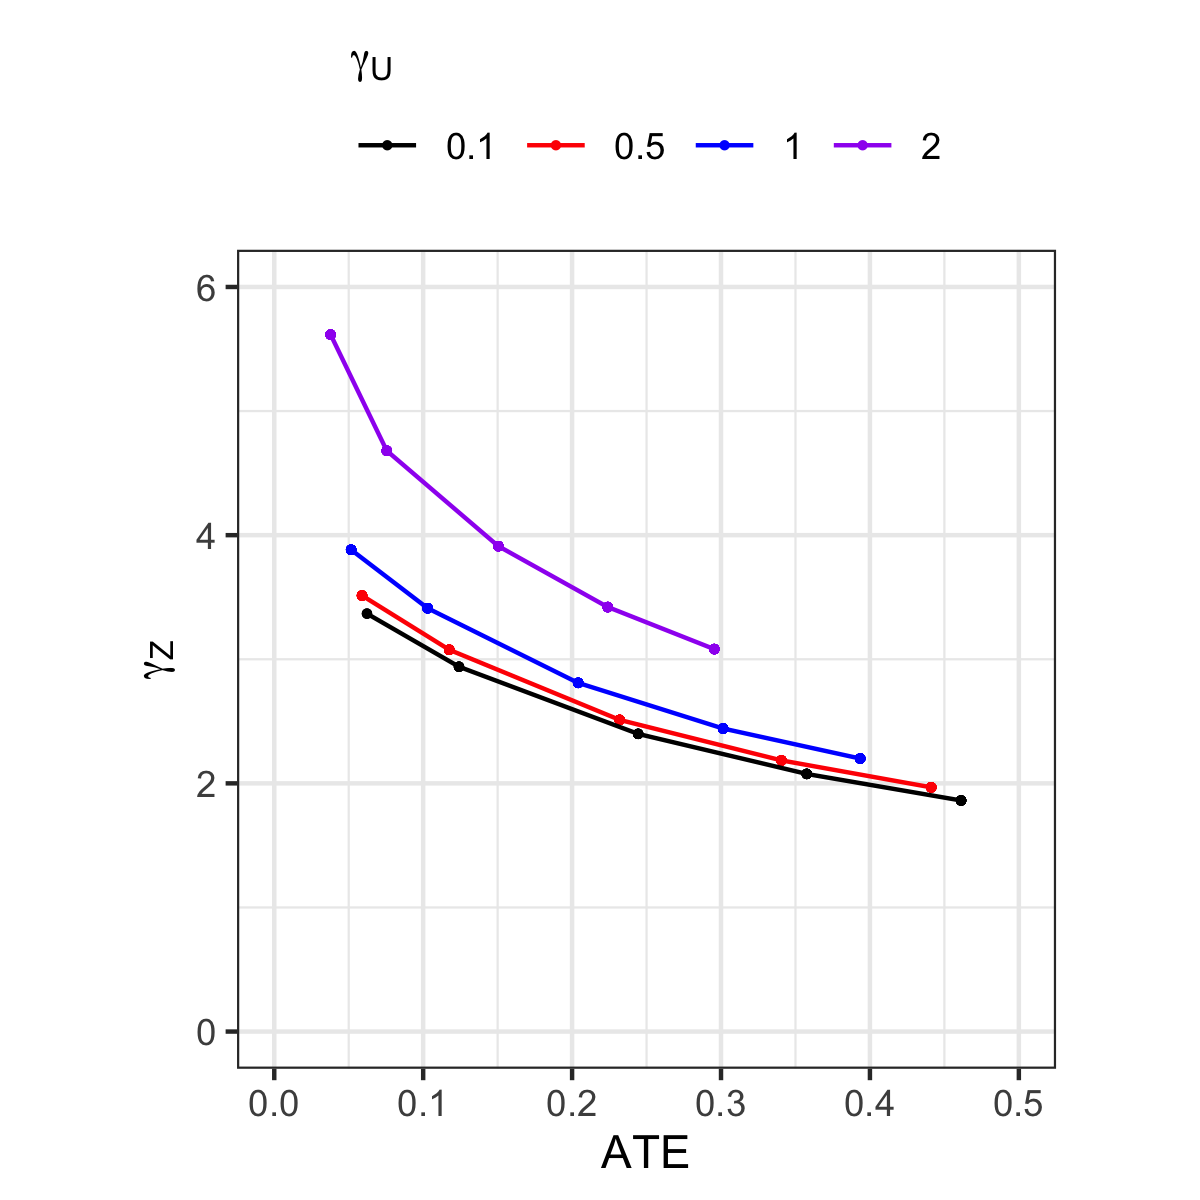
\includegraphics[width=0.99\textwidth]{/Users/ralphtrane/Documents/RPackages_dev/ACEBounds/figures/loess_power.png}
  \caption{The smallest $\gamma_1$ needed for a two-sample IV bound to exclude $0$.}
  \label{fig:power_curves}
\end{figure}

Overall, in the context of two-sample MR studies, an analysis based on bounds is unlikely to be informative, especially when most genetic instruments are weak. The bounds will often have length greater than \(1\) and rarely exclude \(0\) unless very strong genetic variants are used.

\hypertarget{would-multiple-instruments-help}{%
\subsection{Would Multiple Instruments Help?}\label{would-multiple-instruments-help}}

Based on the results above with a single instrument, a natural question from investigators is whether using multiple instruments can lead to more informative bounds for the ATE. For example, suppose we aggregate two-sample IV bounds across multiple instruments by taking intersections of individual IV bounds. This approach may be inferior to another alternative where we expand the levels of \(Z\) from \(0,1,2\) to accommodate multiple instruments \autocite{swanson_commentary_2017}, but has the benefit of being applicable to most two-sample MR studies. However, as we show in Appendix \ref{appendix-sim-results-multiple-IVs}, the strongest instrument essentially determines the length of the intersection bound because the individual bounds exhibit a nesting property. In short, using a bound based on the strong instrument provides the same amount of information about the ATE as the intersection of individual IV bounds from multiple instruments.

\hypertarget{charactering-the-loss-of-information-in-two-sample-mr-studies}{%
\section{Charactering the Loss of Information in Two-Sample MR Studies}\label{charactering-the-loss-of-information-in-two-sample-mr-studies}}

\label{quasi-bayesian}

As hinted in Theorem \ref{thm:upperBoundWidth}, the increase in the bound's length is an inevitable ``cost'' of using two-sample designs instead of one-sample designs. Indeed, the proof of the theorem shows that the loss of information can be directly attributed to the lack of information about the joint distribution \(P(X, Y | Z)\). Recognizing this, we obtain more informative bounds from two-sample MR by creating a plausible range of the joint distribution of the outcome and the exposure given the instrument \(Z\), \(P(X = x, Y = y | Z = z)\) based on the observed data from two-sample MR studies. Specifically, using \(P(X = x | Z = z)\) and \(P(Y = y | Z = z)\), and a uniform prior on unknown quantities \(\text{Cov}(X = x, Y = y| Z = z)\) that make up \(P(X,Y | Z)\) and satisfy IV assumptions, we compute \(P(X = x, Y = y | Z = z)\) and its corresponding one-sample IV bounds of \textcite{balke_bounds_1997} and \textcite{richardson_ace_2014}; see Appendix \ref{appendix-quasi-bayesian-details} for details and also its connection to empirical Bayesian frameworks. If a large number of the one-sample IV bounds obtained do not cover zero, then there is some evidence for a non-zero exposure effect and a one-sample design may yield informative bounds on the ATE. However, if a large number of the one-sample IV bounds cover zero, there is little hope of obtaining information about the ATE from bound-based approaches even if we one-sample design; in other words, the one-sample IV bounds are likely as conservative as the two-sample IV bounds.

Table \ref{tab:subset_plot_summaries} presents nine different sets of values of the marginal distributions \(P(Y | Z)\) and \(P(X | Z)\) that investigators could theoretically obtain from hypothetical two-sample MR studies. Figure \ref{fig:trivariate_bounds} shows the one-sample IV bounds from the procedure we illustrated above.

\begin{table}[H]
  \center
  \caption{Values of $P(X = 1 | Z = z)$ and $P(Y = 1 | Z = z)$ used to illustrate our approach. For each cell (e.g. row A, column 1), we have $\{P(X = 1 | Z = 0), P(X = 1 | Z = 1), P(X = 1 | Z = 2)\}$ on the first row and $\{P(Y = 1 | Z = 0), P(Y = 1 | Z = 1), P(Y = 1 | Z = 2)\}$ on the second row.}
  \label{tab:subset_plot_summaries}
  
\begin{tabular}{llll}
\toprule
  & Column 1 & Column 2 & Column 3\\
\midrule
Row A & \makecell[l]{\{0.125, 0.399, 0.080\}\\\{0.699, 0.840, 0.742\}} & \makecell[c]{\{0.244, 0.275, 0.185\}\\\{0.238, 0.089, 0.146\}} & \makecell[r]{\{0.603, 0.469, 0.310\}\\\{0.638, 0.346, 0.719\}}\\
Row B & \makecell[l]{\{0.886, 0.968, 0.874\}\\\{0.805, 0.822, 0.951\}} & \makecell[c]{\{0.139, 0.441, 0.334\}\\\{0.179, 0.359, 0.559\}} & \makecell[r]{\{0.901, 0.909, 0.935\}\\\{0.821, 0.810, 0.905\}}\\
Row C & \makecell[l]{\{0.175, 0.079, 0.365\}\\\{0.599, 0.358, 0.087\}} & \makecell[c]{\{0.493, 0.911, 0.085\}\\\{0.360, 0.480, 0.441\}} & \makecell[r]{\{0.434, 0.045, 0.733\}\\\{0.747, 0.370, 0.169\}}\\
\bottomrule
\end{tabular}


\end{table}

\begin{figure}[H]
  \center
  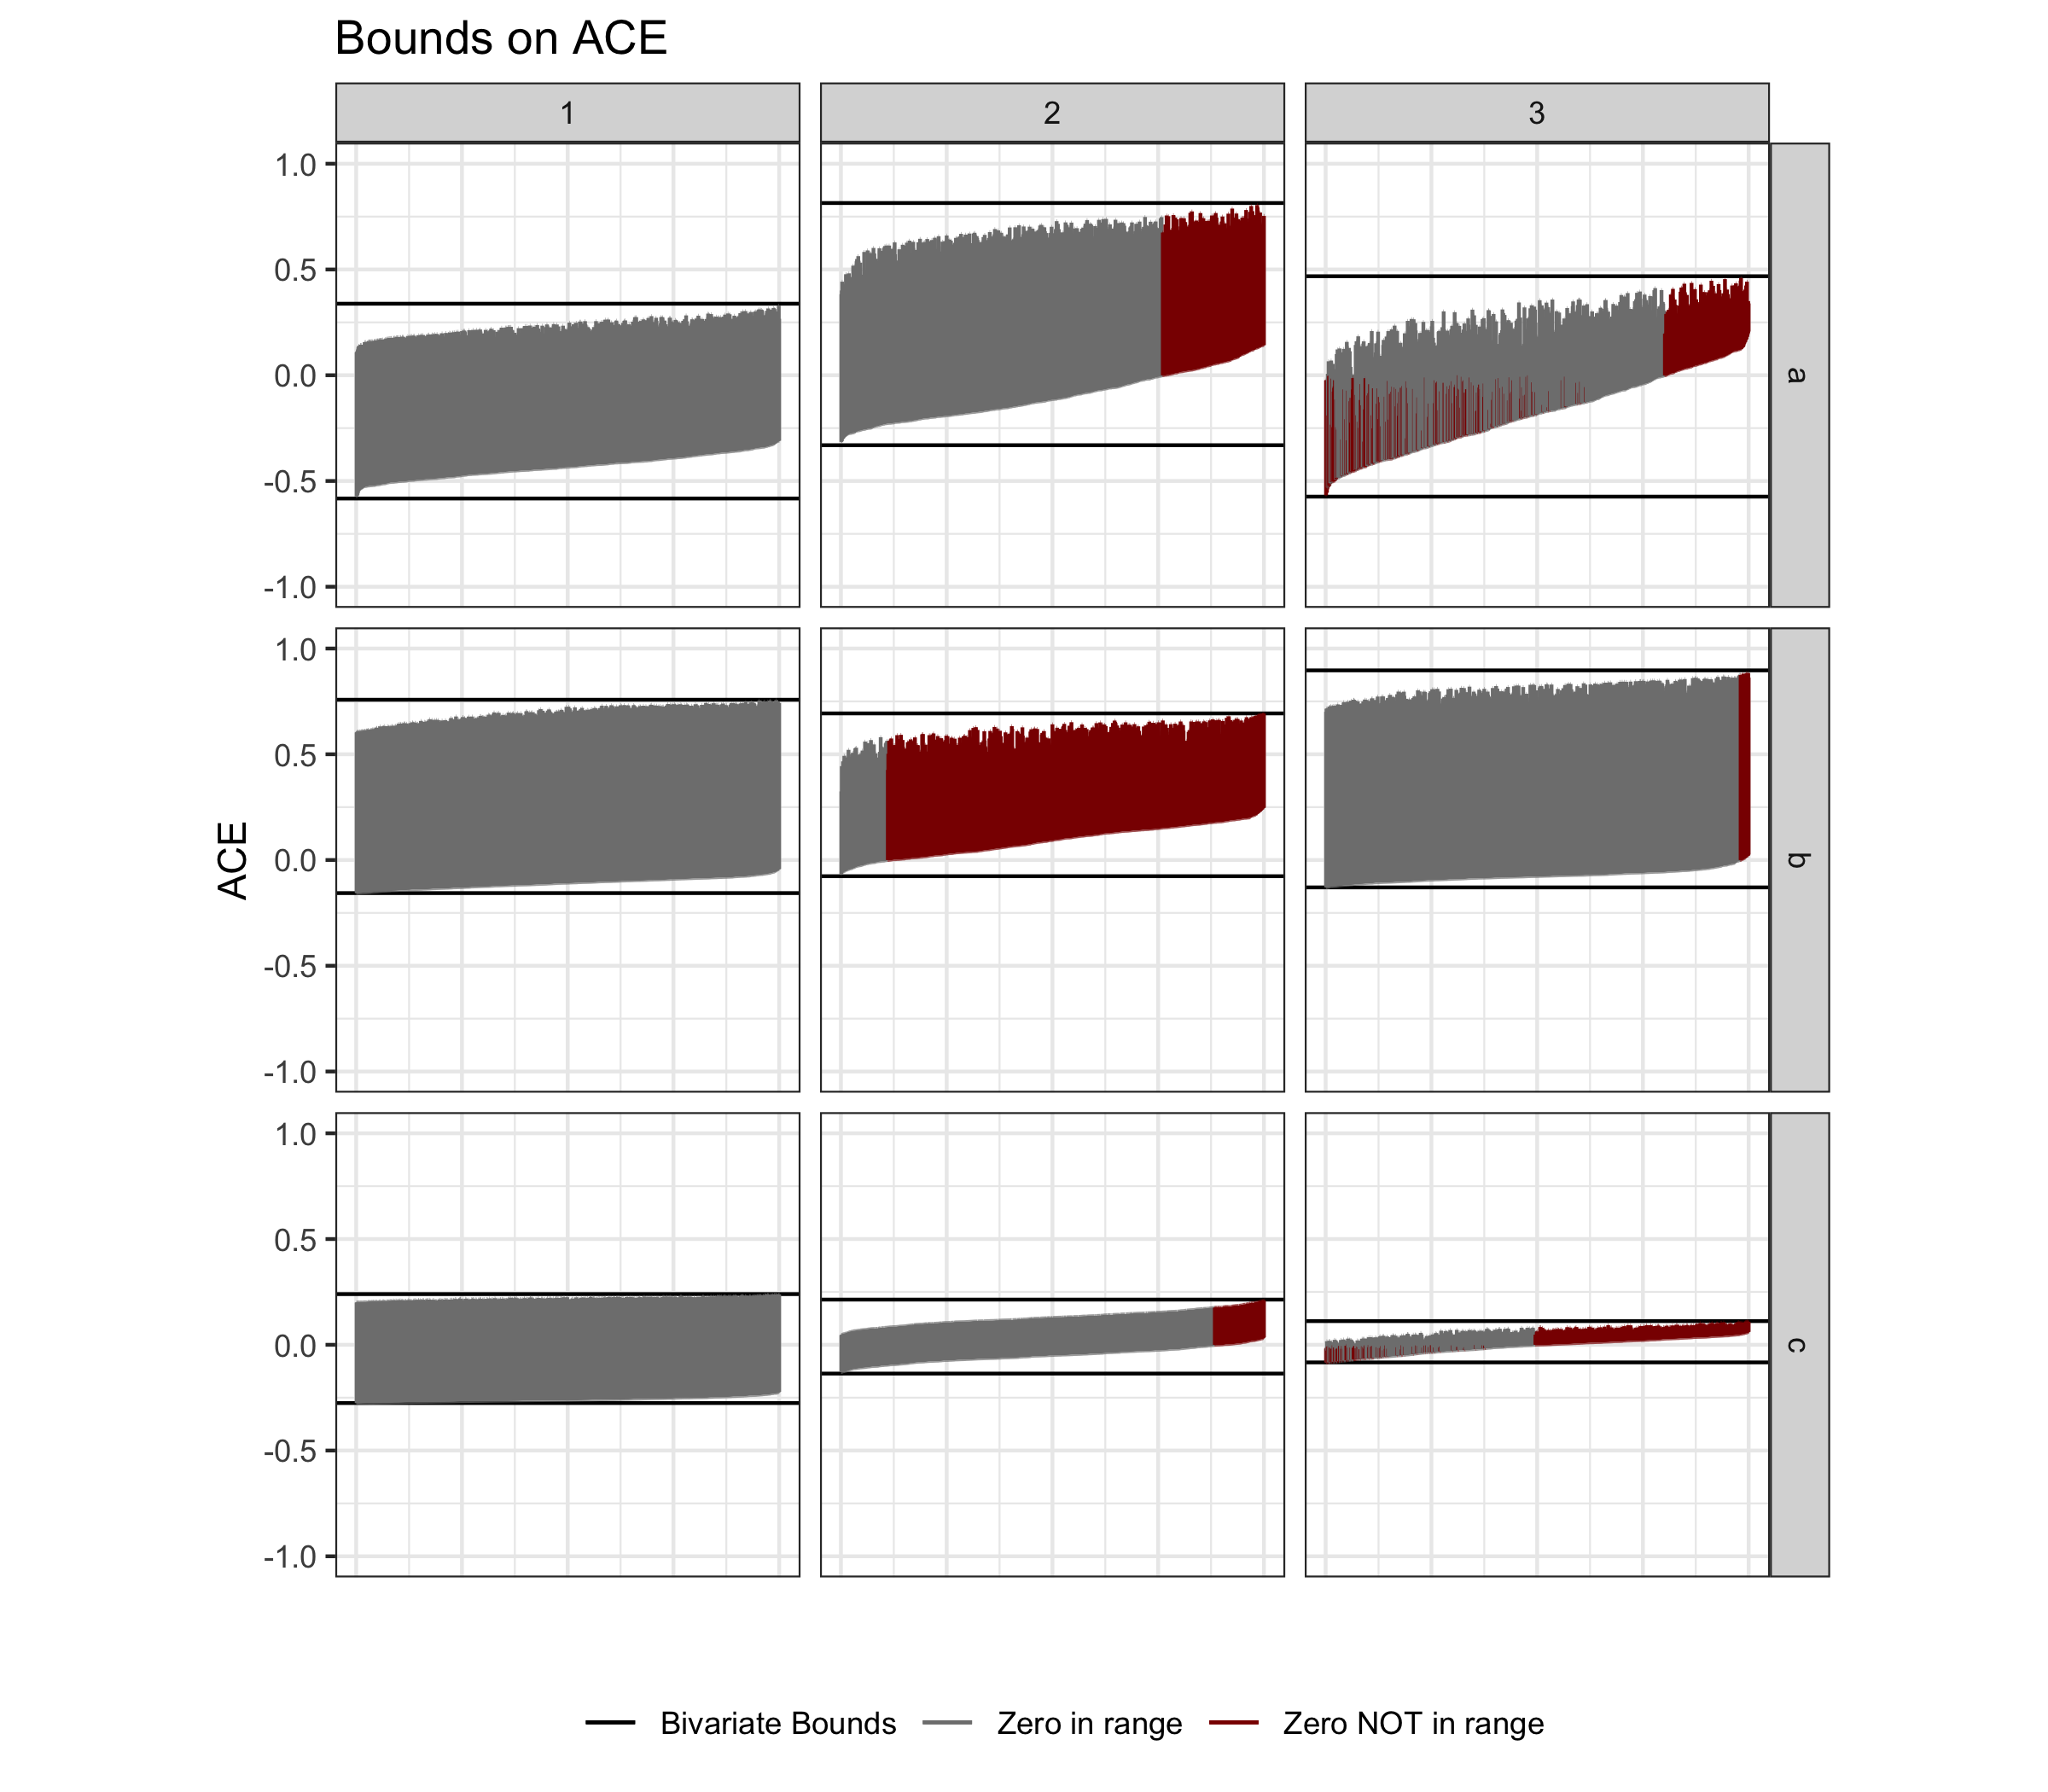
\includegraphics[width=\linewidth]{/Users/ralphtrane/Documents/RPackages_dev/ACEBounds/figures/trivariate_bounds_subset_plot.png}
  \caption{One-sample bounds (solid lines) and two-sample bounds (dotted lines). Red color represents one-sample bounds that do not cover zero and gray color represents one-sample bounds that do cover zero.}
  \label{fig:trivariate_bounds}
\end{figure}

Row A of Figure \ref{fig:trivariate_bounds} shows three scenarios where the two-sample bounds are all centered close to zero with similar widths. But, the conclusions from the one-sample bound analysis are rather different. Column 1 shows no one-sample bounds would allow us to determine the presence of a non-zero exposure effect. Column 2 indicates that about 24\% of the one-sample IV bounds does not contain \(0\) while for column 3 that number is approximately 36.8\%\%.

Row B illustrates three scenarios where the two-sample bounds are centered well above zero and have large widths. We see one case where we have no hope of determining direction of the ATE from the one-sample bounds (column 1), one case where we are most likely to determine the ATE's direction (column 2), and one case where we are unlikely to determine the ATE' direction (column 3).

Row C is similar to row A in that all the two-sample bounds are centered around 0, but the widths of the two-sample bounds are narrow. The three columns indicate similar conclusions as row A, showing that even with rather narrow two-sample bounds centered around 0, the one-sample bounds may still reveal some information about presence as well as the direction of the exposure effect.

Overall, our results above show that some two-sample MR studies could potentially reveal something useful about the ATE had we used a one-sample design. Nevertheless, we mention a word of caution when interpreting the results above, especially concerning the flat prior on the covariances. For example, a scenario like the one resulting in the bounds presented in row B, column 2 only provides honest information about the one-sample bounds if our prior on \(\text{Cov}(X,Y|Z)\) is correctly specified. If the prior is mis-specified whereby most one-sample bounds cover negative values of the ATE, a negative value of the ATE is possible. But in this case, if the ATE is in fact negative, our method does rule out the possibility of one-sample bounds being able to ascertain this because all one-sample bounds covering a negative ATE also covers \(0\).

\hypertarget{results}{%
\section{\texorpdfstring{Results \label{data-analysis}}{Results }}\label{results}}

We demonstrate our findings about the behavior of two-sample IV bounds on two real MR studies. Our first study examines the effect of smoking on lung cancer and our second study examines the effect of self-reported high cholesterol on incidence of heart attack. The effect of smoking on lung cancer is known to be strong and positive. Also, while the exact mechanism between high cholesterol and heart disease is still being discussed \autocite{holmes_mendelian_2015,richardson_evaluating_2020}, some meta-analyses of randomized clinical trials of the effect of cholesterol-lowering medication suggest a strong causal relationship \autocite{20051267,cholesterol_treatment_trialists_ctt_collaborators_effects_2012}. In both cases, we assess what conclusions are attainable based on bound-based approaches in settings where the causal effects are known to be strong and positive.

The study data were obtained from the UK Biobank data stored in the Integrative Epidemiology Unit (IEU) GWAS database. Specifically, data on smoking was obtained from the data entry ID ukb-d-20116\_0, data on lung cancer was from data entry ID ukb-d-40001\_C349, data on cholesterol was from data entry ID ukb-a-108, and data on heart attack was from data entry ID ukb-a-434. We use the \texttt{TwoSampleMR} R package \autocite{mrbase} with the recommended defaults to extract and clean the data.

The study data were obtained from the UK Biobank data stored in the Integrative Epidemiology Unit (IEU) GWAS database. Specifically, data on smoking was obtained from the data entry ID ukb-d-20116\_0, data on lung cancer was from data entry ID ukb-d-40001\_C349, data on cholesterol was from data entry ID ukb-a-108, and data on heart attack was from data entry ID ukb-a-434. We use the \texttt{TwoSampleMR} R package \autocite{mrbase} with the recommended defaults to extract and clean the data.

For the effect of smoking on lung cancer, we used 84 genetic instruments, and for the effect of cholesterol on heart attack, we used 54 genetic instruments. The average instrument strengths were 0.0042 (range: 0.0032 to 0.0091) for smoking and 0.0005 (range: 0.0002 to 0.0022) for cholesterol; these values are much smaller than the ST \(= 0.5\) needed to guarantee narrow bounds. As such, the two-sample bounds in Figure \ref{fig:ind_bounds} are rather wide; all of them have width greater than 1 and they convey no information about the causal effects of interest. Additionally, using our method from Section \ref{quasi-bayesian}, the direction of the ATE may be difficult to determine had we had one-sample IV bounds; see Figure \ref{fig:tri_bounds} \textcolor{red}{include this figure}. Appendix \ref{more-details-data-application-appendix} contains additional analysis, notably demonstrating that aggregating bounds through intersections are also non-informative.

Overall, while nonparametric bounds allow us to not make parametric assumptions frequent in two-sample MR analyses, they may be too conservative and provide little, if any, information about the exposure effects, even if the exposure effect is known to be positive and strong. Additionally, since many MR studies involve weak instruments, we believe bound-based approaches will likely have limited practical value to uncover causal effects.

\hypertarget{discussion}{%
\section{\texorpdfstring{Discussion \label{conclusion-and-practical-considerations}}{Discussion }}\label{discussion}}

Nonparametric bounds are without a doubt an attractive concept. With a minimal set of assumptions, they let investigators obtain bounds on the average treatment effect. However, as we have seen above, in typical MR studies with two-sample summary data, a bound-based analysis may generally uninformative for two reasons. First, while IV bounds in one-sample settings have length always being less than 1, in two-sample settings, this is not always the case. Second, many genetic variants in MR studies are weakly associated with the exposure to lead to bounds with length less than \(1\) or bounds that exclude \(0\). Indeed, our two real data examples showed that despite having strong causal effects, a bound-based analysis was unable to detect this effect.

We also outlined an approach to roughly quantify the information loss going from two-sample designs to one-sample designs and to assess the range of conclusions that can be drawn from bound-based approaches if we had one-sample data. We demonstrate our method to a few different settings of two-sample data and showed the range conclusions that can be drawn about the ATE.

What do our results suggest for bound-based analysis in two-sample MR settings in practice? Overall, our general recommendation is that unless investigators have a very strong instrument, ideally exceeding \(ST >0.5\), bounds will unlikely be useful as a nonparametric analysis of the ATE. Also, aggregating information from many instruments through simple intersections will only be as good as using a single strong instrument. But, there may be few limited, but meaningful use cases for bounds in two-sample MR studies. First when one has prior knowledge about the direction of the effect, but wish to get a better sense of the magnitude, nonparametric bounds can provide an upper limit on this magnitude. This is especially useful in cases where the exposure is known to cause harm or benefit, for example in our smoking lung cancer example where the direction of the effect of smoking on lung cancer is well known and an upper bound on this effect would tell investigators about the maximum possible effect that smoking could have on increasing the incidence of lung cancer. Second, two-sample IV bounds can be used to check estimates from parametric methods to see if they lie inside of the bounds; if the estimates lie outside of the bounds, then the parametric models underlying the estimates are likely mis-specified.

\newpage

\hypertarget{appendix-appendix}{%
\appendix}


\hypertarget{logistic-models}{%
\section{\texorpdfstring{Logistic Models \label{appendix-logistic-models}}{Logistic Models }}\label{logistic-models}}

When a GWAS is run to find associations between genetic markers and a binary trait, the logitisc regression model is often used. For this particular reason, we use the logistic model in our monte carlo integrations to characterize the behavior of the non-parametric bounds from two-sample data.

Specifically, we assume that \(P(Z = 0) = P(Z = 2) = 0.25\) and \(P(Z = 1) = 0.5\), and a value of an unmeasured confounder \(U\) from the standard normal. We assume the exposure \(X\) is binary with \(\text{logit}(P(X = 1 | Z_1 = z_1, ..., Z_p = z_p, U = u)) = \gamma_0 + \sum_i \gamma_i z_i + \gamma_U u\), where \(\text{logit}(a) = \frac{1}{1+\exp(a)}\) and \(\gamma_i\) corresponds to the estimand of the regression estimate one would obtain from GWAS studying the relationship between the genetic variant and the exposure. This model has been used in MR studies by \textcite{burgess_sample_2014} and \textcite{burgess_improving_2012} so that every instrument estimates the same exposure effect. Similarly, we assume that the outcome \(Y\) is binary with \(P(Y = 1 | X = x, U = u) = \text{logit}(\beta_0 + \beta_X \cdot x + \beta_U \cdot u)\), which we use to compute the true ATE.

\hypertarget{bounds-on-average-treatment-effect}{%
\section{Bounds on Average Treatment Effect}\label{bounds-on-average-treatment-effect}}

We briefly review the method presented by \textcite{ramsahai_causal_2012} to bound the average treatment effect using two-sample summary data. Let \(\vec{\tau}^* = \Big(P(Y = 1 | X = 0, U), P(Y = 1 | X = 1, U), P(X = 1 | Z = 0, U), ..., P(X = 1 | Z = k-1, U)\Big) \in [0,1]^{2+k}\) and \(\vec{v}^* = \Big(P(Y = 0 | Z = 0, U), ..., P(Y = 1 | Z = k-1, U), P(X = 0 | Z = 0, U), ..., P(X = 1 | Z = k-1, U), \alpha^*\Big)\) where

\[
\begin{aligned}
\alpha^* &= P(Y = 1 | X = 1, U) - P(Y = 1 | X = 0, U).
\end{aligned}
\]

Since \(U \perp Z\), \(E_U[P(X = x | Z = z, U)] = P(X = x | Z = z)\) and \(E_U[P(Y = y | Z = z, U)] = P(Y = y | Z = z)\). Let \(\vec{v} = E_U[\vec{v}^*] = \Big(P(Y = 0 | Z = 0), ..., P(Y = 1 | Z = k-1), P(X = 0 | Z = 0), ..., P(X = 1 | Z = k-1), \alpha \Big)\), where

\[
\begin{aligned}
\alpha &= E_U[P(Y = 1 | X = 1, U) - P(Y = 1 | X = 0, U)] \\
       &= E[Y^1] - E[Y^0] = \text{ATE}.
\end{aligned}
\]

Note that while \(\vec{\tau}^*\) and \(\vec{v}^*\) are both entirely unobervable, \(\vec{v}\) consists of \(k\) observable values, and one unobservable value, the ATE.

By the exclusion restriction, we have

\[
P(X = x, Y = y | Z = z, U) = P(Y = 1 | X = x, U) P(X = x | Z = z, U),
\]

which means we can define a mapping \(f:[0,1]^{2+k} \mapsto \mathcal{V}\) such that \(f(\vec{\tau}^*) = \vec{v^*}\) as

\[
f(y_0, y_1, x_0, x_1, ..., x_{k-1}) =
  \begin{pmatrix}
    (1-y_0)\cdot(1-x_0) + (1 - y_1)\cdot x_0 \\
    y_0\cdot (1-x_0) + y_1\cdot x_0 \\
    \vdots \\
    (1-y_0)\cdot(1-x_{k-1}) + (1 - y_1)\cdot x_{k-1} \\
    y_0\cdot (1-x_{k-1}) + y_1\cdot x_{k-1}
  \end{pmatrix} \label{eq:f}
\]

We define \(\mathcal{V} = f([0,1]^{2+k})\).

Since \(\vec{v} = E_U[\vec{v}^*]\), \(\vec{v}\) must be a convex combination of \(\vec{v}^*\). Let \(\mathcal{H}\) be the convex hull of \(\mathcal{V}\). Then \(\vec{v}\) will be in \(\mathcal{H}\).

Now, let \(\hat{\mathcal{T}}\) be the set of extreme vertices of \([0,1]^{2+k}\), \(\hat{\mathcal{V}} = f(\hat{\mathcal{T}})\), and \(\hat{\mathcal{H}}\) be the convex hull of \(\hat{\mathcal{V}}\). By Theorem 1 in Appendix B of \textcite{ramsahai_causal_2012}, \(\mathcal{H} = \mathcal{\hat{H}}\). This means that \(\vec{v} \in \mathcal{\hat{H}}\). Utilizing a program such as Polymake, we can describe \(\mathcal{H}\) with a set of inequalities, which give us constraints that \(\vec{v}\) must satisfy.

This means that we can obtain inequalities that the components of \(\vec{v}\) must satisfy by describing the extreme vertices of \([0,1]^{2+k}\), map them to \(\mathcal{V}\) using the relatively simple function \(f\), and then use polymake to find inequalities that characterize the convex hull of \(f([0,1])^{2+k}\). This gives us a set of inequalities involving the components of \(\vec{v}\). Some of these will be verifiable, as they will not include the only unobservable quantity \(\alpha\). Others will not be verifiable, but will allow us to obtain bounds on the unobservable quantity \(\alpha\) using the observable entries of \(\vec{v}\).

Following the approach from Ramsahai (2012) as outlined above, we obtain bounds on the average treatment effect from the quantities \(P(X = 1 | Z = z)\) and \(P(Y = 1 | Z = z)\), \(z = 0,1,2\). To do so, we first write down the most extreme values of each of \(P(Y = 1 | X = x, U)\) and \(P(X = x | Z = z, U)\) for all \(x=0,1\), \(z=0,1,2\). Since these are probabilities, the extreme values are \(0\) and \(1\).

\begin{longtable}[]{@{}
  >{\centering\arraybackslash}p{(\columnwidth - 8\tabcolsep) * \real{0.12}}
  >{\centering\arraybackslash}p{(\columnwidth - 8\tabcolsep) * \real{0.12}}
  >{\centering\arraybackslash}p{(\columnwidth - 8\tabcolsep) * \real{0.12}}
  >{\centering\arraybackslash}p{(\columnwidth - 8\tabcolsep) * \real{0.12}}
  >{\centering\arraybackslash}p{(\columnwidth - 8\tabcolsep) * \real{0.12}}@{}}
\caption{Most extreme values of \(P(Y = 1 | X = x, U)\) and \(P(X = 1 | Z = z, U)\). Here, PY1XxU = \(P(Y = 1 | X = x, U)\) and PX1ZzU = \(P(X = 1 | Z = z, U)\).}\tabularnewline
\toprule
PY1X0U & PY1X1U & PY1Z0U & PX1Z1U & PX1Z2U \\ \addlinespace
\midrule
\endfirsthead
\toprule
PY1X0U & PY1X1U & PY1Z0U & PX1Z1U & PX1Z2U \\ \addlinespace
\midrule
\endhead
0 & 0 & 0 & 0 & 0 \\ \addlinespace
0 & 0 & 0 & 0 & 1 \\ \addlinespace
0 & 0 & 0 & 1 & 0 \\ \addlinespace
0 & 0 & 0 & 1 & 1 \\ \addlinespace
0 & 0 & 1 & 0 & 0 \\ \addlinespace
0 & 0 & 1 & 0 & 1 \\ \addlinespace
0 & 0 & 1 & 1 & 0 \\ \addlinespace
0 & 0 & 1 & 1 & 1 \\ \addlinespace
0 & 1 & 0 & 0 & 0 \\ \addlinespace
0 & 1 & 0 & 0 & 1 \\ \addlinespace
0 & 1 & 0 & 1 & 0 \\ \addlinespace
0 & 1 & 0 & 1 & 1 \\ \addlinespace
0 & 1 & 1 & 0 & 0 \\ \addlinespace
0 & 1 & 1 & 0 & 1 \\ \addlinespace
0 & 1 & 1 & 1 & 0 \\ \addlinespace
0 & 1 & 1 & 1 & 1 \\ \addlinespace
1 & 0 & 0 & 0 & 0 \\ \addlinespace
1 & 0 & 0 & 0 & 1 \\ \addlinespace
1 & 0 & 0 & 1 & 0 \\ \addlinespace
1 & 0 & 0 & 1 & 1 \\ \addlinespace
1 & 0 & 1 & 0 & 0 \\ \addlinespace
1 & 0 & 1 & 0 & 1 \\ \addlinespace
1 & 0 & 1 & 1 & 0 \\ \addlinespace
1 & 0 & 1 & 1 & 1 \\ \addlinespace
1 & 1 & 0 & 0 & 0 \\ \addlinespace
1 & 1 & 0 & 0 & 1 \\ \addlinespace
1 & 1 & 0 & 1 & 0 \\ \addlinespace
1 & 1 & 0 & 1 & 1 \\ \addlinespace
1 & 1 & 1 & 0 & 0 \\ \addlinespace
1 & 1 & 1 & 0 & 1 \\ \addlinespace
1 & 1 & 1 & 1 & 0 \\ \addlinespace
1 & 1 & 1 & 1 & 1 \\ \addlinespace
\bottomrule
\end{longtable}

By applying the function \(f\), as presented in \eqref{eq:f}, to each row, we get the most extreme vertices of \(P(X = x | Z = z, U)\) and \(P(Y = y | Z = z, U)\) for all \(x=0,1,\ y=0,1\) and \(z=0,1,2\).

\begin{longtable}[]{@{}
  >{\centering\arraybackslash}p{(\columnwidth - 24\tabcolsep) * \real{0.07}}
  >{\centering\arraybackslash}p{(\columnwidth - 24\tabcolsep) * \real{0.07}}
  >{\centering\arraybackslash}p{(\columnwidth - 24\tabcolsep) * \real{0.07}}
  >{\centering\arraybackslash}p{(\columnwidth - 24\tabcolsep) * \real{0.07}}
  >{\centering\arraybackslash}p{(\columnwidth - 24\tabcolsep) * \real{0.07}}
  >{\centering\arraybackslash}p{(\columnwidth - 24\tabcolsep) * \real{0.07}}
  >{\centering\arraybackslash}p{(\columnwidth - 24\tabcolsep) * \real{0.07}}
  >{\centering\arraybackslash}p{(\columnwidth - 24\tabcolsep) * \real{0.07}}
  >{\centering\arraybackslash}p{(\columnwidth - 24\tabcolsep) * \real{0.07}}
  >{\centering\arraybackslash}p{(\columnwidth - 24\tabcolsep) * \real{0.07}}
  >{\centering\arraybackslash}p{(\columnwidth - 24\tabcolsep) * \real{0.07}}
  >{\centering\arraybackslash}p{(\columnwidth - 24\tabcolsep) * \real{0.07}}
  >{\centering\arraybackslash}p{(\columnwidth - 24\tabcolsep) * \real{0.10}}@{}}
\caption{Most extreme values of \(P(Y = y | Z = z)\) and \(P(X = x | Z = z)\). Here, PYyZz = \(P(Y = y | Z = z)\), PXxZz = \(P(X = x | Z = z)\), and \(\alpha = P(Y = 1 | X = 1,U) - P(Y = 1 | X = 0,U)\).\label{tab:vertices}}\tabularnewline
\toprule
PY0Z0 & PY0Z1 & PY0Z2 & PY1Z0 & PY1Z1 & PY1Z2 & PX0Z0 & PX0Z1 & PX0Z2 & PX1Z0 & PX1Z1 & PX1Z2 & \(\alpha\) \\ \addlinespace
\midrule
\endfirsthead
\toprule
PY0Z0 & PY0Z1 & PY0Z2 & PY1Z0 & PY1Z1 & PY1Z2 & PX0Z0 & PX0Z1 & PX0Z2 & PX1Z0 & PX1Z1 & PX1Z2 & \(\alpha\) \\ \addlinespace
\midrule
\endhead
1 & 1 & 1 & 0 & 0 & 0 & 1 & 1 & 1 & 0 & 0 & 0 & 0 \\ \addlinespace
0 & 0 & 0 & 1 & 1 & 1 & 1 & 1 & 1 & 0 & 0 & 0 & -1 \\ \addlinespace
1 & 1 & 1 & 0 & 0 & 0 & 1 & 1 & 1 & 0 & 0 & 0 & 1 \\ \addlinespace
0 & 0 & 0 & 1 & 1 & 1 & 1 & 1 & 1 & 0 & 0 & 0 & 0 \\ \addlinespace
1 & 1 & 1 & 0 & 0 & 0 & 0 & 1 & 1 & 1 & 0 & 0 & 0 \\ \addlinespace
1 & 0 & 0 & 0 & 1 & 1 & 0 & 1 & 1 & 1 & 0 & 0 & -1 \\ \addlinespace
0 & 1 & 1 & 1 & 0 & 0 & 0 & 1 & 1 & 1 & 0 & 0 & 1 \\ \addlinespace
0 & 0 & 0 & 1 & 1 & 1 & 0 & 1 & 1 & 1 & 0 & 0 & 0 \\ \addlinespace
1 & 1 & 1 & 0 & 0 & 0 & 1 & 0 & 1 & 0 & 1 & 0 & 0 \\ \addlinespace
0 & 1 & 0 & 1 & 0 & 1 & 1 & 0 & 1 & 0 & 1 & 0 & -1 \\ \addlinespace
1 & 0 & 1 & 0 & 1 & 0 & 1 & 0 & 1 & 0 & 1 & 0 & 1 \\ \addlinespace
0 & 0 & 0 & 1 & 1 & 1 & 1 & 0 & 1 & 0 & 1 & 0 & 0 \\ \addlinespace
1 & 1 & 1 & 0 & 0 & 0 & 0 & 0 & 1 & 1 & 1 & 0 & 0 \\ \addlinespace
1 & 1 & 0 & 0 & 0 & 1 & 0 & 0 & 1 & 1 & 1 & 0 & -1 \\ \addlinespace
0 & 0 & 1 & 1 & 1 & 0 & 0 & 0 & 1 & 1 & 1 & 0 & 1 \\ \addlinespace
0 & 0 & 0 & 1 & 1 & 1 & 0 & 0 & 1 & 1 & 1 & 0 & 0 \\ \addlinespace
1 & 1 & 1 & 0 & 0 & 0 & 1 & 1 & 0 & 0 & 0 & 1 & 0 \\ \addlinespace
0 & 0 & 1 & 1 & 1 & 0 & 1 & 1 & 0 & 0 & 0 & 1 & -1 \\ \addlinespace
1 & 1 & 0 & 0 & 0 & 1 & 1 & 1 & 0 & 0 & 0 & 1 & 1 \\ \addlinespace
0 & 0 & 0 & 1 & 1 & 1 & 1 & 1 & 0 & 0 & 0 & 1 & 0 \\ \addlinespace
1 & 1 & 1 & 0 & 0 & 0 & 0 & 1 & 0 & 1 & 0 & 1 & 0 \\ \addlinespace
1 & 0 & 1 & 0 & 1 & 0 & 0 & 1 & 0 & 1 & 0 & 1 & -1 \\ \addlinespace
0 & 1 & 0 & 1 & 0 & 1 & 0 & 1 & 0 & 1 & 0 & 1 & 1 \\ \addlinespace
0 & 0 & 0 & 1 & 1 & 1 & 0 & 1 & 0 & 1 & 0 & 1 & 0 \\ \addlinespace
1 & 1 & 1 & 0 & 0 & 0 & 1 & 0 & 0 & 0 & 1 & 1 & 0 \\ \addlinespace
0 & 1 & 1 & 1 & 0 & 0 & 1 & 0 & 0 & 0 & 1 & 1 & -1 \\ \addlinespace
1 & 0 & 0 & 0 & 1 & 1 & 1 & 0 & 0 & 0 & 1 & 1 & 1 \\ \addlinespace
0 & 0 & 0 & 1 & 1 & 1 & 1 & 0 & 0 & 0 & 1 & 1 & 0 \\ \addlinespace
1 & 1 & 1 & 0 & 0 & 0 & 0 & 0 & 0 & 1 & 1 & 1 & 0 \\ \addlinespace
1 & 1 & 1 & 0 & 0 & 0 & 0 & 0 & 0 & 1 & 1 & 1 & -1 \\ \addlinespace
0 & 0 & 0 & 1 & 1 & 1 & 0 & 0 & 0 & 1 & 1 & 1 & 1 \\ \addlinespace
0 & 0 & 0 & 1 & 1 & 1 & 0 & 0 & 0 & 1 & 1 & 1 & 0 \\ \addlinespace
\bottomrule
\end{longtable}

Theorem 1 of Ramsahai (2012) tells us that the values of \(P(X = 1 | Z = z), P(Y = 1 | Z = z),\ z = 0,1,2\) must lie in the convex hull of the vertices given by the rows in Table \ref{tab:vertices}. This means that the vector of these values must be a convex combination of the rows in said table. Using this with the fact that they must sum to 1 is what enables us to use polymake to find inequalities that the values of \(P(X = 1 | Z = z)\), \(P(Y = 1 | Z = z)\), and \(\alpha\) must satisfy. In this particular case, these are as presented below. This table should be read as rows of coefficients for which it holds that \(\sum_{z = 0}^2 c_{X1Zz} \cdot P(X = 1 | Z = z) + \sum_{z = 0}^2 c_{Y0Zz}\cdot P(Y = 0 | Z = z) + c_{Y1Z0}\cdot P(Y = 1 | Z = 0) + c_\alpha \alpha \ge 0\).

\begin{longtable}[]{@{}
  >{\centering\arraybackslash}p{(\columnwidth - 14\tabcolsep) * \real{0.11}}
  >{\centering\arraybackslash}p{(\columnwidth - 14\tabcolsep) * \real{0.11}}
  >{\centering\arraybackslash}p{(\columnwidth - 14\tabcolsep) * \real{0.11}}
  >{\centering\arraybackslash}p{(\columnwidth - 14\tabcolsep) * \real{0.11}}
  >{\centering\arraybackslash}p{(\columnwidth - 14\tabcolsep) * \real{0.11}}
  >{\centering\arraybackslash}p{(\columnwidth - 14\tabcolsep) * \real{0.11}}
  >{\centering\arraybackslash}p{(\columnwidth - 14\tabcolsep) * \real{0.11}}
  >{\centering\arraybackslash}p{(\columnwidth - 14\tabcolsep) * \real{0.21}}@{}}
\caption{Results from polymake. Columns with all zeroes have been removed.}\tabularnewline
\toprule
PY0Z0 & PY0Z1 & PY0Z2 & PY1Z0 & PX1Z0 & PX1Z1 & PX1Z2 & \(c_{\alpha}\) \\ \addlinespace
\midrule
\endfirsthead
\toprule
PY0Z0 & PY0Z1 & PY0Z2 & PY1Z0 & PX1Z0 & PX1Z1 & PX1Z2 & \(c_{\alpha}\) \\ \addlinespace
\midrule
\endhead
2 & 0 & -1 & 0 & 2 & 0 & 0 & -1 \\ \addlinespace
1 & 0 & -1 & 1 & 0 & 0 & 0 & 0 \\ \addlinespace
1 & -1 & 0 & 1 & 0 & 0 & 0 & 0 \\ \addlinespace
1 & -1 & 0 & 0 & 1 & 1 & 0 & 0 \\ \addlinespace
1 & 0 & -1 & 0 & 1 & 0 & 1 & 0 \\ \addlinespace
2 & 0 & -1 & 1 & 1 & 0 & -1 & -1 \\ \addlinespace
2 & -1 & 0 & 1 & 1 & -1 & 0 & -1 \\ \addlinespace
2 & 0 & -2 & 1 & 0 & 0 & 2 & 1 \\ \addlinespace
2 & -1 & 0 & 1 & -1 & 1 & 0 & 1 \\ \addlinespace
4 & 0 & -2 & 3 & 0 & 0 & -2 & -1 \\ \addlinespace
2 & -2 & 0 & 1 & 0 & 2 & 0 & 1 \\ \addlinespace
4 & -1 & 0 & 2 & -2 & 0 & 0 & 1 \\ \addlinespace
4 & 0 & -1 & 2 & -2 & 0 & 0 & 1 \\ \addlinespace
2 & 0 & -1 & 1 & -1 & 0 & 1 & 1 \\ \addlinespace
1 & 0 & -1 & 1 & 0 & 0 & 1 & 1 \\ \addlinespace
3 & -1 & 0 & 2 & -1 & -1 & 0 & 0 \\ \addlinespace
2 & -1 & 0 & 0 & 2 & 0 & 0 & -1 \\ \addlinespace
4 & -2 & 0 & 3 & 0 & -2 & 0 & -1 \\ \addlinespace
3 & 0 & -1 & 2 & -1 & 0 & -1 & 0 \\ \addlinespace
1 & -1 & 0 & 1 & 0 & 1 & 0 & 1 \\ \addlinespace
1 & -1 & 1 & 1 & 0 & 1 & -1 & 1 \\ \addlinespace
1 & 0 & 0 & 1 & 0 & -1 & 0 & 0 \\ \addlinespace
1 & 0 & 0 & 1 & 0 & 0 & -1 & 0 \\ \addlinespace
1 & 0 & 1 & 1 & 0 & 0 & -1 & 1 \\ \addlinespace
2 & -1 & 2 & 2 & 0 & 0 & -2 & 1 \\ \addlinespace
1 & 1 & 0 & 1 & 0 & -1 & 0 & 1 \\ \addlinespace
0 & 1 & 0 & 1 & 1 & -1 & 0 & 1 \\ \addlinespace
0 & 0 & 1 & 1 & 1 & 0 & -1 & 1 \\ \addlinespace
2 & 2 & -1 & 2 & 0 & -2 & 0 & 1 \\ \addlinespace
2 & 1 & -1 & 2 & 0 & -1 & -1 & 0 \\ \addlinespace
2 & -1 & 1 & 2 & 0 & -1 & -1 & 0 \\ \addlinespace
0 & 0 & 0 & 1 & 1 & 0 & 0 & 1 \\ \addlinespace
1 & 1 & -1 & 1 & 0 & -1 & 1 & 1 \\ \addlinespace
0 & 0 & 0 & 0 & 1 & 0 & 0 & 0 \\ \addlinespace
2 & 0 & 0 & 1 & -1 & 0 & 0 & 1 \\ \addlinespace
0 & 0 & 1 & 1 & -1 & 0 & 1 & -1 \\ \addlinespace
0 & 0 & 0 & 0 & 0 & 1 & 0 & 0 \\ \addlinespace
1 & -1 & 1 & 1 & 0 & -1 & 1 & -1 \\ \addlinespace
-1 & 2 & 0 & 0 & 0 & 2 & 0 & -1 \\ \addlinespace
2 & 0 & -1 & 2 & 0 & 0 & -1 & -1 \\ \addlinespace
1 & 0 & 1 & 3 & -2 & 0 & 0 & -1 \\ \addlinespace
1 & 1 & 0 & 2 & -1 & -1 & 0 & 0 \\ \addlinespace
0 & 1 & -1 & 0 & 0 & 1 & 1 & 0 \\ \addlinespace
0 & 1 & 0 & 1 & -1 & 1 & 0 & -1 \\ \addlinespace
0 & 0 & 1 & 0 & 0 & 0 & 0 & 0 \\ \addlinespace
-1 & 0 & 1 & 1 & 2 & 0 & 0 & 1 \\ \addlinespace
3 & -2 & 1 & 3 & 0 & -2 & 0 & -1 \\ \addlinespace
0 & 0 & 0 & 0 & 0 & 0 & 1 & 0 \\ \addlinespace
0 & -1 & 1 & 0 & 0 & 1 & 1 & 0 \\ \addlinespace
0 & 1 & 0 & 0 & 0 & 0 & 0 & 0 \\ \addlinespace
1 & 1 & 0 & 3 & -2 & 0 & 0 & -1 \\ \addlinespace
1 & 0 & 0 & 1 & -1 & 0 & 0 & 0 \\ \addlinespace
0 & 2 & -1 & 0 & 0 & 2 & 0 & -1 \\ \addlinespace
1 & 0 & 2 & 2 & 0 & 0 & -2 & 1 \\ \addlinespace
0 & 0 & 0 & 1 & 0 & 0 & 0 & 0 \\ \addlinespace
1 & -2 & 1 & 1 & 0 & 2 & 0 & 1 \\ \addlinespace
2 & -1 & 0 & 2 & 0 & -1 & 0 & -1 \\ \addlinespace
1 & 1 & -1 & 1 & 0 & 1 & -1 & -1 \\ \addlinespace
-1 & 0 & 1 & 0 & 1 & 0 & 1 & 0 \\ \addlinespace
1 & 0 & 0 & 0 & 1 & 0 & 0 & -1 \\ \addlinespace
-1 & 0 & 2 & 0 & 0 & 0 & 2 & -1 \\ \addlinespace
1 & 2 & 0 & 2 & 0 & -2 & 0 & 1 \\ \addlinespace
1 & 1 & -2 & 1 & 0 & 0 & 2 & 1 \\ \addlinespace
-1 & 1 & 0 & 0 & 1 & 1 & 0 & 0 \\ \addlinespace
0 & 1 & 0 & 0 & 0 & 1 & 0 & -1 \\ \addlinespace
0 & 0 & 1 & 0 & 0 & 0 & 1 & -1 \\ \addlinespace
1 & 0 & 0 & 2 & -1 & 0 & 0 & -1 \\ \addlinespace
-1 & 1 & 0 & 1 & 2 & 0 & 0 & 1 \\ \addlinespace
3 & 1 & -2 & 3 & 0 & 0 & -2 & -1 \\ \addlinespace
0 & -1 & 2 & 0 & 0 & 0 & 2 & -1 \\ \addlinespace
1 & 0 & 1 & 2 & -1 & 0 & -1 & 0 \\ \addlinespace
1 & 0 & 0 & 0 & 0 & 0 & 0 & 0 \\ \addlinespace
\bottomrule
\end{longtable}

The matrix presented in the table above simplifies to the following set of bounds on the average treatment effect. These are obtained by considering the rows above where \(c_\alpha \neq 0\).

\[
\begin{aligned}
\max &\left \{
\begin{array}{ll}
  \max_{i\neq j} & P(Y = 1 | Z = i) - 2\cdot P(Y = 1 | Z = j) - 2\cdot P(X = 1 | Z = j) \\
  \max_{i\neq j} & P(Y = 1 | Z = i) + P(X = 1 | Z = i) - P(Y = 1 | Z = j) - P(X = 1 | Z = j) - 1 \\
  \max_{i\neq j} & 2\cdot P(Y = 1 | Z = i) + 2\cdot P(X = 1 | Z = i) - P(Y = 1 | Z = j) - 3 \\
  \max_i & -P(Y = 1 | Z = i) - P(X = 1 | Z = i) \\
  \max_i & P(Y = 1 | Z = i) +  P(X = 1 | Z = i) - 2
\end{array}
\right \} \\ \\
& \qquad \qquad \qquad \qquad \le \alpha \le \\ \\
& \qquad \quad \min \left \{
\begin{array}{ll}
  \min_{i \neq j} & P(Y = 1 | Z = i) - 2\cdot P(Y = 1 | Z = j) +  2\cdot P(X = 1 | Z = j) + 1 \\
  \min_{i \neq j} & P(Y = 1 | Z = i) + 2\cdot P(Y = 1 | Z = j) -  2\cdot P(X = 1 | Z = j) + 1 \\
  \min_{i \neq j} & P(Y = 1 | Z = i) - P(X = 1 | Z = i) + P(X = 1 | Z = j) - P(Y = 1 | Z = j) + 1 \\
  \min_i & P(X = 1 | Z = i) - P(Y = 1 | Z = i) + 1 \\
  \min_i & P(Y = 1 | Z = i) - P(X = 1 | Z = i) + 1
\end{array}
\right \}
\end{aligned}
\]

Furthermore, we obtain the following checkable constraints from the rows where \(\alpha = 0\):

\[
\min \left\{
  \begin{array}{ll}
    \min_{i\neq j} & P(Y = 1 | Z = i) - P(X = 1 | Z = i) - P(Y = 1 | Z = j) - P(X = 1 | Z = j) + 2 \\
    \min_{i\neq j} & P(Y = 1 | Z = i) + P(X = 1 | Z = i) - P(Y = 1 | Z = j) + P(X = 1 | Z = j) \\
    \min_{i} & P(X = 1 | Z = i) \\
    \min_{i} & P(Y = 1 | Z = i) \\
    \min_{i} & 1 - P(X = 1 | Z = i) \\
    \min_{i} & 1 - P(Y = 1 | Z = i)
  \end{array}
\right \} \ge 0 
\]

We notice that the constraints from the law of probability are recovered (the last four expressions above) along with 12 non-trivial constraints.

These bounds involve 24 different expressions on both the lower and upper end, making an algebraic exploration of the width very challenging. However, by imposing the two monotonicity assumptions (A5) and (A6), the bounds reduce to just three on the lower end and three on the upper end. This is done by removing rows in the matrix of extreme vertices where the monotonicity assumptions are violated before using Polymake to get the inequalities. The resulting bounds are presented below.

\[
\begin{aligned}
    &\max
      \begin{Bmatrix}
        -P(Y = 0 | Z = 2) - P(Y = 1 | Z = 0) + P(X = 0 | Z = 0) - P(X = 0 | Z = 2) \\
        P(Y = 0 | Z = 0) - 2\cdot P(Y = 0 | Z = 2) - P(X = 0 | Z = 2) \\
        -P(Y = 0 | Z = 2) - 2\cdot P(Y = 1 | Z = 0) + P(X = 0 | Z = 0)
      \end{Bmatrix} \\
    &\qquad \qquad \qquad \qquad \qquad\le ATE \le \\
    &\qquad \qquad \qquad \min
      \begin{Bmatrix}
        1 + P(Y = 0 | Z = 0) - P(X = 0 | Z = 0) \\
        1 + P(Y = 0 | Z = 0) - P(Y = 0 | Z = 2) - P(X = 0 | Z = 0) + P(X = 0 | Z = 2) \\
        1 - P(Y = 0 | Z = 2) +  P(X = 0 | Z = 2)
      \end{Bmatrix}
\end{aligned}
\]

\hypertarget{exploration-of-scenarios-where-bounds-are-flipped}{%
\section{\texorpdfstring{Exploration of Scenarios Where Bounds are Flipped \label{improper-bounds}}{Exploration of Scenarios Where Bounds are Flipped }}\label{exploration-of-scenarios-where-bounds-are-flipped}}

Of 10,000 randomly generated sets of values for \(P(X = 1 | Z = z), P(Y = 1 | Z = z),\ z = 0,1,2\), 123 resulted in bounds where the upper limit is smaller than the lower limit without violating any of the verifiable constraints presented in \eqref{eq:constraints}. Table \ref{tab:upper-less-than-lower} gives the values of the marginal conditional distributions with the strength of the IV, the corresponding bounds, and the width. It is notable that the IVs are rather strong in all cases where we see the bounds flip, but the bounds themselves and the widths vary quite a bit.

We first attributed this to the transition from trivariate to bivariate bounds, but later realized similar scenarios arise when dealing with trivariate bounds from four category IVs. Of 100,000 randomly generated sets of values for \(P(X = x, Y = y | Z = z),\ x=0,1,\ y=0,1,\ z=0,1,2,3\), 37 result in bounds where the upper limit is smaller than the lower limit without any violation of the verifiable constraints. It is also worth noting that in a similar number of trivariate distributions randomly generated with a trichotomous instrument, we did not see any cases of flipped bounds without a violation of one or more of the verifiable constraints. Table \ref{tab:flipped-trivariates} show the bounds from these trivariate distributions with the strengths of the IVs, and the width. Again, it is interesting to see the large span of widths and strengths present.

We have been unable to unearth a reason for why we see this phenomenon. One possible explanation is that the distributions that result in flipped bounds violate some uncheckable assumption.

\begingroup\fontsize{9}{11}\selectfont

\begin{landscape}
\begin{longtable}[t]{rrrrrrrrrr}
\caption{\label{tab:upper-less-than-lower}Marginal conditional probabilities resulting in bounds where the upper bound is smaller than the lower bound.}\\
\toprule
P(X=1|Z=0) & P(X=1|Z=1) & P(X=1|Z=2) & P(Y=1|Z=0) & P(Y=1|Z=1) & P(Y=1|Z=2) & Strength & Lower Bound & Upper Bound & Width\\
\midrule
\endfirsthead
\caption[]{\label{tab:upper-less-than-lower}Marginal conditional probabilities resulting in bounds where the upper bound is smaller than the lower bound. \textit{(continued)}}\\
\toprule
P(X=1|Z=0) & P(X=1|Z=1) & P(X=1|Z=2) & P(Y=1|Z=0) & P(Y=1|Z=1) & P(Y=1|Z=2) & Strength & Lower Bound & Upper Bound & Width\\
\midrule
\endhead

\endfoot
\bottomrule
\endlastfoot
0.2309955 & 0.3669268 & 0.9387298 & 0.8850137 & 0.3013143 & 0.9801302 & 0.7077343 & 0.5364056 & -0.0067221 & -0.5431277\\
0.9404491 & 0.4742722 & 0.1448868 & 0.0262469 & 0.5741507 & 0.1155472 & 0.7955623 & 0.0532826 & -0.4025552 & -0.4558377\\
0.8243777 & 0.0826950 & 0.6396267 & 0.0984834 & 0.0536095 & 0.6267494 & 0.7416826 & 0.3541403 & -0.0785379 & -0.4326782\\
0.6253430 & 0.7940521 & 0.0769966 & 0.7125237 & 0.1332569 & 0.0937761 & 0.7170556 & 0.3709784 & -0.0341142 & -0.4050925\\
0.4687418 & 0.9885571 & 0.0147455 & 0.4269904 & 0.0952051 & 0.1145516 & 0.9738116 & 0.1683963 & -0.2136943 & -0.3820906\\
\addlinespace
0.2384690 & 0.9589127 & 0.4551064 & 0.9411639 & 0.8220534 & 0.2995920 & 0.7204437 & 0.2623402 & -0.1057977 & -0.3681380\\
0.1201855 & 0.5087544 & 0.6903413 & 0.1553146 & 0.7813318 & 0.0153936 & 0.5701558 & 0.2303316 & -0.1312272 & -0.3615588\\
0.0558596 & 0.8249922 & 0.5150187 & 0.1693588 & 0.0317164 & 0.6019942 & 0.7691326 & 0.1515574 & -0.1885458 & -0.3401031\\
0.0601930 & 0.7105220 & 0.7764157 & 0.0349669 & 0.6138605 & 0.1288649 & 0.7162227 & 0.4235408 & 0.0910378 & -0.3325030\\
0.9689451 & 0.3369273 & 0.0921191 & 0.9728974 & 0.3379845 & 0.6435396 & 0.8768260 & 0.5457005 & 0.2351435 & -0.3105570\\
\addlinespace
0.0272617 & 0.9602504 & 0.7090107 & 0.9941238 & 0.7603751 & 0.5393045 & 0.9329888 & -0.0980534 & -0.3944198 & -0.2963664\\
0.8593575 & 0.5455747 & 0.0954651 & 0.7493743 & 0.2343858 & 0.8692962 & 0.7638924 & -0.0169223 & -0.3132765 & -0.2963542\\
0.0051370 & 0.7930864 & 0.6854693 & 0.0171757 & 0.5039197 & 0.0258429 & 0.7879494 & 0.4592943 & 0.1768274 & -0.2824669\\
0.8095621 & 0.0899196 & 0.7315497 & 0.1398438 & 0.0112235 & 0.5721541 & 0.7196425 & 0.3698677 & 0.0884094 & -0.2814583\\
0.0312864 & 0.5136612 & 0.7187288 & 0.1782691 & 0.7144743 & 0.0839332 & 0.6874423 & 0.2953632 & 0.0159345 & -0.2794287\\
\addlinespace
0.2841081 & 0.4642261 & 0.9303618 & 0.9272837 & 0.3015191 & 0.8563395 & 0.6462537 & 0.2718836 & 0.0151680 & -0.2567156\\
0.7020589 & 0.0426525 & 0.7537495 & 0.8146495 & 0.9551254 & 0.3030152 & 0.7110970 & -0.2695984 & -0.5219304 & -0.2523321\\
0.7299439 & 0.7079992 & 0.0126445 & 0.4179246 & 0.9411138 & 0.9059591 & 0.7172993 & -0.1196986 & -0.3687044 & -0.2490059\\
0.8553215 & 0.1611814 & 0.3987327 & 0.0868026 & 0.0650961 & 0.5766878 & 0.6941401 & 0.1241329 & -0.1137256 & -0.2378585\\
0.7503627 & 0.8262444 & 0.0255938 & 0.9023691 & 0.4826617 & 0.9697816 & 0.8006505 & -0.1771982 & -0.4057139 & -0.2285157\\
\addlinespace
0.7516532 & 0.1293625 & 0.6636683 & 0.2319998 & 0.0773707 & 0.8011377 & 0.6222907 & 0.3876713 & 0.1595554 & -0.2281159\\
0.1892072 & 0.6542341 & 0.6029697 & 0.9717090 & 0.8941221 & 0.2186525 & 0.4650268 & -0.1219402 & -0.3463509 & -0.2244107\\
0.9351863 & 0.1648035 & 0.3655840 & 0.1803887 & 0.1576169 & 0.6793117 & 0.7703828 & 0.0344709 & -0.1889068 & -0.2233777\\
0.8913881 & 0.2924893 & 0.1391987 & 0.0678851 & 0.5562612 & 0.1311623 & 0.7521894 & 0.0155394 & -0.2032671 & -0.2188065\\
0.2004629 & 0.8817321 & 0.4467427 & 0.2410824 & 0.0446975 & 0.7057212 & 0.6812692 & -0.1773694 & -0.3797903 & -0.2024209\\
\addlinespace
0.2713706 & 0.9177118 & 0.2155938 & 0.0584116 & 0.0235335 & 0.5341155 & 0.7021180 & -0.1254488 & -0.3224721 & -0.1970232\\
0.1716186 & 0.9793879 & 0.4387238 & 0.0758875 & 0.0913810 & 0.4572813 & 0.8077692 & -0.0377310 & -0.2332949 & -0.1955639\\
0.0346134 & 0.8601421 & 0.5243412 & 0.7170224 & 0.9940138 & 0.4402146 & 0.8255286 & 0.2680971 & 0.0753966 & -0.1927005\\
0.0517557 & 0.9490455 & 0.4763609 & 0.2257054 & 0.0428283 & 0.4666474 & 0.8972898 & -0.0882749 & -0.2790819 & -0.1908070\\
0.2097271 & 0.7849572 & 0.5591844 & 0.9851851 & 0.7694310 & 0.2353843 & 0.5752301 & -0.1266079 & -0.3155315 & -0.1889237\\
\addlinespace
0.8533233 & 0.5437889 & 0.3202183 & 0.0278734 & 0.0138157 & 0.8263378 & 0.5331050 & -0.2888714 & -0.4772378 & -0.1883664\\
0.0781475 & 0.4316186 & 0.9562902 & 0.6056942 & 0.2534086 & 0.8616394 & 0.8781427 & 0.3824505 & 0.1983152 & -0.1841354\\
0.7343532 & 0.7111032 & 0.0863323 & 0.4004145 & 0.9342732 & 0.9323079 & 0.6480209 & -0.1096618 & -0.2915366 & -0.1818748\\
0.4855778 & 0.2600183 & 0.9736867 & 0.3390356 & 0.9283873 & 0.7874292 & 0.7136685 & 0.1831962 & 0.0022975 & -0.1808987\\
0.6368154 & 0.0572293 & 0.8159708 & 0.5109590 & 0.0158577 & 0.1663634 & 0.7587416 & 0.3647850 & 0.1898262 & -0.1749588\\
\addlinespace
0.8824330 & 0.1367268 & 0.3081087 & 0.0653359 & 0.1951474 & 0.6000460 & 0.7457061 & -0.0637026 & -0.2342401 & -0.1705375\\
0.8090247 & 0.3226145 & 0.5675011 & 0.9402684 & 0.9741885 & 0.3180210 & 0.4864103 & 0.1805653 & 0.0148730 & -0.1656923\\
0.4510693 & 0.0872080 & 0.9033969 & 0.5323388 & 0.1710303 & 0.0969452 & 0.8161888 & 0.0158620 & -0.1452420 & -0.1611040\\
0.1518352 & 0.6975145 & 0.6509167 & 0.0629987 & 0.8097783 & 0.1657477 & 0.5456793 & 0.3801104 & 0.2198838 & -0.1602266\\
0.0653620 & 0.3813488 & 0.9612892 & 0.9275631 & 0.4953530 & 0.7515764 & 0.8959272 & -0.0696219 & -0.2290492 & -0.1594273\\
\addlinespace
0.2032074 & 0.7755576 & 0.4991361 & 0.7865987 & 0.9554554 & 0.2348516 & 0.5723502 & 0.2271745 & 0.0680689 & -0.1591056\\
0.0233274 & 0.6660489 & 0.8176706 & 0.8429973 & 0.2798561 & 0.7213751 & 0.7943432 & -0.2017648 & -0.3594838 & -0.1577189\\
0.9294752 & 0.2110150 & 0.4387583 & 0.1560685 & 0.0882931 & 0.6040925 & 0.7184602 & 0.0054762 & -0.1509059 & -0.1563822\\
0.1670113 & 0.6894123 & 0.4795673 & 0.0041910 & 0.8002859 & 0.0345400 & 0.5224010 & 0.4578813 & 0.3096595 & -0.1482218\\
0.3785346 & 0.9143229 & 0.1322393 & 0.3764540 & 0.9927913 & 0.6755701 & 0.7820836 & 0.4377743 & 0.2897923 & -0.1479819\\
\addlinespace
0.1776605 & 0.3763786 & 0.8762187 & 0.2525663 & 0.7852824 & 0.1601145 & 0.6985582 & -0.0751713 & -0.2174909 & -0.1423196\\
0.7676593 & 0.0086728 & 0.5238627 & 0.3109642 & 0.8841540 & 0.9821670 & 0.7589865 & -0.2989048 & -0.4399984 & -0.1410937\\
0.8834087 & 0.2154675 & 0.5237259 & 0.9402145 & 0.9094435 & 0.4479360 & 0.6679412 & 0.1993104 & 0.0599839 & -0.1393265\\
0.2128945 & 0.6634662 & 0.7020688 & 0.9859116 & 0.2297734 & 0.8227277 & 0.4891743 & -0.1801804 & -0.3162608 & -0.1360804\\
0.8197957 & 0.4539939 & 0.2933378 & 0.1292782 & 0.6944266 & 0.0241216 & 0.5264579 & 0.0595077 & -0.0754615 & -0.1349692\\
\addlinespace
0.8932091 & 0.2573860 & 0.3789772 & 0.8683447 & 0.8850420 & 0.3218777 & 0.6358231 & 0.2012298 & 0.0665657 & -0.1346641\\
0.3852521 & 0.7681010 & 0.1679198 & 0.6200211 & 0.0286245 & 0.1269667 & 0.6001813 & 0.0302481 & -0.0989742 & -0.1292223\\
0.4450183 & 0.3448027 & 0.9580487 & 0.0334938 & 0.6223715 & 0.0373602 & 0.6132460 & -0.3346527 & -0.4637484 & -0.1290957\\
0.9626206 & 0.3323393 & 0.3615993 & 0.8971357 & 0.8947940 & 0.3577061 & 0.6302814 & 0.3618066 & 0.2327966 & -0.1290100\\
0.9579589 & 0.2856719 & 0.2557011 & 0.0294142 & 0.0312341 & 0.4495460 & 0.7022578 & -0.1842660 & -0.3066353 & -0.1223693\\
\addlinespace
0.2722892 & 0.1030317 & 0.9532750 & 0.3335194 & 0.0179986 & 0.1046059 & 0.8502432 & 0.0914587 & -0.0308574 & -0.1223161\\
0.2075435 & 0.6267518 & 0.9907035 & 0.0610969 & 0.8711902 & 0.5325762 & 0.7831600 & 0.3339092 & 0.2125552 & -0.1213540\\
0.1309917 & 0.9511009 & 0.6110001 & 0.0092469 & 0.1382892 & 0.3862037 & 0.8201092 & 0.1057264 & -0.0118269 & -0.1175533\\
0.9469203 & 0.4771290 & 0.2975224 & 0.8483259 & 0.2756656 & 0.8366797 & 0.6493979 & 0.3148269 & 0.1973510 & -0.1174758\\
0.9141838 & 0.3947449 & 0.2582693 & 0.1776121 & 0.6284717 & 0.0485084 & 0.6559145 & 0.0149163 & -0.1016151 & -0.1165314\\
\addlinespace
0.2539480 & 0.3283935 & 0.9257231 & 0.5855638 & 0.1211694 & 0.0074839 & 0.6717752 & -0.3135619 & -0.4220422 & -0.1084803\\
0.7554315 & 0.0394385 & 0.8166883 & 0.9193390 & 0.1504442 & 0.4920783 & 0.7772497 & 0.5395735 & 0.4314412 & -0.1081323\\
0.5322302 & 0.8442719 & 0.1311744 & 0.7227207 & 0.1174348 & 0.2652317 & 0.7130975 & -0.0700917 & -0.1763950 & -0.1063033\\
0.1022484 & 0.7850567 & 0.3114329 & 0.9983873 & 0.9750404 & 0.6040354 & 0.6828082 & -0.0838413 & -0.1882423 & -0.1044009\\
0.8859779 & 0.1854690 & 0.2675919 & 0.9352886 & 0.8113619 & 0.3954484 & 0.7005089 & 0.2470847 & 0.1436625 & -0.1034222\\
\addlinespace
0.8858413 & 0.0577413 & 0.7457014 & 0.9231434 & 0.9814877 & 0.6837953 & 0.8281000 & -0.0658260 & -0.1636975 & -0.0978715\\
0.5688937 & 0.0533840 & 0.9092544 & 0.4161218 & 0.0847550 & 0.1385937 & 0.8558704 & 0.1398438 & 0.0425567 & -0.0972870\\
0.0111502 & 0.5785773 & 0.7360408 & 0.9491940 & 0.9715842 & 0.4417906 & 0.7248905 & -0.3414676 & -0.4342969 & -0.0928294\\
0.8016434 & 0.0919814 & 0.6269118 & 0.0598012 & 0.0080604 & 0.4024806 & 0.7096620 & 0.2023970 & 0.1138349 & -0.0885621\\
0.5613155 & 0.3343263 & 0.9641096 & 0.1739435 & 0.9413168 & 0.6466249 & 0.6297833 & 0.0475254 & -0.0400375 & -0.0875629\\
\addlinespace
0.9421035 & 0.7800406 & 0.0170238 & 0.6536674 & 0.8584000 & 0.0860958 & 0.9250797 & 0.6521608 & 0.5647278 & -0.0874330\\
0.4856718 & 0.1412137 & 0.8327200 & 0.2353279 & 0.7698770 & 0.8171080 & 0.6915064 & 0.0643282 & -0.0219988 & -0.0863269\\
0.7587967 & 0.2217142 & 0.4642144 & 0.1261614 & 0.0095185 & 0.6397095 & 0.5370825 & 0.1772441 & 0.0950201 & -0.0822241\\
0.8476325 & 0.0321449 & 0.5761561 & 0.7137147 & 0.9222930 & 0.4156565 & 0.8154876 & -0.2929622 & -0.3646398 & -0.0716776\\
0.8443266 & 0.0231323 & 0.6135112 & 0.5114541 & 0.9662261 & 0.9901356 & 0.8211943 & -0.3041605 & -0.3747334 & -0.0705729\\
\addlinespace
0.7090756 & 0.0306938 & 0.8591612 & 0.8275547 & 0.1987801 & 0.4221209 & 0.8284674 & 0.3686070 & 0.2983647 & -0.0702424\\
0.5210445 & 0.6877412 & 0.1936365 & 0.2077578 & 0.8583608 & 0.8895555 & 0.4941047 & -0.1155538 & -0.1840802 & -0.0685264\\
0.7325333 & 0.0360979 & 0.7452189 & 0.9243027 & 0.1841382 & 0.4150783 & 0.7091209 & 0.4838304 & 0.4154162 & -0.0684143\\
0.3112649 & 0.5408216 & 0.7700621 & 0.0719339 & 0.8911155 & 0.9844600 & 0.4587973 & 0.4371103 & 0.3713461 & -0.0657642\\
0.6839198 & 0.0601158 & 0.7429099 & 0.3546209 & 0.0832522 & 0.8458772 & 0.6827941 & 0.5591411 & 0.4955250 & -0.0636161\\
\addlinespace
0.4925476 & 0.1475428 & 0.6432137 & 0.1357593 & 0.7295215 & 0.9418075 & 0.4956709 & 0.0342830 & -0.0281982 & -0.0624812\\
0.0567614 & 0.4716677 & 0.8412115 & 0.9781020 & 0.6182925 & 0.8866750 & 0.7844501 & -0.1625195 & -0.2243887 & -0.0618691\\
0.1902110 & 0.3836209 & 0.9071890 & 0.8456573 & 0.3088491 & 0.0296753 & 0.7169780 & -0.5392827 & -0.6006846 & -0.0614020\\
0.3772296 & 0.8822068 & 0.2883994 & 0.2173902 & 0.9350335 & 0.7191264 & 0.5938073 & 0.4170904 & 0.3559363 & -0.0611541\\
0.5973862 & 0.8450983 & 0.2624347 & 0.1392309 & 0.6156584 & 0.9712264 & 0.5826636 & -0.2177176 & -0.2783525 & -0.0606348\\
\addlinespace
0.6339672 & 0.0297922 & 0.8123455 & 0.7376053 & 0.9506195 & 0.2630108 & 0.7825533 & -0.5198657 & -0.5786439 & -0.0587783\\
0.0823461 & 0.5840173 & 0.6679903 & 0.9677474 & 0.8284869 & 0.2712011 & 0.5856442 & -0.4461926 & -0.4996015 & -0.0534089\\
0.6535119 & 0.8883952 & 0.1073055 & 0.2820041 & 0.7154519 & 0.8117950 & 0.7810897 & -0.0743099 & -0.1269749 & -0.0526651\\
0.7404535 & 0.1312750 & 0.4474163 & 0.1314948 & 0.9068344 & 0.9347602 & 0.6091785 & -0.3671417 & -0.4196239 & -0.0524822\\
0.0820021 & 0.8994346 & 0.3178099 & 0.4734612 & 0.1446546 & 0.8253918 & 0.8174325 & -0.2855348 & -0.3349518 & -0.0494170\\
\addlinespace
0.0143154 & 0.1408971 & 0.9883829 & 0.5259441 & 0.4011591 & 0.9257180 & 0.9740675 & 0.4270428 & 0.3779018 & -0.0491410\\
0.5142074 & 0.8446779 & 0.0753746 & 0.5067568 & 0.0715657 & 0.1808748 & 0.7693032 & -0.0057421 & -0.0529810 & -0.0472389\\
0.1391137 & 0.4452852 & 0.7319911 & 0.0201224 & 0.4730480 & 0.0227584 & 0.5928773 & 0.1545757 & 0.1084867 & -0.0460890\\
0.7671998 & 0.0911903 & 0.9424491 & 0.7190755 & 0.0257481 & 0.5228183 & 0.8512587 & 0.4851985 & 0.4416630 & -0.0435356\\
0.2249334 & 0.9771968 & 0.6502243 & 0.9434316 & 0.7995282 & 0.4743734 & 0.7522634 & 0.0790767 & 0.0373769 & -0.0416998\\
\addlinespace
0.9124694 & 0.5503730 & 0.0400667 & 0.7951134 & 0.6099932 & 0.9632078 & 0.8724027 & -0.1948275 & -0.2362891 & -0.0414616\\
0.1645046 & 0.8060324 & 0.5635964 & 0.9246119 & 0.7605022 & 0.3061245 & 0.6415279 & -0.1730552 & -0.2140902 & -0.0410350\\
0.7079565 & 0.5723802 & 0.2806847 & 0.8839699 & 0.2430289 & 0.9515723 & 0.4272719 & -0.0591760 & -0.0987463 & -0.0395703\\
0.2097282 & 0.9124687 & 0.2747676 & 0.2570863 & 0.1285457 & 0.7024909 & 0.7027405 & -0.2311382 & -0.2703369 & -0.0391987\\
0.9736240 & 0.0208031 & 0.3737885 & 0.9045140 & 0.4334044 & 0.2716260 & 0.9528209 & 0.4846500 & 0.4464234 & -0.0382266\\
\addlinespace
0.1845828 & 0.1851770 & 0.8937890 & 0.8433725 & 0.4857333 & 0.9516657 & 0.7092062 & 0.2051761 & 0.1681541 & -0.0370221\\
0.1904095 & 0.9898458 & 0.0778574 & 0.3241436 & 0.0396418 & 0.5826816 & 0.9119883 & -0.4464247 & -0.4830894 & -0.0366648\\
0.3058563 & 0.8758829 & 0.3221585 & 0.8338573 & 0.0715108 & 0.2981029 & 0.5700266 & -0.4066656 & -0.4426015 & -0.0359359\\
0.5517228 & 0.8850872 & 0.1379439 & 0.7797196 & 0.3208303 & 0.1888349 & 0.7471432 & 0.1261619 & 0.0917667 & -0.0343952\\
0.0614376 & 0.2965834 & 0.9979328 & 0.0027831 & 0.1401460 & 0.0597136 & 0.9364952 & 0.0117046 & -0.0165844 & -0.0282890\\
\addlinespace
0.8779495 & 0.4096741 & 0.2304406 & 0.7998226 & 0.4274697 & 0.9938156 & 0.6475089 & -0.0719255 & -0.0992804 & -0.0273549\\
0.6979215 & 0.7737010 & 0.0234315 & 0.9852010 & 0.4651610 & 0.8182570 & 0.7502694 & -0.0989160 & -0.1244899 & -0.0255739\\
0.6623782 & 0.7107869 & 0.1608789 & 0.9024376 & 0.2805005 & 0.8890312 & 0.5499081 & -0.1508689 & -0.1758042 & -0.0249354\\
0.4107040 & 0.6300393 & 0.0755462 & 0.7135503 & 0.0247311 & 0.2318819 & 0.5544931 & 0.0986941 & 0.0758333 & -0.0228608\\
0.2389620 & 0.9996788 & 0.3607017 & 0.1224239 & 0.2775328 & 0.6499732 & 0.7607167 & -0.0727986 & -0.0942652 & -0.0214665\\
\addlinespace
0.2466505 & 0.3150522 & 0.9973913 & 0.7941729 & 0.4943148 & 0.9589104 & 0.7507408 & 0.4182885 & 0.3992699 & -0.0190186\\
0.1047963 & 0.5872602 & 0.6265764 & 0.1702907 & 0.0689137 & 0.7661262 & 0.5217801 & 0.2159521 & 0.1971807 & -0.0187714\\
0.6454304 & 0.5477765 & 0.0021959 & 0.8270074 & 0.1628806 & 0.2007895 & 0.6432345 & 0.4210367 & 0.4032008 & -0.0178359\\
0.0147348 & 0.9403617 & 0.7719393 & 0.1339251 & 0.5201033 & 0.7372833 & 0.9256270 & 0.4399636 & 0.4221999 & -0.0177637\\
0.6149141 & 0.1287129 & 0.8052456 & 0.3774013 & 0.9281094 & 0.7809966 & 0.6765327 & -0.2049168 & -0.2213916 & -0.0164747\\
\addlinespace
0.6318831 & 0.8417779 & 0.1046526 & 0.1803197 & 0.6822984 & 0.0227946 & 0.7371254 & 0.4274041 & 0.4145748 & -0.0128292\\
0.4658334 & 0.1177519 & 0.8202813 & 0.3008471 & 0.8740505 & 0.7295855 & 0.7025294 & -0.2011135 & -0.2117500 & -0.0106365\\
0.4692894 & 0.9793264 & 0.2505315 & 0.6858286 & 0.3586177 & 0.0507586 & 0.7287948 & 0.0832484 & 0.0727541 & -0.0104943\\
0.9053262 & 0.4920161 & 0.2908324 & 0.8237065 & 0.8801458 & 0.1128271 & 0.6144939 & 0.3452384 & 0.3365678 & -0.0086706\\
0.8400507 & 0.6066834 & 0.0207922 & 0.8392446 & 0.3014262 & 0.1199182 & 0.8192585 & 0.5578239 & 0.5502410 & -0.0075829\\
\addlinespace
0.2986999 & 0.3574011 & 0.7508847 & 0.7003727 & 0.1246649 & 0.9739429 & 0.4521849 & 0.3249903 & 0.3213192 & -0.0036711\\
0.0463115 & 0.4417234 & 0.7452841 & 0.1110238 & 0.4748895 & 0.0612693 & 0.6989726 & 0.1602189 & 0.1570808 & -0.0031381\\
0.8543023 & 0.0104242 & 0.1896705 & 0.9925313 & 0.2311163 & 0.0674310 & 0.8438782 & 0.6262363 & 0.6260467 & -0.0001896\\*
\end{longtable}
\end{landscape}
\endgroup{}

\begin{longtable}[t]{rrrr}
\caption{\label{tab:flipped-trivariates}Lower and Upper limits of bounds where the upper limit is less than the lower limit for trivariate distributions with four category instruments.}\\
\toprule
Lower & Upper & Strength & Width\\
\midrule
\endfirsthead
\caption[]{\label{tab:flipped-trivariates}Lower and Upper limits of bounds where the upper limit is less than the lower limit for trivariate distributions with four category instruments. \textit{(continued)}}\\
\toprule
Lower & Upper & Strength & Width\\
\midrule
\endhead

\endfoot
\bottomrule
\endlastfoot
0.1796920 & 0.0395535 & 0.0853119 & -0.1401385\\
-0.0038326 & -0.1264492 & 0.1539099 & -0.1226166\\
-0.0169573 & -0.1304422 & 0.2235469 & -0.1134849\\
-0.0620851 & -0.1743916 & 0.0805434 & -0.1123066\\
0.0996764 & -0.0065497 & 0.2112420 & -0.1062260\\
\addlinespace
-0.0348047 & -0.1393748 & 0.1884223 & -0.1045701\\
-0.0097177 & -0.1102060 & 0.0874967 & -0.1004882\\
-0.0470850 & -0.1435686 & 0.1458296 & -0.0964835\\
-0.1052398 & -0.1993785 & 0.2667633 & -0.0941387\\
0.1097975 & 0.0268471 & 0.1774704 & -0.0829504\\
\addlinespace
0.1884781 & 0.1110487 & 0.3297432 & -0.0774293\\
0.0174359 & -0.0580424 & 0.2058740 & -0.0754784\\
-0.0530855 & -0.1187770 & 0.2521754 & -0.0656915\\
0.0534080 & -0.0107149 & 0.1509847 & -0.0641230\\
-0.0660707 & -0.1258819 & 0.2831483 & -0.0598112\\
\addlinespace
0.3495840 & 0.2945716 & 0.3633999 & -0.0550124\\
0.1665198 & 0.1136389 & 0.2131245 & -0.0528809\\
-0.0356540 & -0.0879713 & 0.2476628 & -0.0523173\\
0.1089847 & 0.0575836 & 0.1941017 & -0.0514012\\
0.0086756 & -0.0338341 & 0.2340061 & -0.0425097\\
\addlinespace
0.1335166 & 0.0930974 & 0.4555966 & -0.0404192\\
0.1163970 & 0.0761754 & 0.1573917 & -0.0402216\\
-0.1249197 & -0.1611461 & 0.1712798 & -0.0362264\\
-0.1252239 & -0.1581375 & 0.1035529 & -0.0329136\\
-0.2954311 & -0.3273509 & 0.3077593 & -0.0319199\\
\addlinespace
0.0274287 & -0.0007244 & 0.0813449 & -0.0281530\\
-0.1317444 & -0.1586467 & 0.3469784 & -0.0269023\\
0.1050533 & 0.0818064 & 0.2388595 & -0.0232469\\
-0.1980031 & -0.2156885 & 0.2205149 & -0.0176854\\
0.0408272 & 0.0265662 & 0.1314643 & -0.0142609\\
\addlinespace
0.1255375 & 0.1131666 & 0.0426523 & -0.0123709\\
-0.1421790 & -0.1523644 & 0.1409053 & -0.0101854\\
-0.0997312 & -0.1083943 & 0.3816466 & -0.0086630\\
-0.0304169 & -0.0353880 & 0.1323408 & -0.0049711\\
0.0094786 & 0.0046709 & 0.2838685 & -0.0048077\\
\addlinespace
-0.0217285 & -0.0245811 & 0.3531008 & -0.0028526\\
-0.0563955 & -0.0583218 & 0.4092683 & -0.0019263\\*
\end{longtable}

\hypertarget{proof-of-theorem}{%
\section{\texorpdfstring{Proof of Theorem \ref{thm:upperBoundWidth}}{Proof of Theorem }}\label{proof-of-theorem}}

First of all, we note that the bounds found using the approach previously described when we impose both of the mentioned monotonicity assumptions are as follows:

\[
  \begin{aligned}
    &\max
      \begin{Bmatrix}
        -P(Y = 0 | Z = 2) - P(Y = 1 | Z = 0) + P(X = 0 | Z = 0) - P(X = 0 | Z = 2) \\
        P(Y = 0 | Z = 0) - 2\cdot P(Y = 0 | Z = 2) - P(X = 0 | Z = 2) \\
        -P(Y = 0 | Z = 2) - 2\cdot P(Y = 1 | Z = 0) + P(X = 0 | Z = 0)
      \end{Bmatrix} 
      \begin{matrix} (L1) \\ (L2) \\ (L3) \end{matrix}  \\
    &\qquad \qquad \qquad \qquad \qquad\le ATE \le \\
    &\min
      \begin{Bmatrix}
        1 + P(Y = 0 | Z = 0) - P(X = 0 | Z = 0) \\
        1 + P(Y = 0 | Z = 0) - P(Y = 0 | Z = 2) - P(X = 0 | Z = 0) + P(X = 0 | Z = 2) \\
        1 - P(Y = 0 | Z = 2) +  P(X = 0 | Z = 2)
      \end{Bmatrix}
      \begin{matrix} (U1) \\ (U2) \\ (U3) \end{matrix}
  \end{aligned}
\]

This gives us a total of nine different expressions for the width of the bounds. Since we assume monotonicity of the effect of \(Z\) on \(X\), the strength simplifies to \(\text{ST} = P(X = 1 | Z = 2) - P(X = 1 | Z = 0)\).

\textbf{Width = U1 - L1}

If the upper bound is \(U1\), \(U1 \le U2\), which implies \(P(Y = 0 | Z = 2) - P(X = 0 | Z = 2) \le 0\). Therefore,

\[\begin{aligned}
U1 - L1 &= 1 + P(Y = 0 | Z = 0) - P(X = 0 | Z = 0) + P(Y = 0 | Z = 2) + \\
        & \qquad \qquad P(Y = 1 | Z = 0) - P(X = 0 | Z = 0) + P(X = 0 | Z = 2) \\
        &= 2 - ST + P(Y = 0 | Z = 2) - P(X = 0 | Z = 0) \\
        &= 2 - 2\cdot ST + P(Y = 0 | Z = 2) - P(X = 0 | Z = 2) \le 2 - 2\cdot ST.
\end{aligned}\]

\textbf{Width = U2 - L1}

\[\begin{aligned}
U2 - L1 &= 1 + P(Y = 0 | Z = 0) - P(Y = 0 | Z = 2) - P(X = 0 | Z = 0) + P(X = 0 | Z = 2) \\
        &\qquad + P(Y = 0 | Z = 2) + P(Y = 1 | Z = 0) - P(X = 0 | Z = 0) + P(X = 0 | Z = 2) \\
        &= 2 - 2\cdot ST
\end{aligned}\]

\textbf{Width = U3 - L1}

Since the upper bound is \(U3\), \(U3 \le U2\), which implies \(P(X = 0 | Z = 0) - P(Y = 0 | Z = 0) \le 0\). Therefore,

\[\begin{aligned}
U3 - L1 &= 1 - P(Y = 0 | Z = 2) +  P(X = 0 | Z = 2) + P(Y = 0 | Z = 2) + \\
        & \qquad \qquad P(Y = 1 | Z = 0) - P(X = 0 | Z = 0) + P(X = 0 | Z = 2) \\
        &= 1 + P(Y = 1 | Z = 0) - ST + P(X = 0 | Z = 2) \\
        &= 2 - 2\cdot ST + P(X = 0 | Z = 0) - P(Y = 0 | Z = 0) \le 2 - 2 \cdot ST.
\end{aligned}\]

\textbf{Width = U1 - L2}

Since the upper bound is \(U1\), \(P(Y = 0 | Z = 2) \le P(X = 0 | Z = 2)\). Since the lower bound is \(L2\), \(L2 \ge L1\), which gives us \(1 - P(X = 0 | Z = 0) \ge P(Y = 0 | Z = 2)\). Therefore,

\[\begin{aligned}
U1 - L2 &= 1 + P(Y = 0 | Z = 0) - P(X = 0 | Z = 0) - P(Y = 0 | Z = 0) + 2\cdot P(Y = 0 | Z = 2) + P(X = 0 | Z = 2) \\
        &= 1 - ST + 2P(Y = 0 | Z = 2) \\
        &\le 2 - ST - P(X = 0 | Z = 0) + P(X = 0 | Z = 2) = 2 - 2\cdot ST.
\end{aligned}\]

\textbf{Width = U2 - L2}

Since the lower bound is \(L2\), \(1 - P(X = 0 | Z = 0) \ge P(Y = 0 | Z = 2)\). So,

\[\begin{aligned}
U2 - L2 &= 1 - P(X = 0 | Z = 0) + P(X = 0 | Z = 2) + P(Y = 0 | Z = 2) + P(X = 0 | Z = 2) \\
        &= 1 - ST + P(Y = 0 | Z = 2) + P(X = 0 | Z = 2) \\
        &\le 2 - 2\cdot ST.
\end{aligned}\]

\textbf{Width = U3 - L2}

Since the lower bound is \(L2\), \(1 - P(X = 0 | Z = 0) \ge P(Y = 0 | Z = 2)\). Since the upper bound is \(U3\), \(P(X = 0 | Z = 0) \le P(Y = 0 | Z = 0)\). Therefore,

\[\begin{aligned}
U3 - L2 &= 1 - P(Y = 0 | Z = 2) +  P(X = 0 | Z = 2) - P(Y = 0 | Z = 0) + 2\cdot P(Y = 0 | Z = 2) + P(X = 0 | Z = 2) \\
        &= 1 + 2\cdot P(X = 0 | Z = 2) + P(Y = 0 | Z = 2) - P(Y = 0 | Z = 0) \\
        &= 1 - 2\cdot ST + 2 P(X = 0 | Z = 0) + P(Y = 0 | Z = 2) - P(Y = 0 | Z = 0) \\
        &\le 2 - 2\cdot ST
\end{aligned}\]

\textbf{Width = U1 - L3}

Since the upper bound is \(U1\), \(P(Y = 0 | Z = 2) \le P(X = 0 | Z = 2)\). Since the lower bound is \(L3\), \(L3 \ge L1\), which implies \(P(Y = 1 | Z = 0) \le P(X = 0 | Z = 2)\). So,

\[\begin{aligned}
U1 - L3 &= 2 - P(X = 0 | Z = 0) + P(Y = 0 | Z = 2) + P(Y = 1 | Z = 0) - P(X = 0 | Z = 0) \\
        &= 2 - 2\cdot ST - 2\cdot P(X = 0 | Z = 2) + P(Y = 0 | Z = 2) + P(Y = 1 | Z = 0) \\
        &\le 2 - 2\cdot ST
\end{aligned}\]

\textbf{Width = U2 - L3}

Since the lower bound is \(L3\), \(P(Y = 1 | Z = 0) \le P(X = 0 | Z = 2)\)

\[\begin{aligned}
U2 - L3 &= 2 - 2\cdot P(X = 0 | Z = 0) + P(X = 0 | Z = 2) + P(Y = 1 | Z = 0) \\
        &= 2 - ST + P(Y = 1 | Z = 0) - P(X = 0 | Z = 0) \\
        &= 2 - 2\cdot ST + P(Y = 1 | Z = 0) - P(X = 0 | Z = 2) \le 2 - 2\cdot ST
\end{aligned}\]

\textbf{Width = U3 - L3}

Since the lower bound is \(L3\), \(P(Y = 1 | Z = 0) \le P(X = 0 | Z = 2)\). Since the upper bound is \(U3\), \(1 - P(X = 0 | Z = 0) \ge P(Y = 1 | Z = 0)\). Therefore,

\[\begin{aligned}
U3 - L3 &= 1 + P(X = 0 | Z = 2) + 2\cdot P(Y = 1 | Z = 0) - P(X = 0 | Z = 0) \\
        &\le 1 - ST + P(X = 0 | Z = 2) + 1 - P(X = 0 | Z = 0) \\
        &= 2 - 2\cdot ST.
\end{aligned}\]

\newpage

\hypertarget{simulation-setup-and-results-for-section}{%
\section{\texorpdfstring{Simulation Setup and Results for Section \ref{properties-of-bounds-from-summary-level-data} \label{appendix-sim-results}}{Simulation Setup and Results for Section  }}\label{simulation-setup-and-results-for-section}}

Since GWAS results are most often reported as summary statistics and coefficients from a logistic model, we use monte carlo integration to show the relationship between ST and coefficients in a logistic model. We use the model introduced in Appendix \ref{appendix-logistic-models} with \(p=1\). Throughout, we set \(\gamma_0 = -\gamma_1\) and \(\beta_0 = -\beta_1/2\). This is done to maximize the differences between probabilities \(P(X = 1 | Z = z)\), \(z=0,1,2\), and \(P(Y = 1 | Z = z)\), \(z=0,1,2\). For simplicity, we also keep \(\beta_U = \gamma_U\).

For each combination of values of the coefficients \(\gamma_1, \gamma_U, \beta_1\) listed below, \(10,000,000\) realizations of the unmeasured confounder \(U\) are drawn from a standard normal distribution. For each realization, a value of \(Z\) is drawn such that \(P(Z = 0) = P(Z = 2) = 0.25\), and \(P(Z = 1) = 0.5\). Next, values of \(X\) and \(Y\) are generated using these values such that \(\text{logit}(P(X = 1 | Z = z, U = u)) = \gamma_0 + \gamma_1 z + \gamma_U u\) and \(\text{logit}(P(Y = 1 | X = x, U = u)) = \beta_0 + \beta_1 x + \beta_U u\). This results in \(10,000,000\) realizations of \((X,Y,Z)\). From these, we find the marginal probabilities \(P(X = 1 | Z = z)\) and \(P(Y = 1 | Z = z)\), \(z = 0,1,2\), the values of ST \(=\max_{z_1 \neq z_2} |P(X = 1 | Z = z_1) - P(X = 1 | Z = z_2)|\) and the ATE \(= P(Y = 1 | X = 1) - P(Y = 1 | X = 0)\).

\begin{table}[H]
  \centering
  \caption{The monte carlo integration was performed for all combinations of values of the coefficients $\gamma_1, \gamma_U$, and $\beta_1$ presented below.}
  \label{tab:sim_coefficients}
  
\begin{tabular}{l>{\raggedright\arraybackslash}p{1.5in}l}
\toprule
$\beta_1$ & $\gamma_1$ & $\gamma_U$\\
\midrule
0.25, 0.5, 1, 1.5, 2 & 0.25, 0.5, 1, 1.6, 1.8, 2, 2.2, 2.4, 2.6, 2.8, 3, 3.2, 3.4, 3.6, 3.8, 4, 4.2, 4.4, 4.6, 4.8, 5, 5.2, 5.4, 5.6, 5.8, 6 & 0.1, 0.5, 1, 2\\
\bottomrule
\end{tabular}
\end{table}

Each set of marginal probabilities leads us to a set of non-parametric bounds from two-sample data. These are shown on Figure \ref{fig:power} together with the ATE. Figure \ref{fig:biv_width_vs_strength} shows the width of these bounds plotted against ST, while Figure \ref{fig:coef_vs_strength} shows the values of \(\gamma_1\) plotted against ST.

\begin{figure}[H]
  \centering
  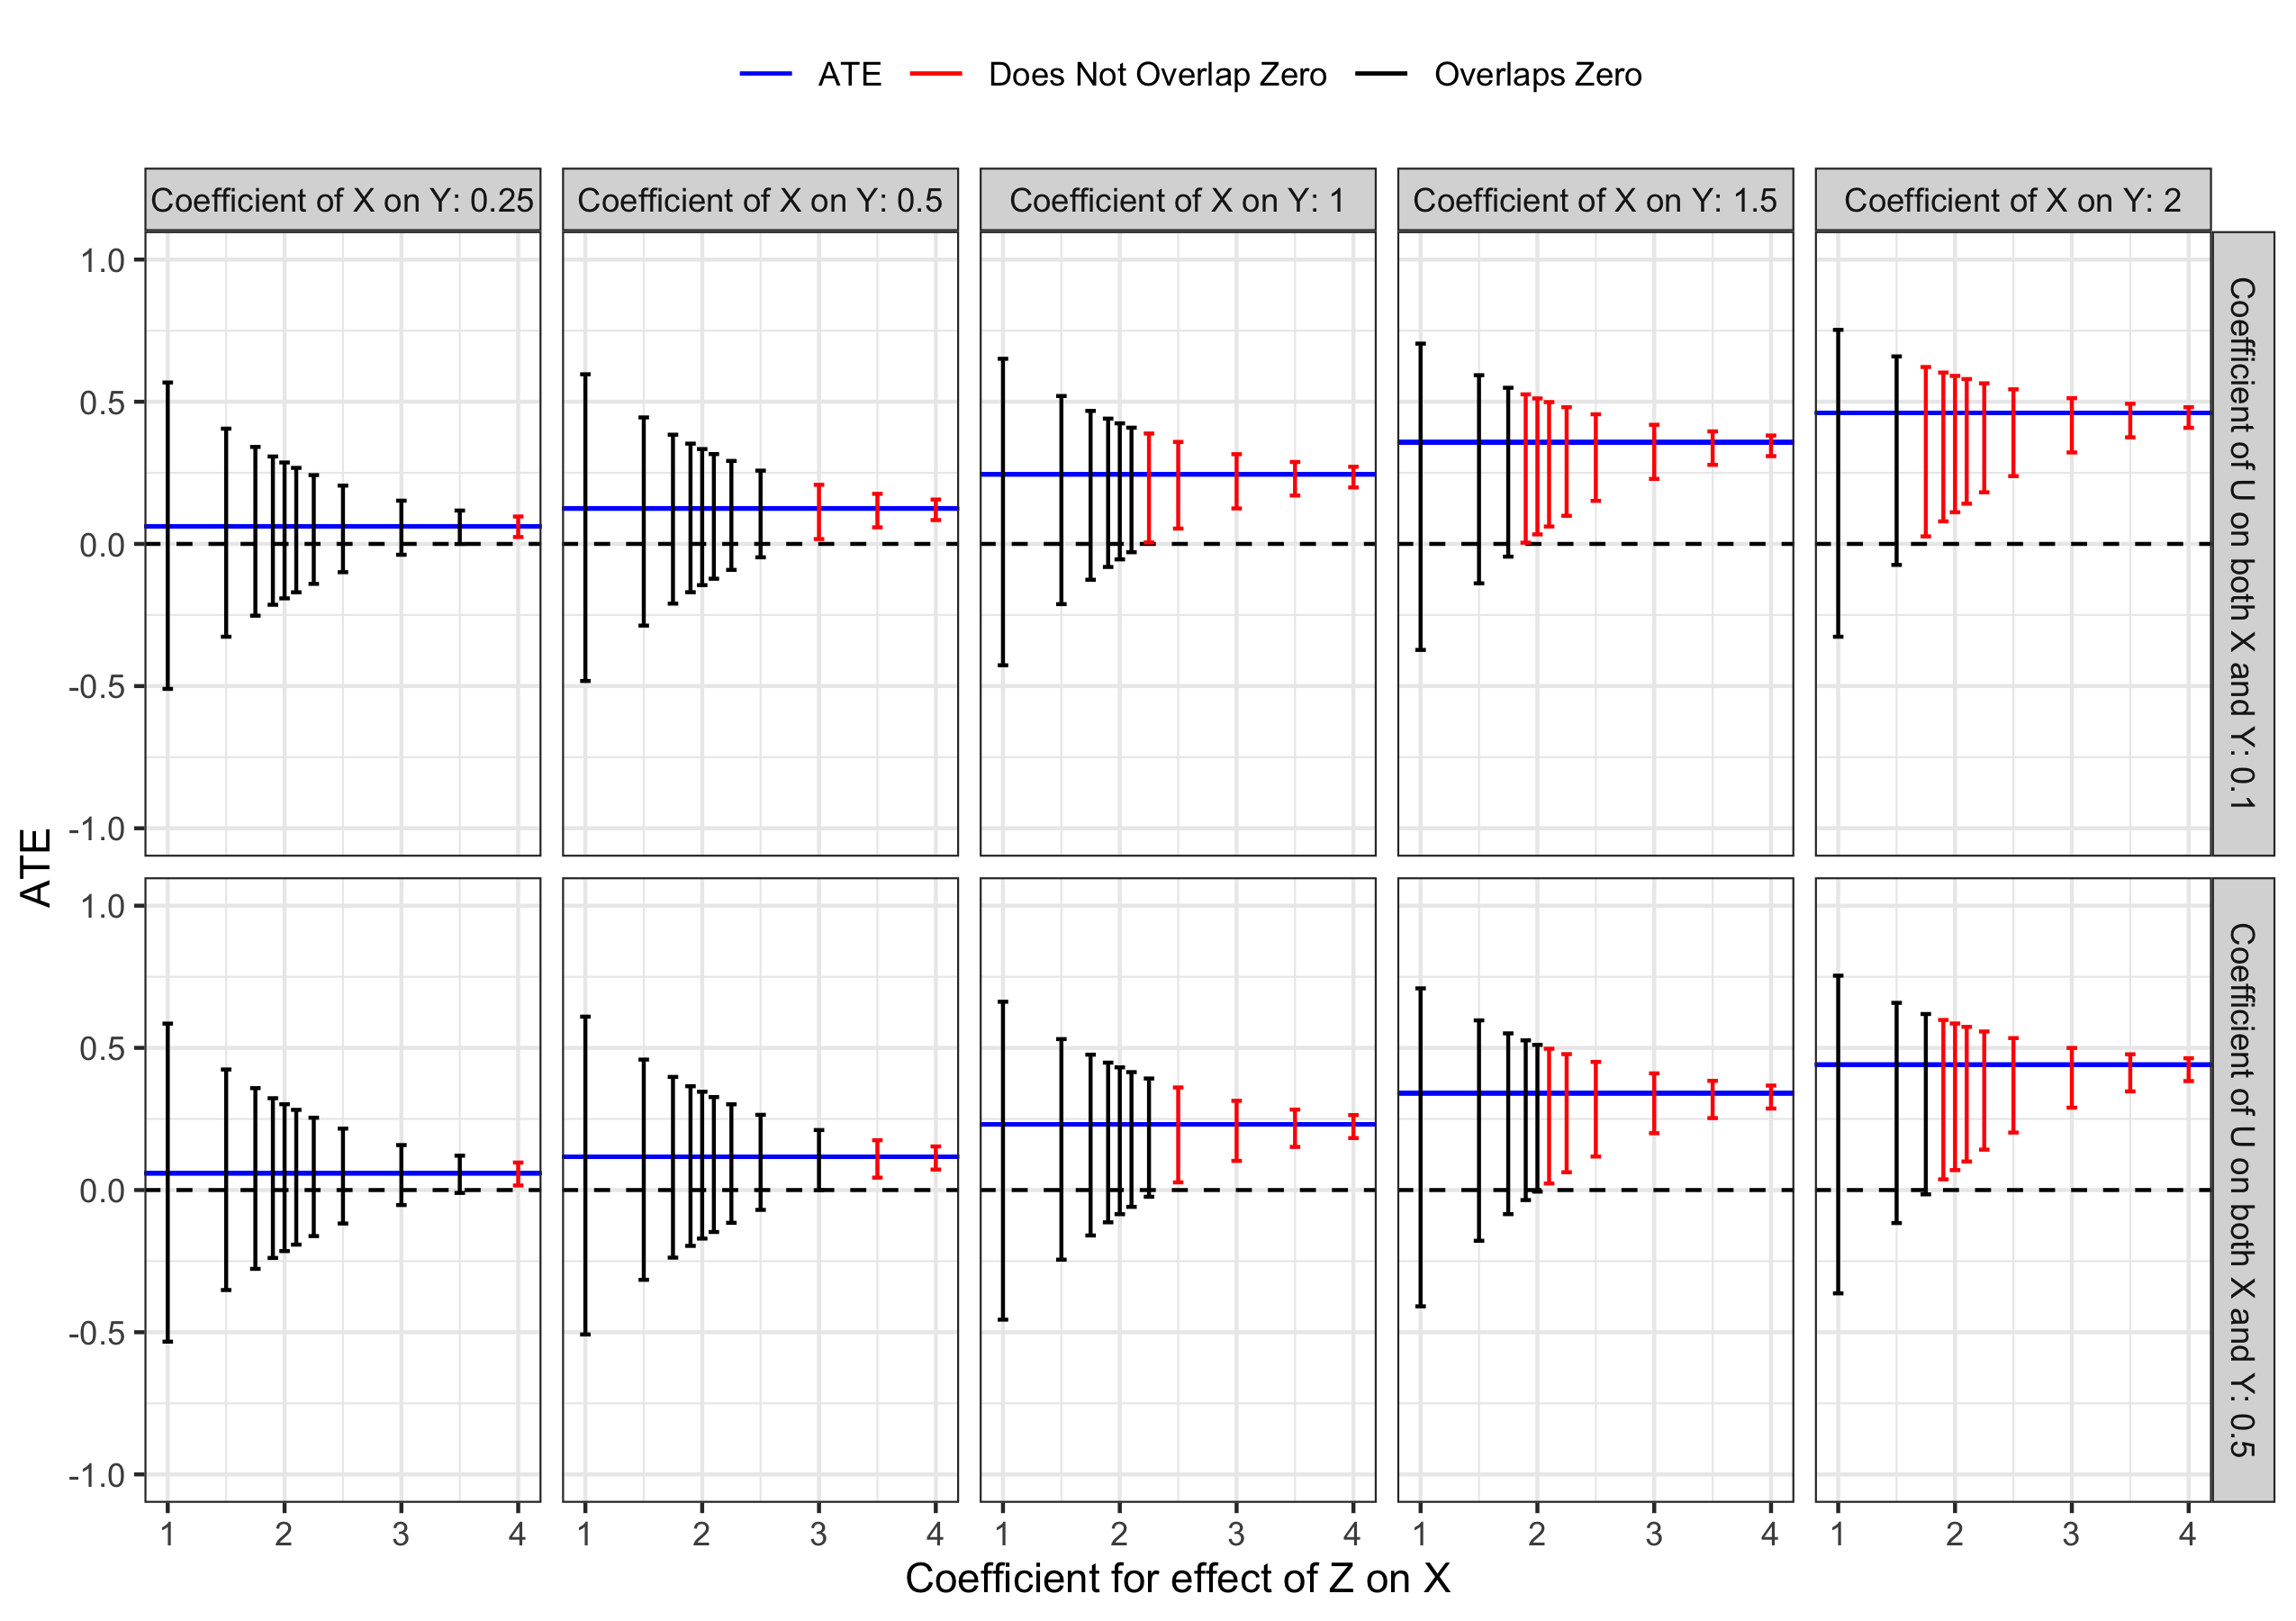
\includegraphics[width=0.99\textwidth]{/Users/ralphtrane/Documents/RPackages_dev/ACEBounds/figures/power.png}
  \caption{Bounds based on simulations as described in Section \ref{properties-of-bounds-from-summary-level-data}. Upper and lower bounds are connected a curve based on a loess extrapolation. This curve is used to find the smallest coefficients needed to detect direction as plotted on Figure \ref{fig:power_curves}.}
  \label{fig:power}
\end{figure}

To find the smallest value of \(\gamma_1\) that results in bounds excluding \(0\), we fit a loess curve to the lower bounds in Figure \ref{fig:power}, and find the value where this curve crosses \(0\). This results in the values depicted on Figure \ref{fig:power_curves}.

\hypertarget{bounds-from-two-sample-data-with-multiple-ivs}{%
\section{\texorpdfstring{Bounds From Two Sample Data With Multiple IVs \label{appendix-sim-results-multiple-IVs}}{Bounds From Two Sample Data With Multiple IVs }}\label{bounds-from-two-sample-data-with-multiple-ivs}}

Here, we will describe how to expand the monte carlo integration to include multiple IVs. Consider the exposure and outcome models introduced in Appendix \ref{appendix-logistic-models}. \(z_i \in \{0,1,2\}\) represents the \(i\)th instrument, and \(\gamma_i\) represents the \(i\)th instrument's effect on the exposure. Also, for each instrument \(i\), we set \(P(Z_i = 0) = P(Z_i = 2) = 0.25\) and \(P(Z_i = 1) = 0.5\). We set \(p = 10\) or \(p = 50\), and draw \(U\) from a standard normal distribution. Again, for simplicity, we set \(\beta_U = \gamma_U\), and \(\gamma_0 = -\sum_i \gamma_i\) and \(\beta_0 = -\beta_1/2\) to spread out the probabilities \(P(X = 1 | Z = z)\) and \(P(Y = 1 | X = x)\) as much as possible. \(\beta_1\) is set to be either \(0.25\), \(0.5\), \(1\), \(1.5\), or \(2\). We then consider four scenarios for setting the \(\gamma_i\)'s:

\begin{enumerate}
\item \emph{Many weak instruments}: \(\gamma_i\) are spread out evenly on the interval \(0\) to \(0.2\).
\item \emph{Many strong instruments}: \(\gamma_i\) are spread out evenly on the interval \(1\) to \(4\). This is the magnitude of $\gamma$s that detected the direction of the ATE in the previous section
\item \emph{Many very weak instruments, one medium strength instrument}: $\gamma_i$, $i=1,2,...,p-1$, are evenly spread out on the interval $0$ to $0.01$, and $\gamma_p = 0.2$. 
\item \emph{Many medium strong instruments, one strong instrument}: $\gamma_i$, $i=1,2,...,p-1$, are evenly spread out on the interval $1$ to $1.2$, and $\gamma_p = 4$.
\end{enumerate}

The first scenario mimics typical magnitudes of coefficients seen in MR studies, and is an example where many genetic traits weakly contribute to the expression of complex traits \autocite{loh_contrasting_2015,shi_contrasting_2016,nj_genetic_2017}. The third scenario represents a genetic architecture where only few genetic variants have strong effects on the exposure while others have weak effects \autocite{yang_common_2010}. Scenarios 2 and 4 are as scenarios 1 and 3, but with coefficients of larger magnitude. We don't expect to observe this in practice, but these are the magnitudes that our results in Section \ref{bounds-from-bivariate-data} suggests would result in informative bounds when \(p = 1\).

For each scenario, we use monte carlo integration with \(1,000,000\) re-samples to obtain \(P(X = 1 | Z_j = z_j)\) and \(P(Y = 1 | Z_j = z_j)\) -- this procedure is as described in Appendix \ref{appendix-sim-results}. We then use these quantities to obtain two-sample IV bounds for each of the \(p\) instruments. Figures \ref{fig:bounds_from_multiple_IV_sims_MR}, \ref{fig:bounds_from_multiple_IV_sims_MR_many_weak}, \ref{fig:bounds_from_multiple_IV_sims_power}, and \ref{fig:bounds_from_multiple_IV_sims_power_many_weak} summarize the results. We see that in scenarios 1 and 2, every bound is non-informative, with widths close to or exceeding \(1\). Also, the bounds are nested within each other. Thus, if we were to aggregate the bounds by taking intersections, the width of the intersection bounds will still be close to or exceed \(1\). In addition, the increase in magnitude of the \(\gamma_i\) coefficient did not improve the bounds. Scenarios 3 and 4 show similar results in that the bounds cover the null effect, but the strongest instrument in each scenario produces a much smaller bound than in scenarios 1 and 2. From Figure \ref{fig:multiple_IVs_scenario_3} it is clear that on the scale that is often observed in MR studies, two-sample nonparametric bounds are generally non-informative. Also, the bounds in scenarios 3 and 4 are again nested leaving us with the conclusion that the intersection of bounds from multiple instruments will give no more information than the strongest of the instruments itself.

We take a moment to explain the differences between our result in Section \ref{bounds-from-bivariate-data} with a single instrument with \(\gamma_i = 4\) and our results in this section where one of the instruments has \(\gamma_i = 4\), but others have much smaller \(\gamma\)s. We see that if the variation in the exposure model is determined by multiple independent instruments, the effect of one single instrument on producing an informative bound greatly diminishes. Specifically, Figure \ref{fig:multiple_IVs_scenario_4} shows that in a setting where we would be able to detect the direction of the ATE from an instrument with \(\gamma_i = 4\) if only \(p = 10\) instruments are contributing to the exposure, that same coefficient would not be large enough if \(p = 50\) instruments were included. This suggests that for exposures that are determined by many instruments, the strongest among these instruments must be even stronger for a bound-based analysis to be useful. In other words, multiple instruments may not be helpful in a bound-based analysis when the exposure is polygenic in nature.

Our results also have dire implications when some instruments turn out to be invalid. If, as suggested by \textcite{swanson_commentary_2017}, we take the union of IV bounds so that the union bound is guaranteed to cover the true ATE so long as there is at least one valid instrument, the union bound will likely be non-informative because there was at least one IV bound in our scenario that was non-informative. Without making some assumptions about the nature of the invalid IVs, it would generally be infeasible to obtain useful information from a bound-based analysis.

Overall, combining our results in Section \ref{bounds-from-bivariate-data}, our conclusion about using nonparametric IV bounds in two-sample MR studies is grim. Such a nonparametric analysis would require very strong instruments and/or effect sizes, which are rare in MR studies, and even stronger than those in one-sample settings. Also, multiple instruments are no better than having a single, strong instrument. As discussed in Section \ref{bounds-from-bivariate-data}, a primary reason for the non-informative nature of the IV bounds in two-sample settings is that we don't have information about the joint distribution of \(X,Y\) given \(Z\). While obtaining this joint distribution is generally difficult in many MR studies, in the next section, we discuss how to obtain a plausible range of the joint distribution \(P(Y, X | Z)\) given two sample MR data \(P(Y|Z)\) and \(P(X | Z)\) in order to create more informative bounds from two-sample MR studies.

\begin{figure*}
  \centering
  \begin{subfigure}{0.5\linewidth}
  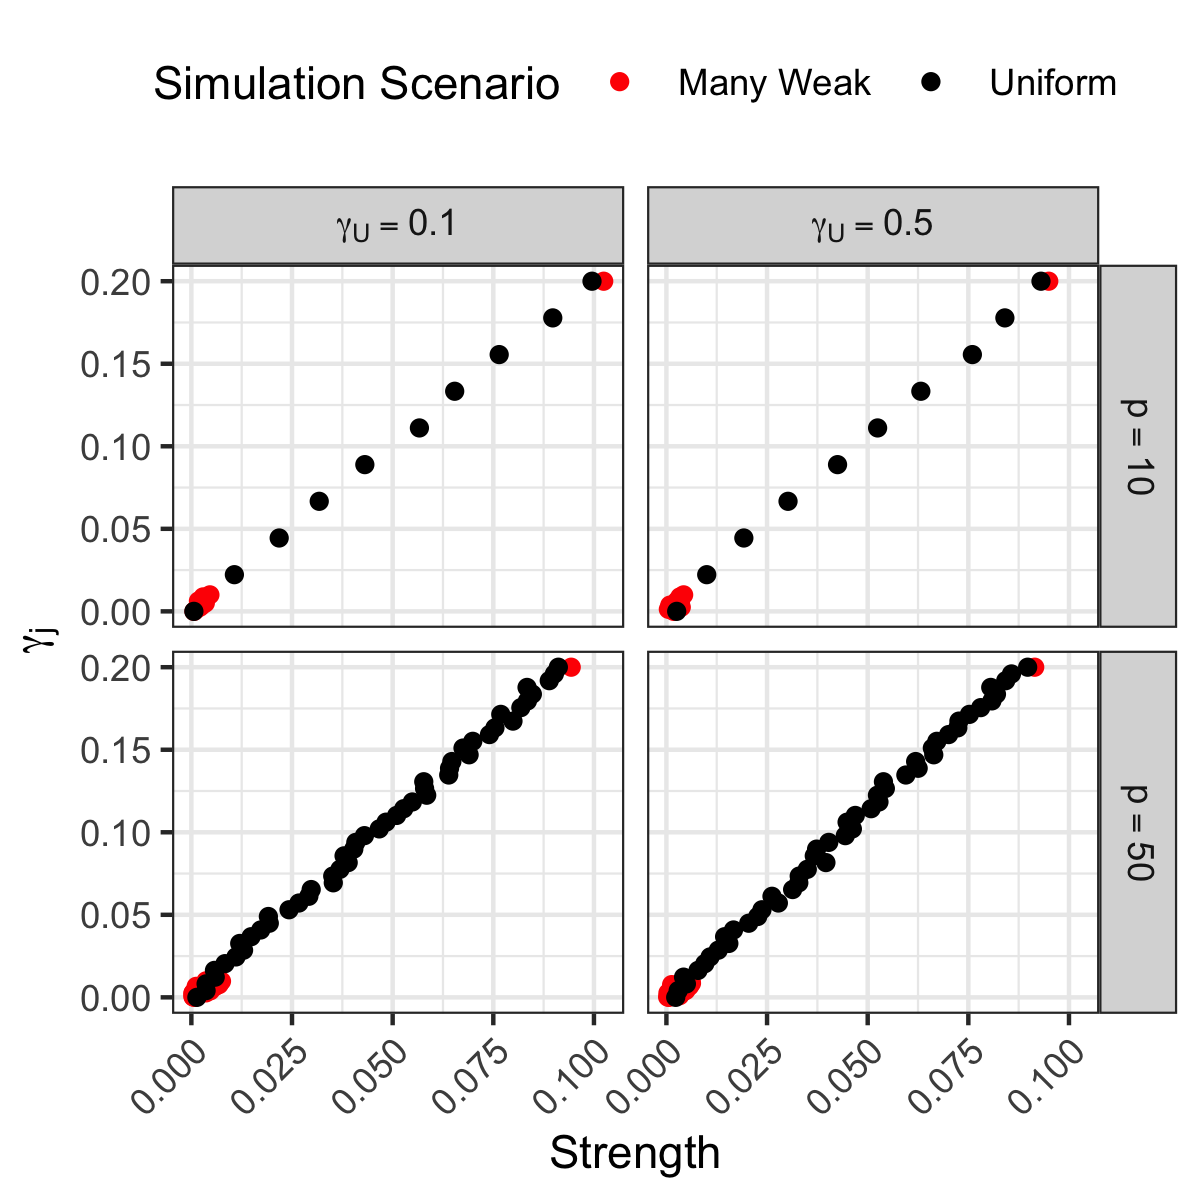
\includegraphics[width=\textwidth]{/Users/ralphtrane/Documents/RPackages_dev/ACEBounds/figures/strength_vs_coef_multiple_IVs_MR.png}
  \caption{Scenarios 1 and 3}
  \label{fig:strength_vs_coef_multiple_IVs_MR}
  \end{subfigure}%
  ~
  \begin{subfigure}{0.5\linewidth}
  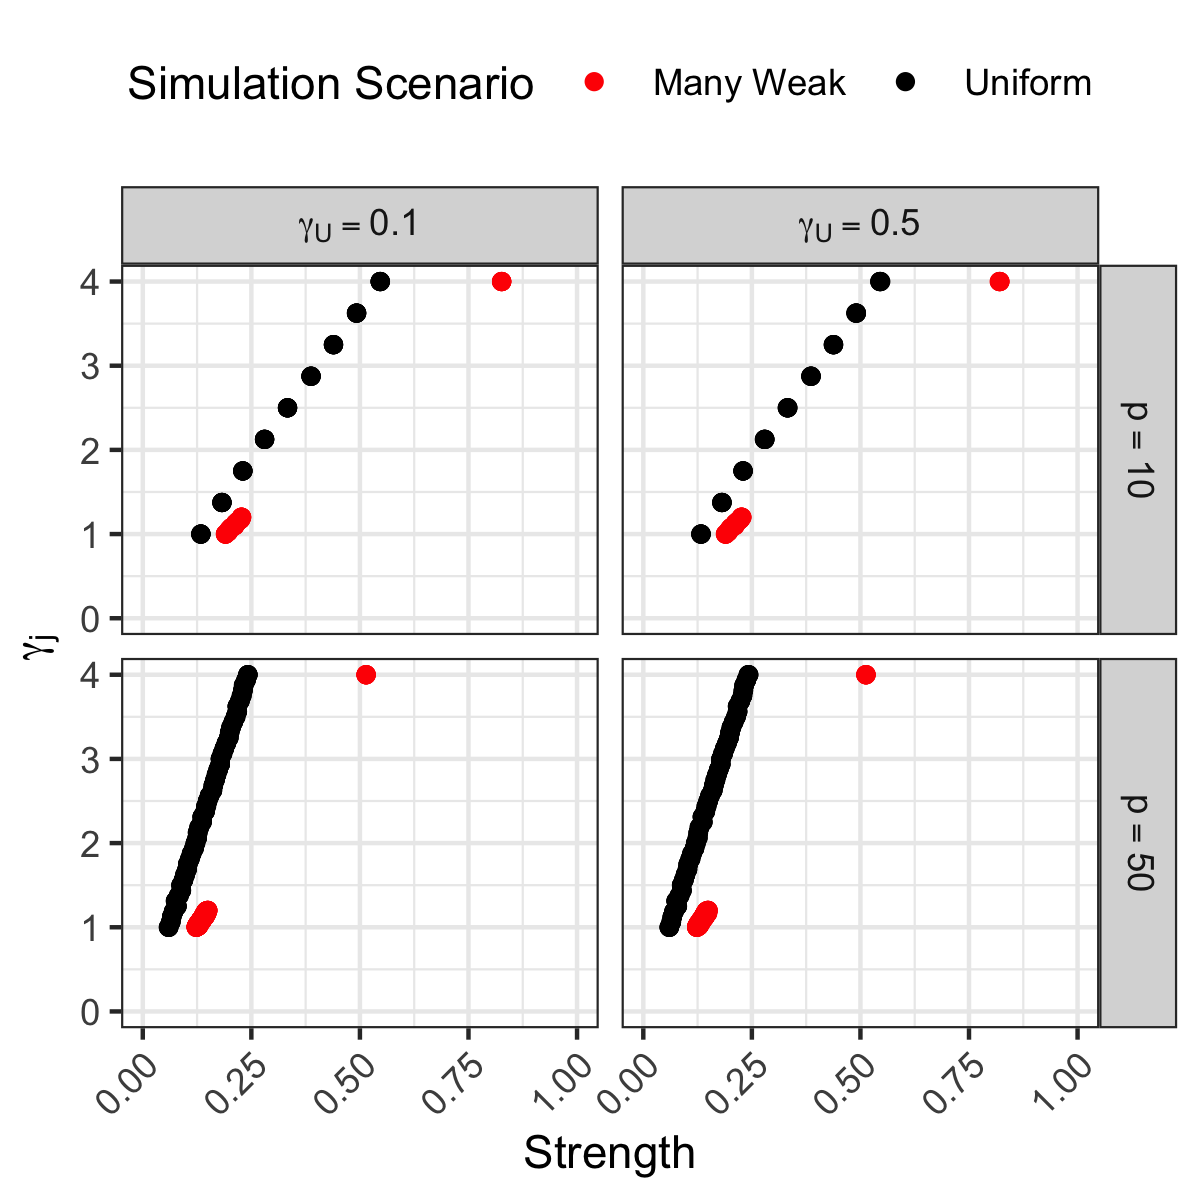
\includegraphics[width=\textwidth]{/Users/ralphtrane/Documents/RPackages_dev/ACEBounds/figures/strength_vs_coef_multiple_IVs_power.png}
  \caption{Scenarios 2 and 4}
  \label{fig:strength_vs_coef_multiple_IVs_power}
  \end{subfigure}
  \caption{Figure showing the dilution effect described in Section \ref{bounds-from-two-sample-data-with-multiple-ivs} in each of the four scenarios. When $p$ is larger, similar sized coefficients lead to lower strength. The effect is smaller when we are in a scenario where one coefficient is relatively much larger than the rest, rather than when the coefficients are evenly spread out.}
  \label{fig:strength_vs_coef_multiple_IVs}
\end{figure*}

\clearpage

\begin{sidewaysfigure}
  \centering
  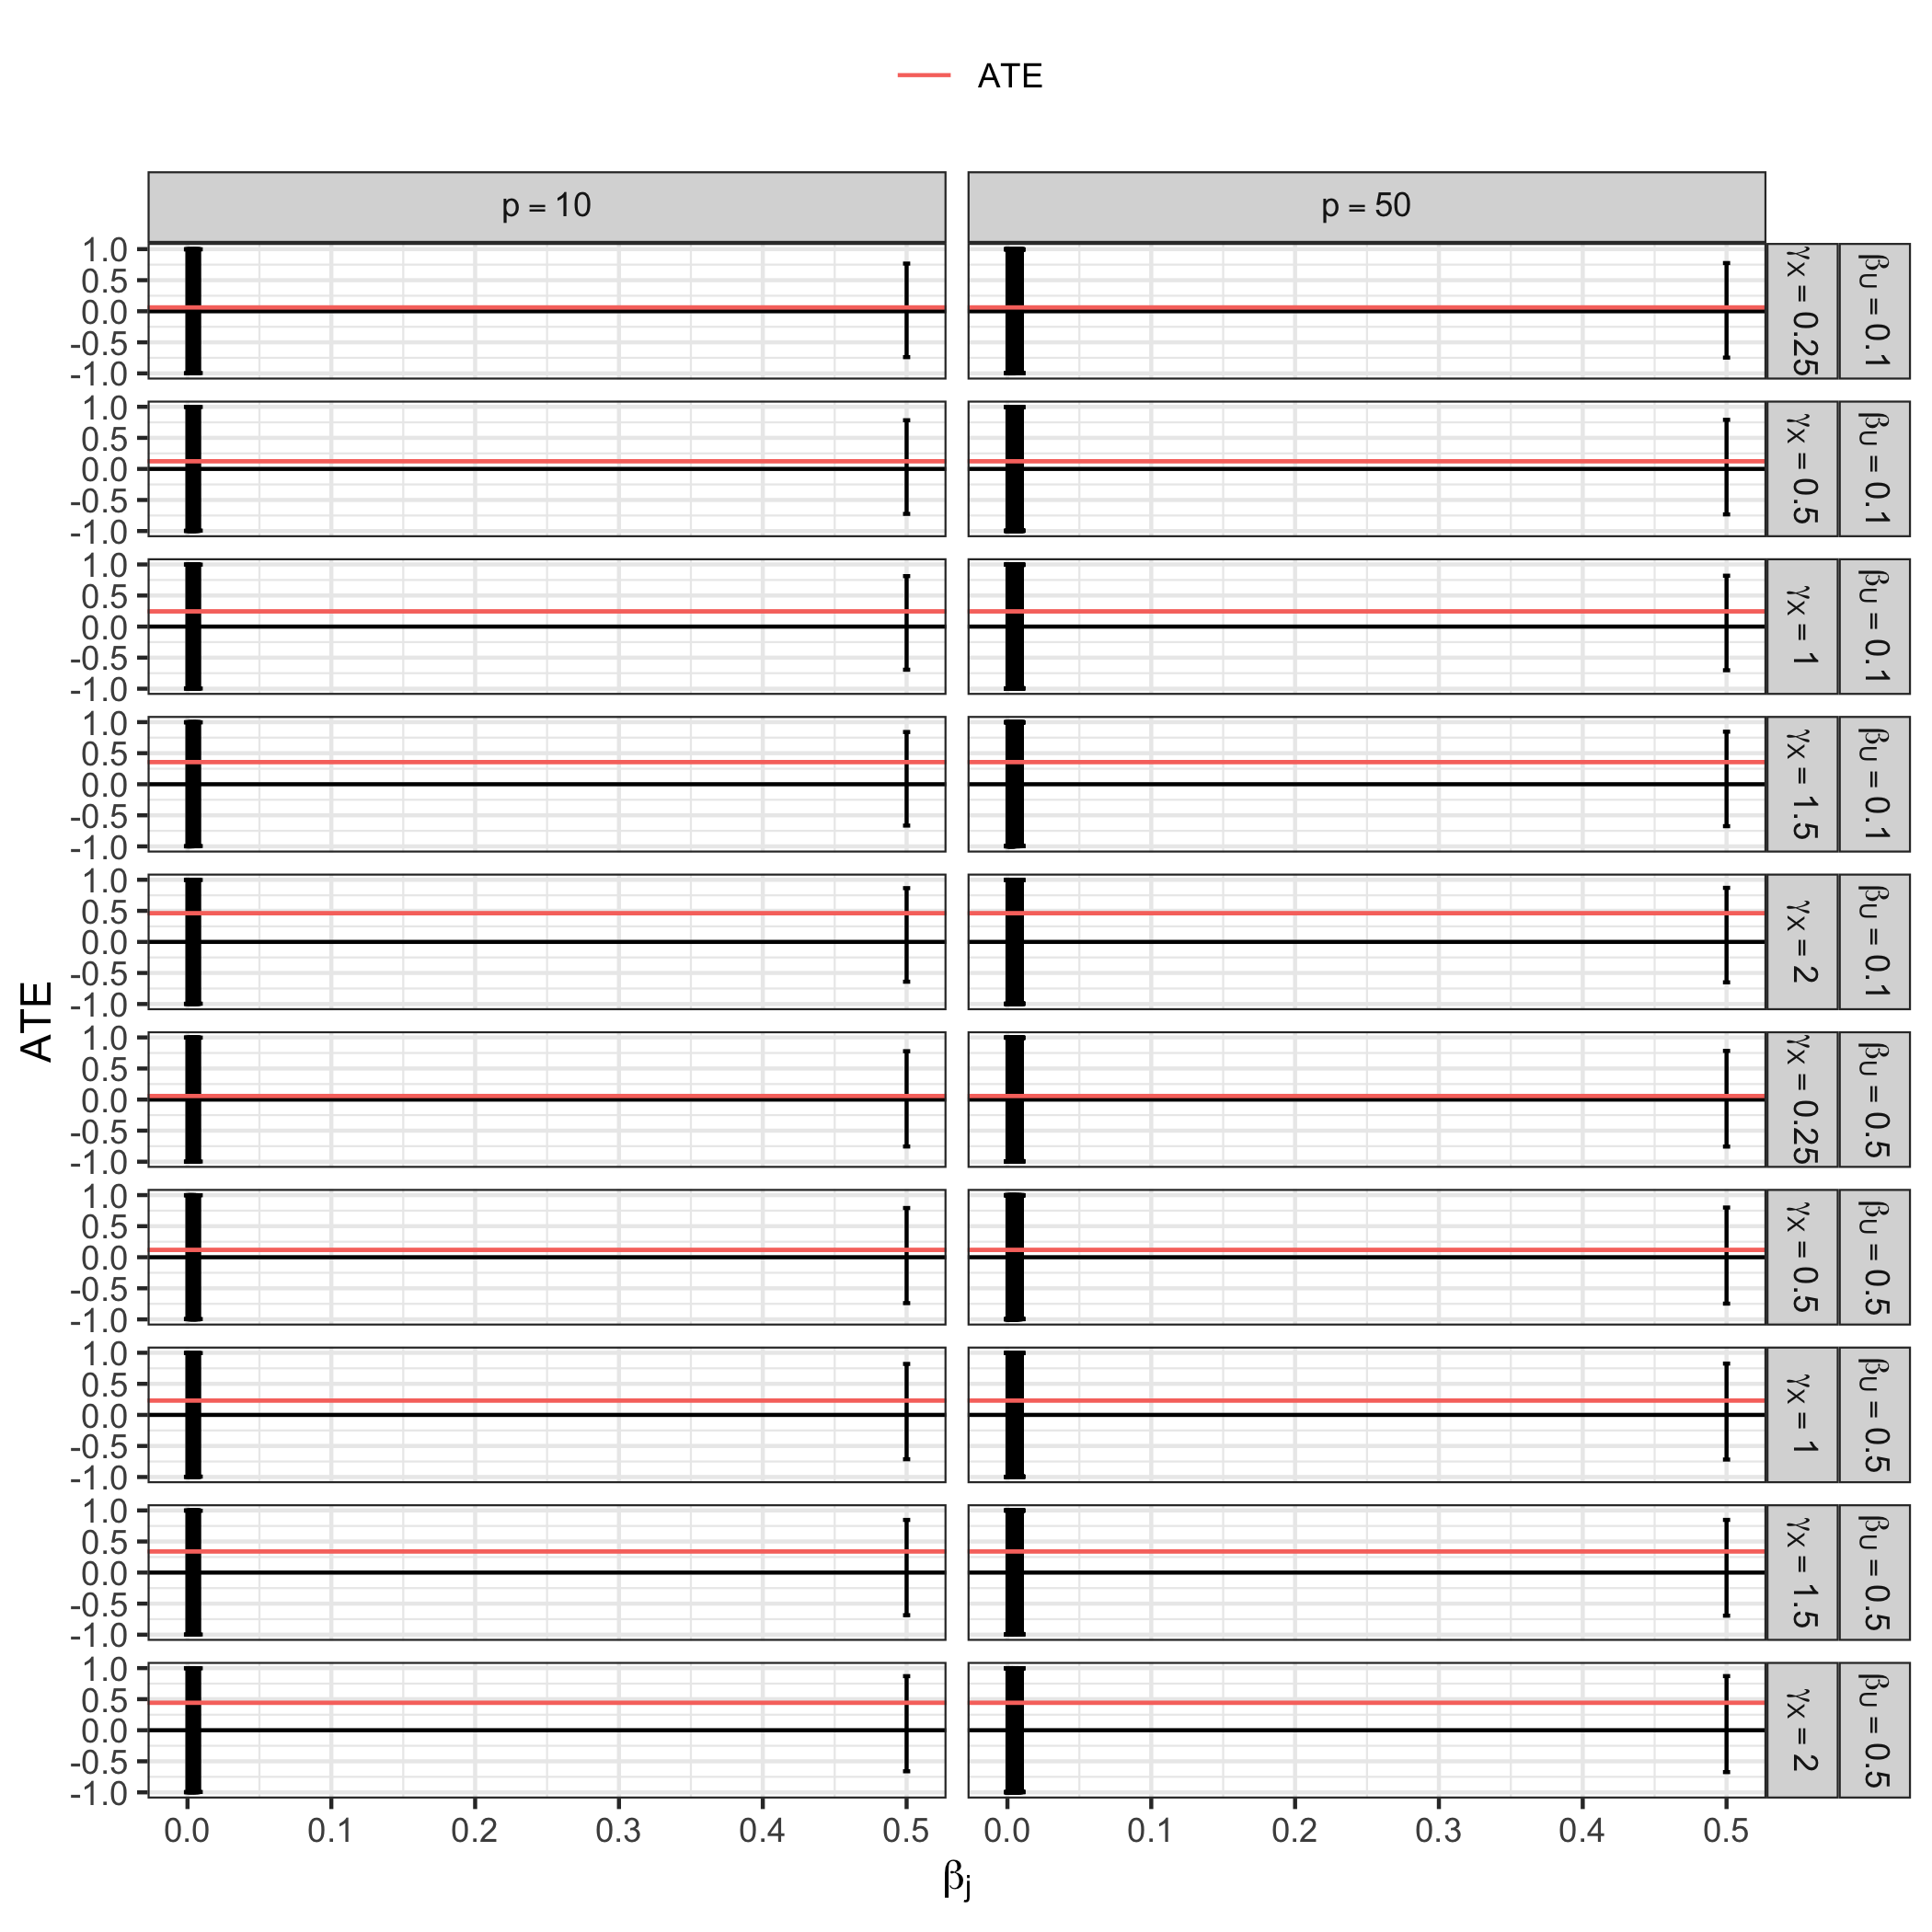
\includegraphics[width=\textheight]{/Users/ralphtrane/Documents/RPackages_dev/ACEBounds/figures/bounds_from_multiple_IV_sims_MR.png}
  \caption{Bounds based on monte carlo integration with 1,000,000 resamples in scenario 1.}
  \label{fig:bounds_from_multiple_IV_sims_MR}
\end{sidewaysfigure}

\clearpage

\begin{sidewaysfigure}
  \centering
  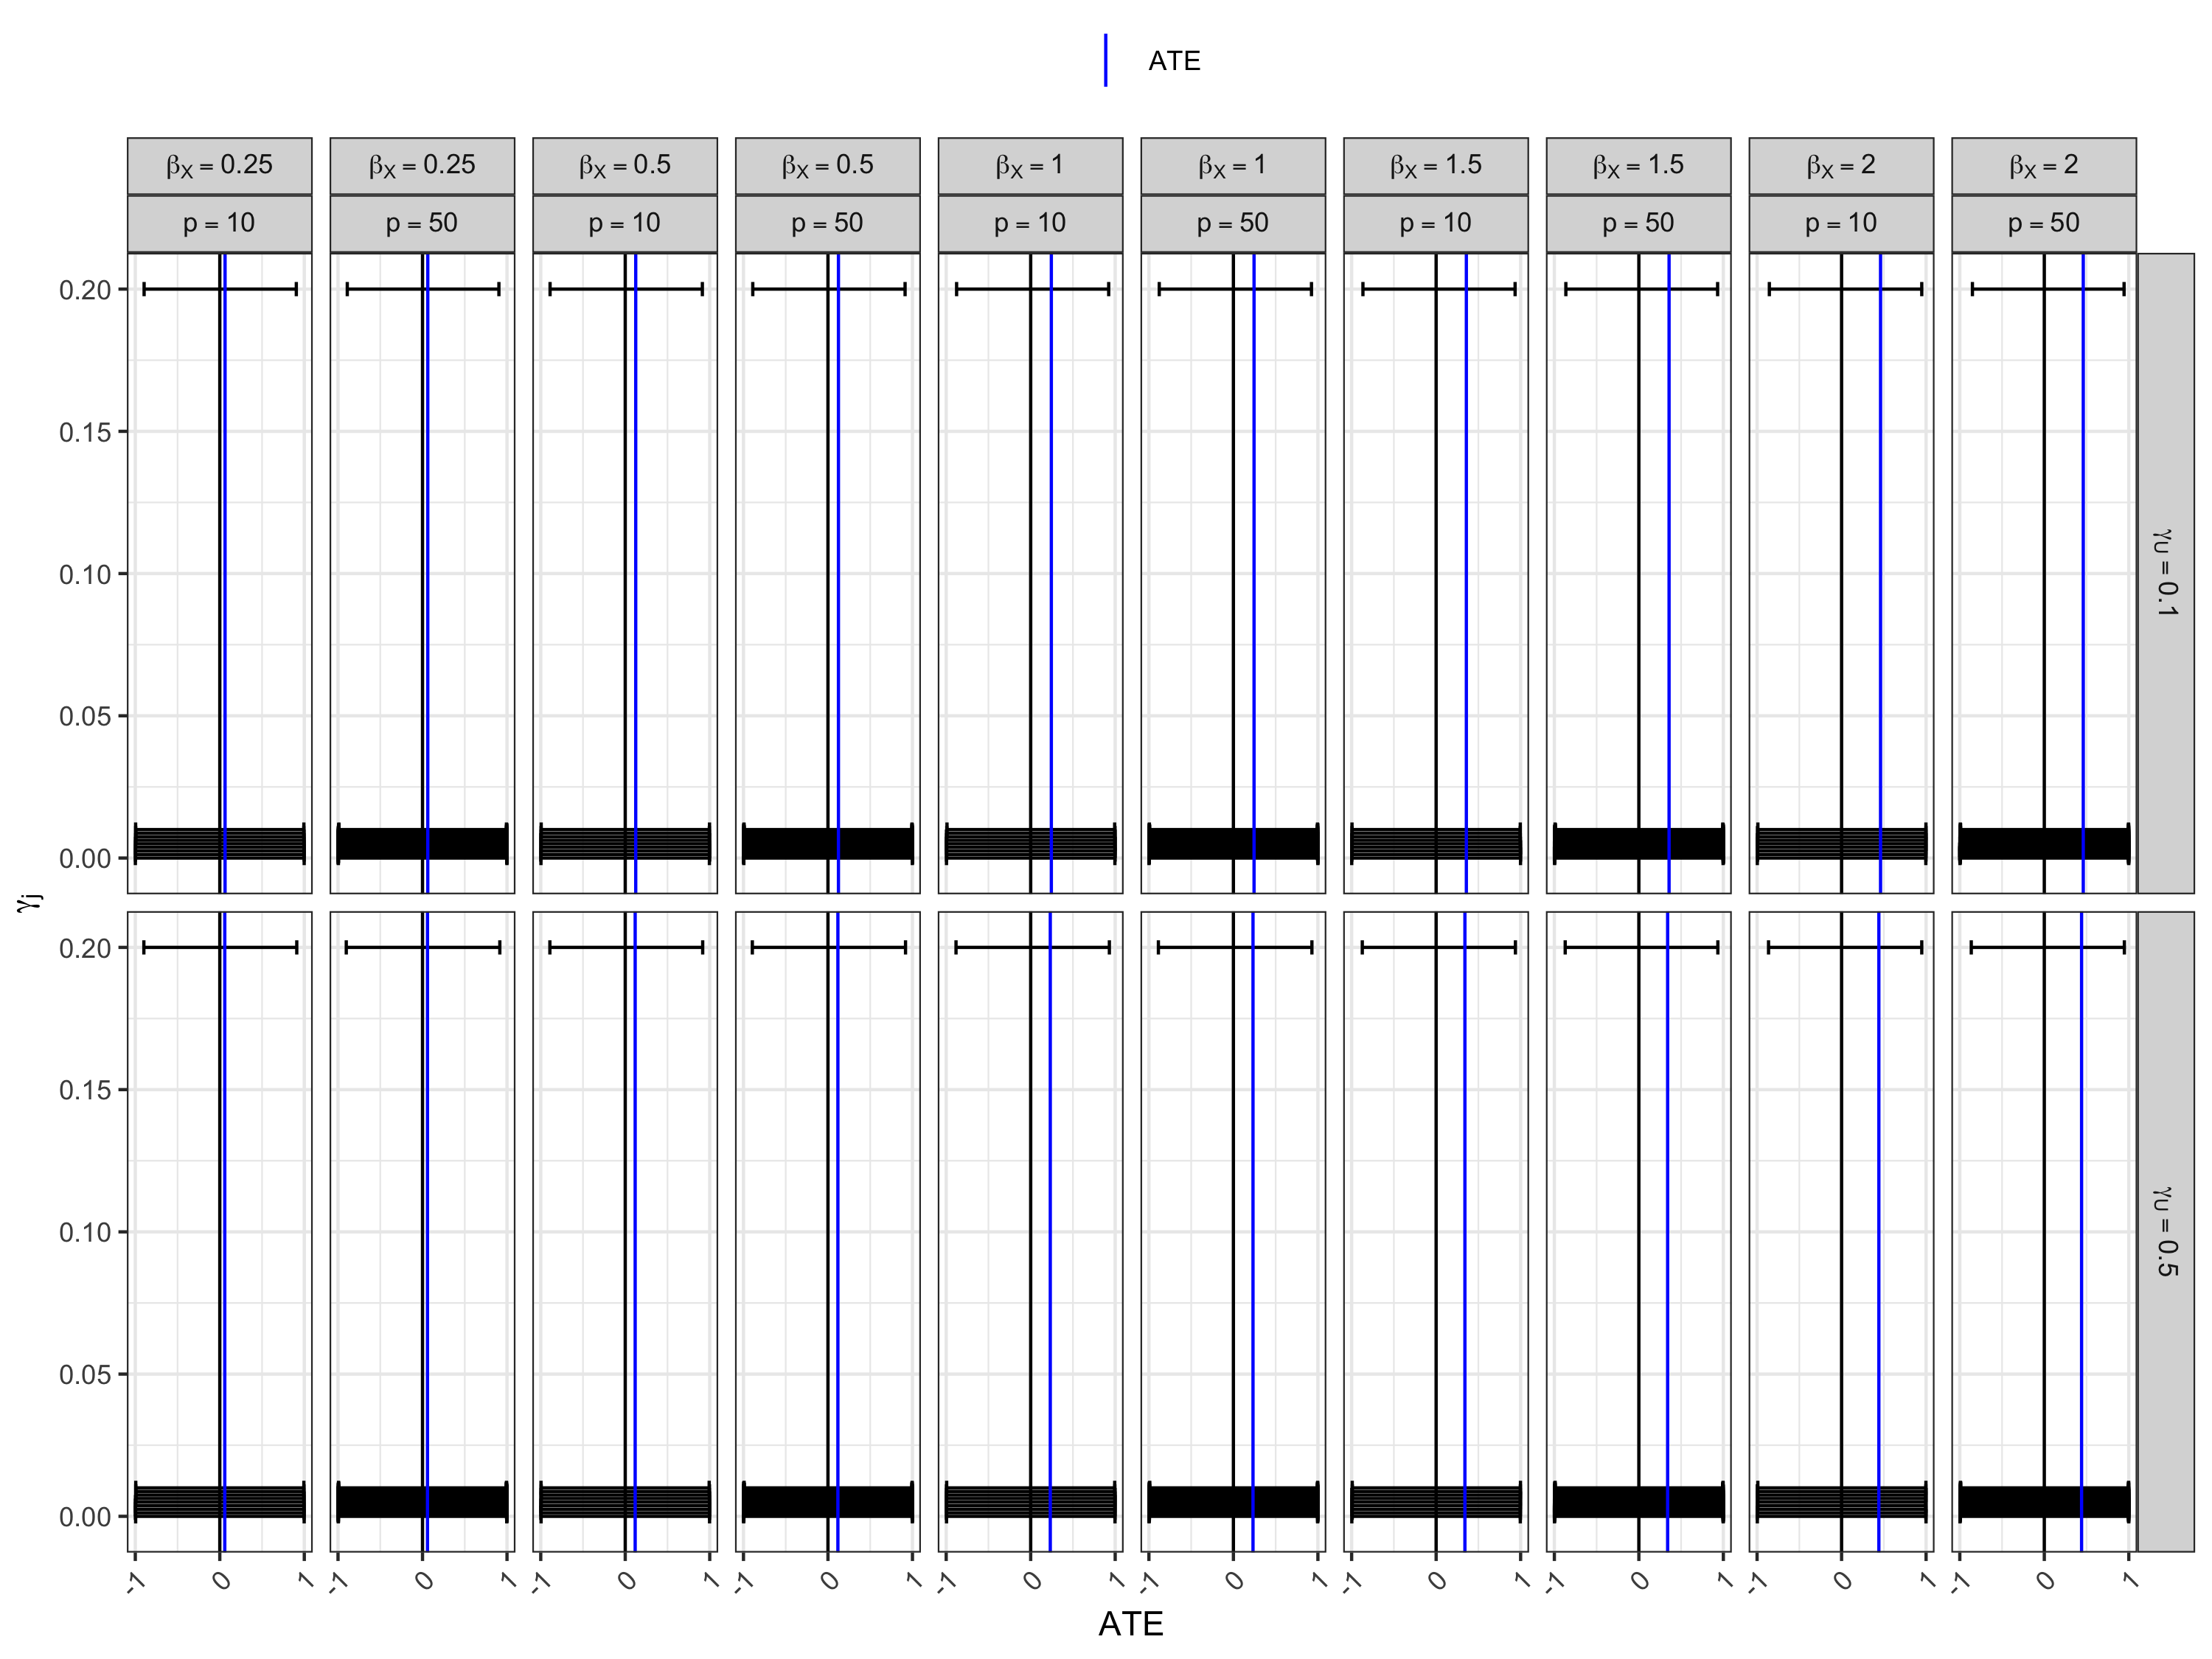
\includegraphics[width=\textheight]{/Users/ralphtrane/Documents/RPackages_dev/ACEBounds/figures/bounds_from_multiple_IV_sims_MR_many_weak.png}
  \caption{Bounds based on monte carlo integration with 1,000,000 resamples in scenario 3.}
  \label{fig:bounds_from_multiple_IV_sims_MR_many_weak}
\end{sidewaysfigure}

\clearpage

\begin{sidewaysfigure}
  \centering
  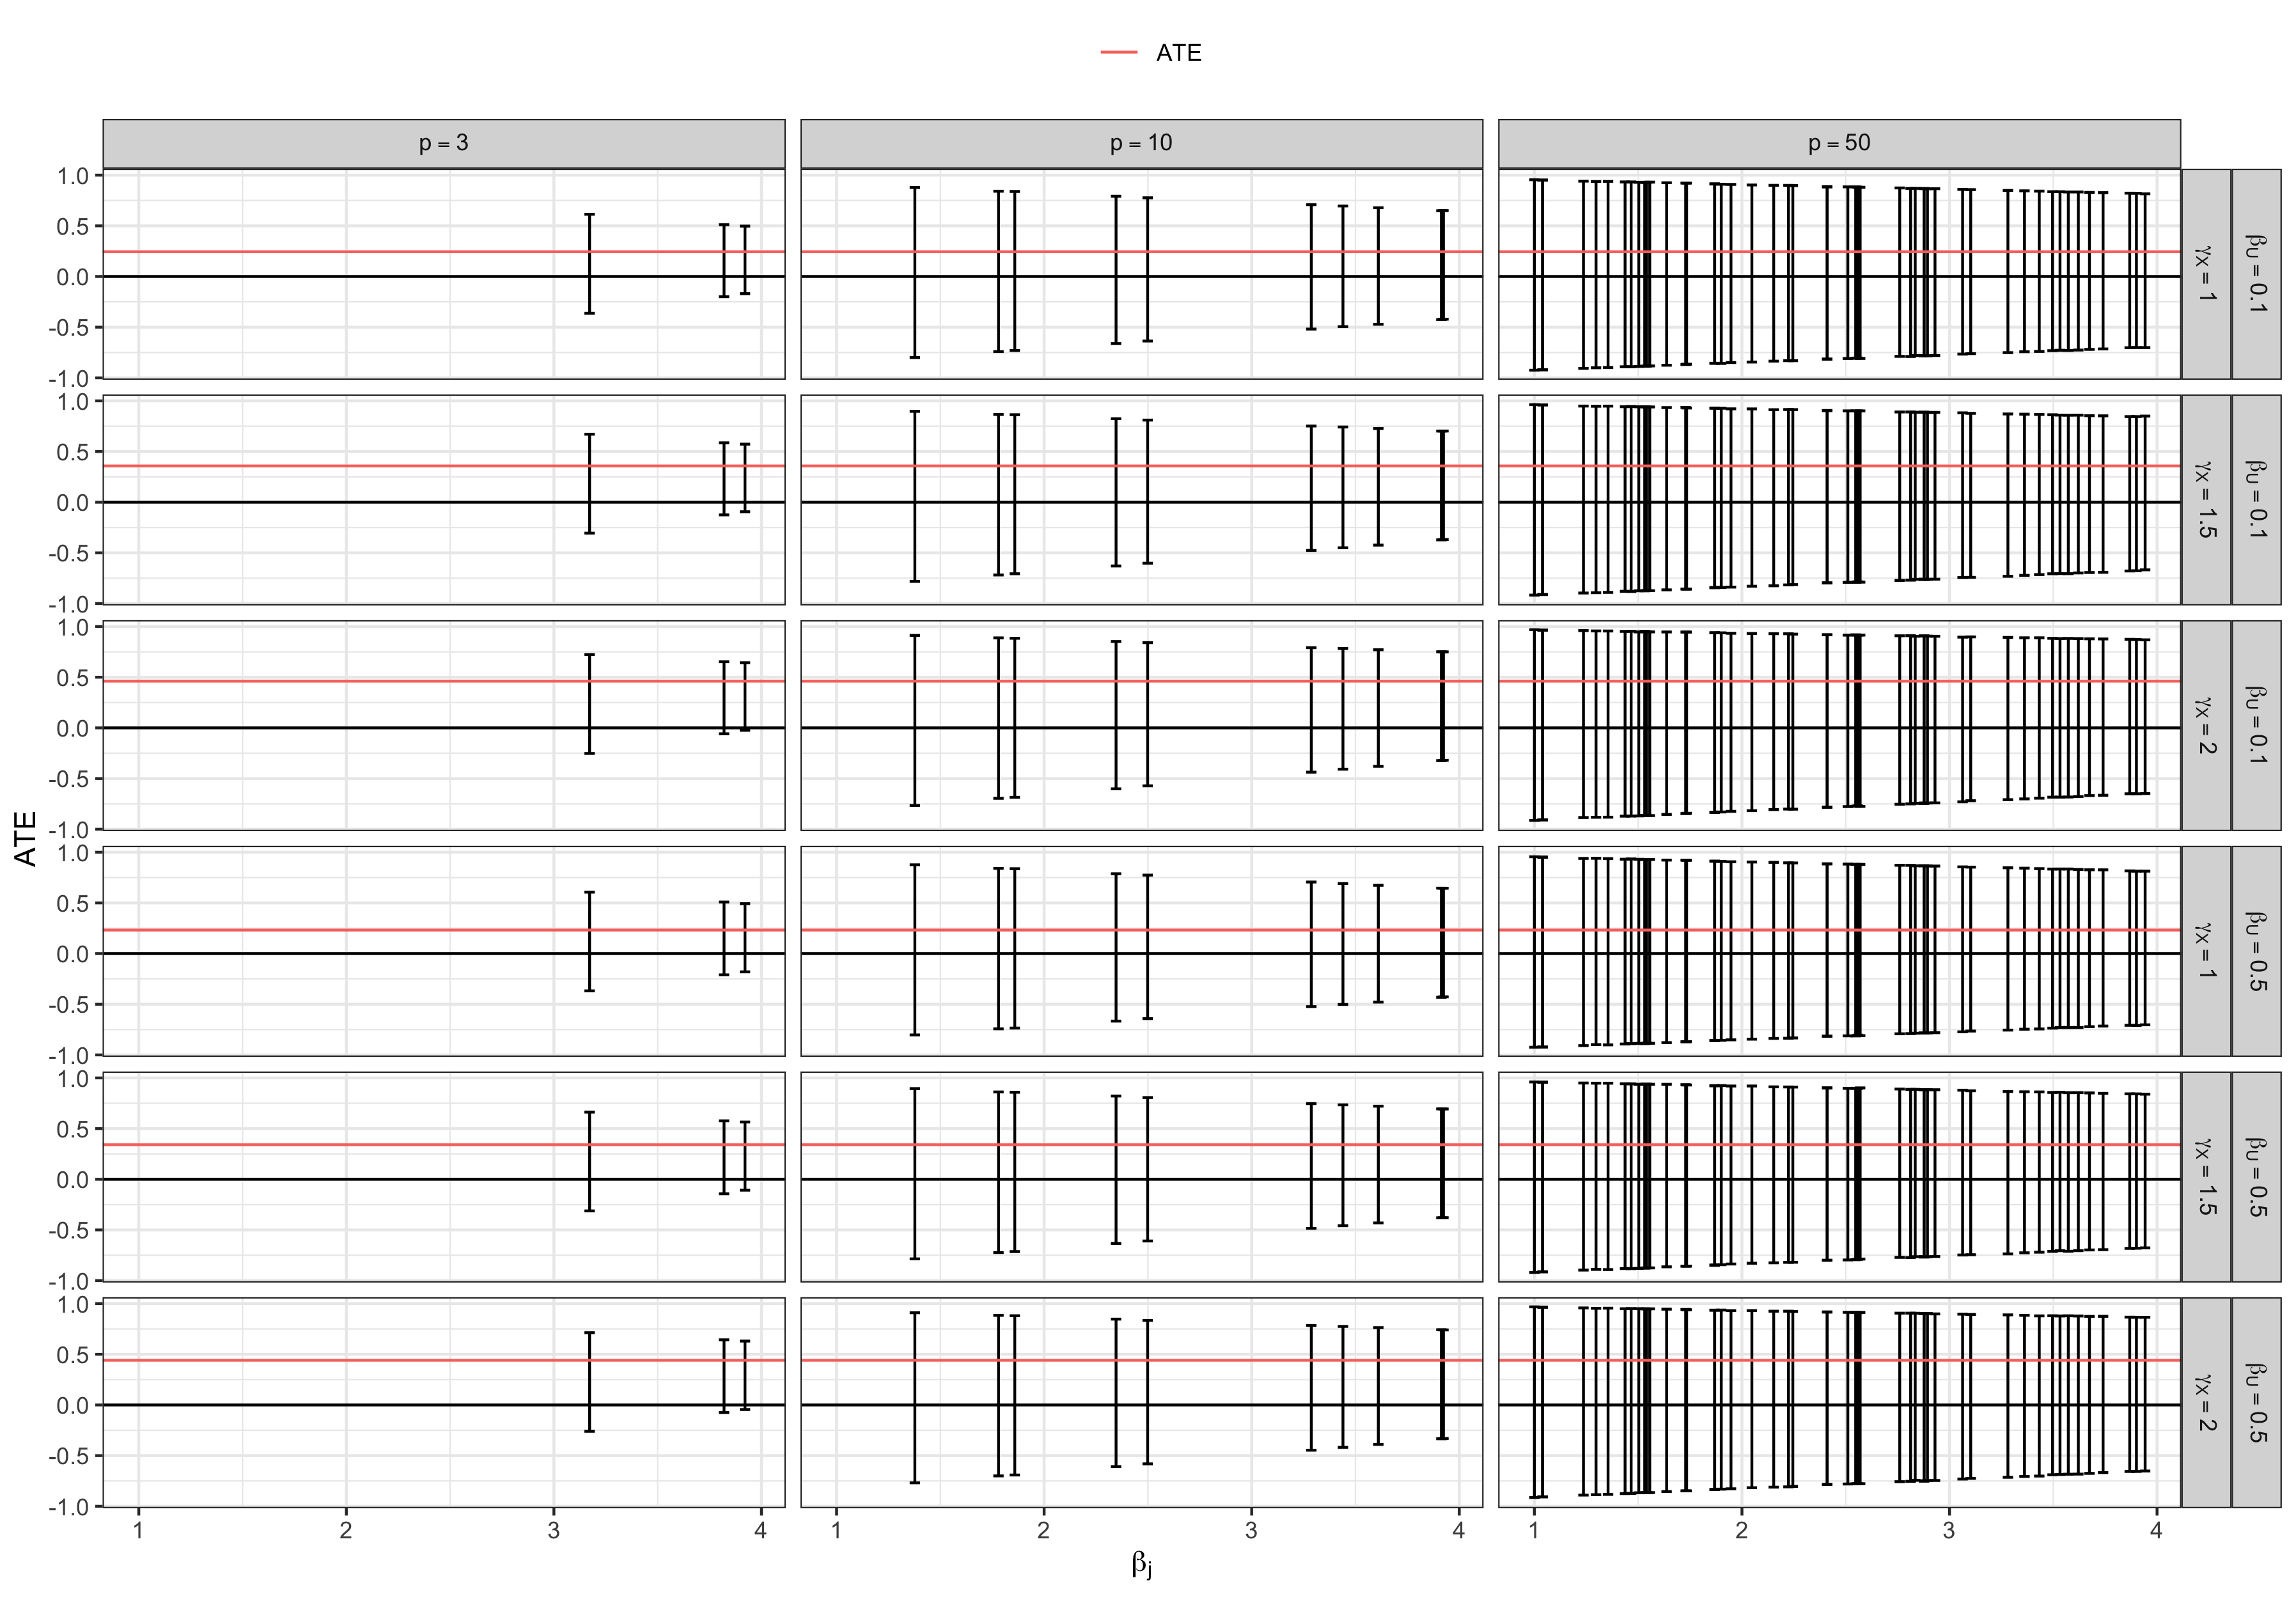
\includegraphics[width=\textheight]{/Users/ralphtrane/Documents/RPackages_dev/ACEBounds/figures/bounds_from_multiple_IV_sims_power.png}
  \caption{Bounds based on monte carlo integration with 1,000,000 resamples in scenario 2.}
  \label{fig:bounds_from_multiple_IV_sims_power}
\end{sidewaysfigure}

\clearpage

\begin{sidewaysfigure}
  \centering
  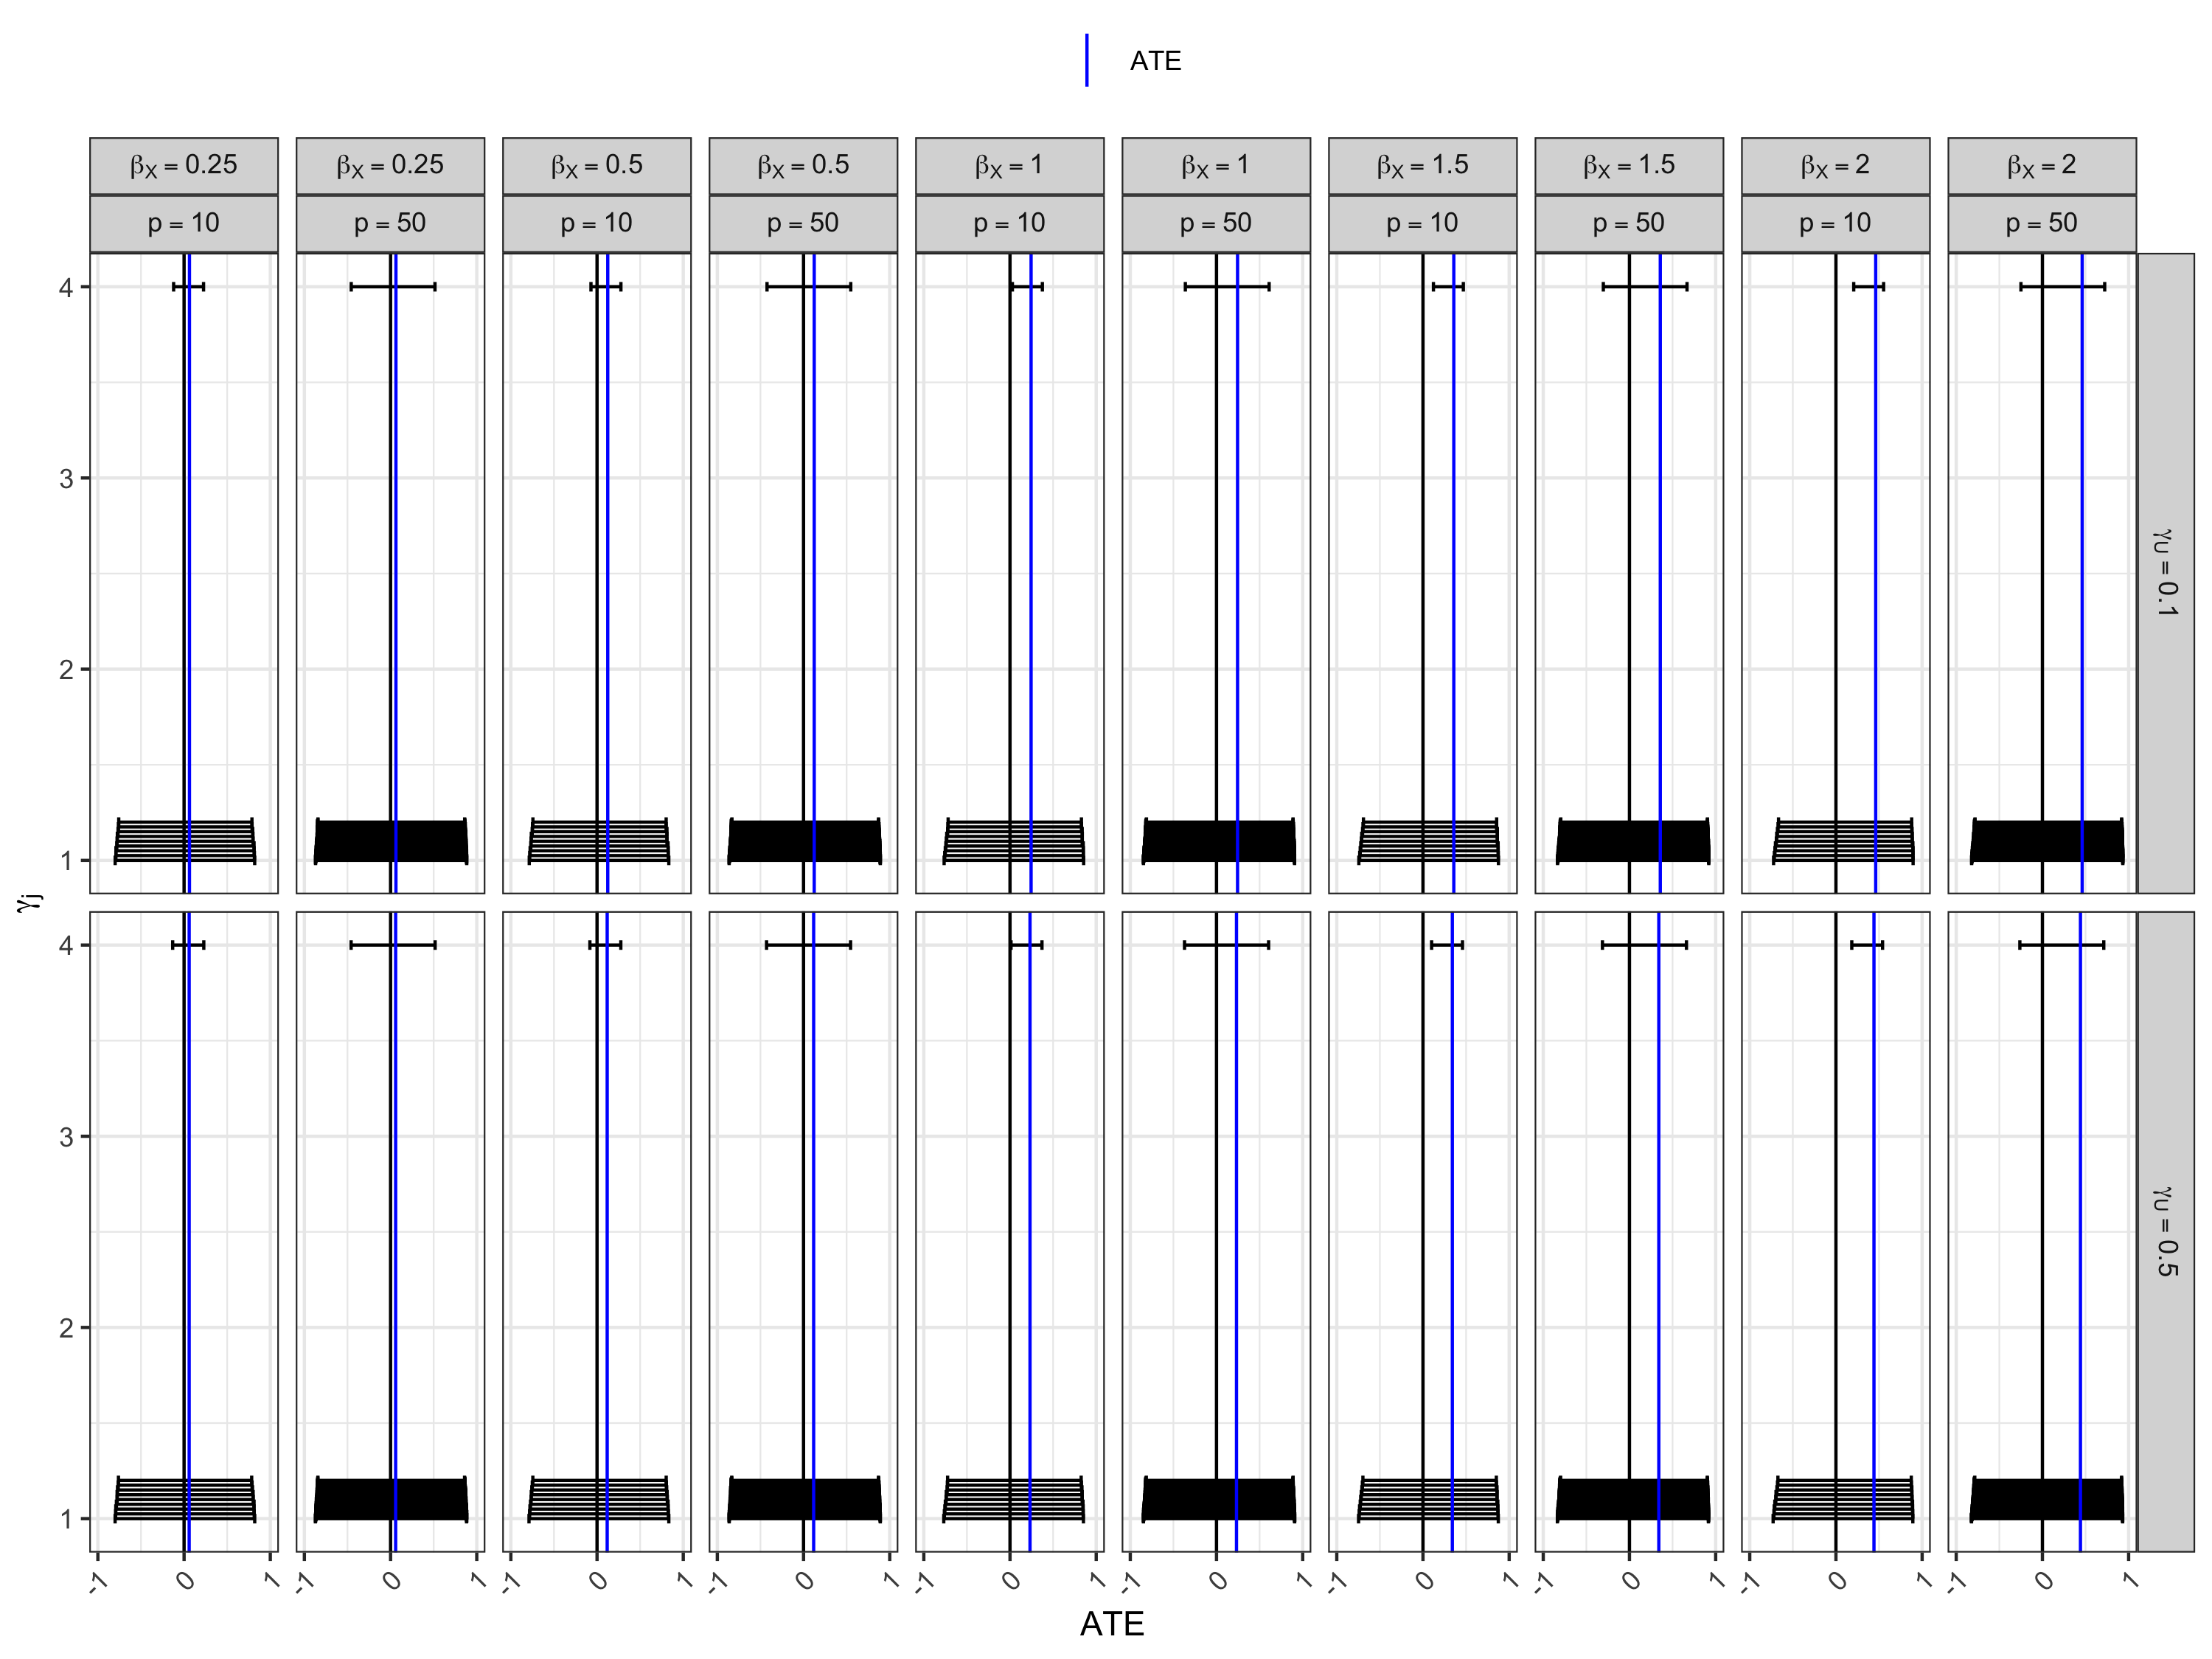
\includegraphics[width=\textheight]{/Users/ralphtrane/Documents/RPackages_dev/ACEBounds/figures/bounds_from_multiple_IV_sims_power_many_weak.png}
  \caption{Bounds based on monte carlo integration with 1,000,000 resamples in scenario 4.}
  \label{fig:bounds_from_multiple_IV_sims_power_many_weak}
\end{sidewaysfigure}

\clearpage

\hypertarget{reconstructing-the-joint-distribution-px-y-z}{%
\section{\texorpdfstring{Reconstructing the Joint Distribution \(P(X, Y | Z)\) \label{appendix-quasi-bayesian-details}}{Reconstructing the Joint Distribution P(X, Y \textbar{} Z) }}\label{reconstructing-the-joint-distribution-px-y-z}}

To draw a possible set of values for the joint conditional distribution \(P(X = x, Y = y | Z = z)\), we start by writing the joint conditional distribution \(P(X = x, Y = y | Z = z)\) as a function of the marginal conditional distributions \(P(X = x | Z = z)\) and \(P(Y = y | Z = z)\) and the conditional covariance of the exposure \(X\) and \(Y\) given \(Z=z\), \(\text{Cov}(X, Y | Z = z)\), for each \(z\)

\begin{equation}
P(X = x, Y = y | Z = z) = P(X = x | Z = z)P(Y = y | Z = z) + (2\cdot I[x = y] - 1)\text{Cov}(X, Y | Z = z). \label{eq:cov-expression}
\end{equation}

Because \(\text{Cov}(X, Y | Z = z)\) is impossible to estimate from two-sample MR studies, we instead propose to put a prior on this quantity. This prior must not only produce a proper probability distribution of \((X,Y|Z)\), but also satisfy the verifiable constraints \eqref{eq:constraints} from the IV assumptions. Specifically, by the definition of a proper probability distribution, \(\text{Cov}(X, Y | Z = z)\) must satisfy

\[
\begin{aligned}
  \max_z\left\{
      \begin{array}{c}
        -P(X = 1 | Z = z)P(Y = 1 | Z = z) \\
        -P(X = 0 | Z = z)P(Y = 0 | Z = z) \\
        P(X = 1 | Z = z)P(Y = 0 | Z = z) - 1\\
        P(X = 0 | Z = z)P(Y = 1 | Z = z) - 1
      \end{array}
    \right\} & \\
    \le \text{Cov}(X, &Y | Z = z) \le \\
    &\min_z\left\{
      \begin{array}{c}
        1 - P(X = 1 | Z = z)P(Y = 1 | Z = z) \\
        1 - P(X = 0 | Z = z)P(Y = 0 | Z = z) \\
        P(X = 1 | Z = z)P(Y = 0 | Z = z) \\
        P(X = 0 | Z = z)P(Y = 1 | Z = z)
      \end{array}
    \right\}
\end{aligned}
\]

Additionally, by the IV inequality constraints \(\max_x \sum_y \max_z P(X = x, Y = y | Z = z)\), for any pair of \((z_1, z_2) \in \{0,1,2\} \times \{0,1,2\}\), the values of \(\text{Cov}(X, Y | Z = z_1)\) and \(\text{Cov}(X, Y | Z = z_2)\) must satisfy

\[
\begin{aligned}
  \max\left\{
      \begin{array}{c}
        -P(X = 0 | Z = z_1)P(Y = 0 | Z = z_1) - P(X = 0 | Z = z_2)P(Y = 1 | Z = z_2) \\
        P(X = 1 | Z = z_1)P(Y = 0 | Z = z_1) + P(X = 1 | Z = z_2)P(Y = 1 | Z = z_2) -1 \\
        P(X = 0 | Z = z_2)P(Y = 0 | Z = z_2) + P(X = 0 | Z = z_1)P(Y = 1 | Z = z_1) - 1 \\
        -P(X = 1 | Z = z_2)P(Y = 0 | Z = z_2) - P(X = 1 | Z = z_1)P(Y = 1 | Z = z_1)
      \end{array}
    \right\} \qquad \qquad & \\ \\
    \le \text{Cov}(X,Y | Z = z_1) - \text{Cov}(X,Y | Z = z_2) \le \qquad \qquad \qquad \qquad  \qquad& \\ \\
    \min\left\{
      \begin{array}{c}
        1 -P(X = 0 | Z = z_1)P(Y = 0 | Z = z_1) - P(X = 0 | Z = z_2)P(Y = 1 | Z = z_2) \\
        P(X = 1 | Z = z_1)P(Y = 0 | Z = z_1) + P(X = 1 | Z = z_2)P(Y = 1 | Z = z_2) \\
        P(X = 0 | Z = z_2)P(Y = 0 | Z = z_2) + P(X = 0 | Z = z_1)P(Y = 1 | Z = z_1) \\
        1 - P(X = 1 | Z = z_2)P(Y = 0 | Z = z_2) - P(X = 1 | Z = z_1)P(Y = 1 | Z = z_1)
      \end{array}
    \right\} &
\end{aligned}
\]

We sequentially sample values of \(\text{Cov}(X, Y | Z = 0), \text{Cov}(X, Y | Z = 1), \text{Cov}(X, Y | Z = 2)\), such that the above inequalities plus the existing constraints in \eqref{eq:constraints} are satisfied. Then, among samples of \(\text{Cov}(X, Y | Z = 0), \text{Cov}(X, Y | Z = 1), \text{Cov}(X, Y | Z = 2)\) that satisfy the constraints, we calculate the joint distribution of \(P(X = x, Y = y | Z = z)\) using \eqref{eq:cov-expression}, leading us to a plausible set of values for the joint distribution \(P(X = x, Y = y | Z = z)\).

For each plausible joint distribution \(P(X = x, Y = y | Z = z)\), we use the one-sample IV bounds by \textcite{balke_bounds_1997} and \textcite{richardson_ace_2014} to obtain a bound for the ATE. If a large number of the one-sample IV bounds do not cover zero, then there is some evidence for a non-zero exposure effect and the only reason we are not able to detect this effect is due to the limitations of the two-sample design. However, if a large number of the one-sample IV bounds do cover zero, there is less evidence for a non-zero causal effect or that utilizing bound-based approaches to obtain some information about the ATE may be a hopeless exercise even if we are under a one-sample design.

\hypertarget{sampling-of-intersection-bounds-from-two-instruments}{%
\section{\texorpdfstring{Sampling of Intersection Bounds From Two Instruments \label{sample-intersection-bounds}}{Sampling of Intersection Bounds From Two Instruments }}\label{sampling-of-intersection-bounds-from-two-instruments}}

To extend our method for sampling plausible joint distributions of \(P(X = x, Y = y | Z = z)\) to the scenario where we have multiple instruments available, we simply repeat the one instrument sampling for each instrument. This is equivalent to assuming that the covariances of \(X\) and \(Y\) given \(Z_1\) are independent of the covariances of \(X\) and \(Y\) given \(Z_2\). Once we have obtained bounds for each instrument, we take the intersection to get the intersection bounds.

Specifically, say we get bounds \((LB_{1i},UB_{1i}),i = 1,2,...,m\) by sampling \(m\) trivariate distributions based on the information we have on \((X,Z_1)\) and \((Y,Z_1)\), and bounds \((LB_{2i}, UB_{2i}),i = 1,2,...,m\) by sampling \(m\) trivariate distributions based on the information we have on \((X,Z_2)\) and \((Y,Z_2)\). We then create the intersection bounds as \(\left(\max_{z \in {1,2}} LB_{zi}, \min_{z \in {1,2}} UB_{zi}\right), i = 1, 2, ..., m\). This, under the assumption that \(\text{Cov}(X, Y | Z_1 = z)\) and \(\text{Cov}(X, Y | Z_2 = z)\) are independent of each other, gives us a sample from the posterior distribution of intersection bounds. We can use this to assess the potential usefulness of aggregating information from two sets of trivariate data, \((X, Y, Z_1)\) and \((X, Y, Z_2)\), using intersection bounds.

\hypertarget{additional-summary-statistics-and-figures-for-analyses-presented-in-section}{%
\section{\texorpdfstring{Additional Summary Statistics and Figures for Analyses Presented in Section \ref{data-analysis} \label{more-details-data-application-appendix}}{Additional Summary Statistics and Figures for Analyses Presented in Section  }}\label{additional-summary-statistics-and-figures-for-analyses-presented-in-section}}

We use the \texttt{TwoSampleMR} R package \autocite{mrbase} to extract and preprocess the data for our analyses. For preprocessing, we followed the defaults of the R pacakge where linkage disequilibrium based clumping (\(r^2 \ge 0.001\) within a \(10,000\) kb window using \(p < 5 \times 10^{-8}\) as the level of significance) were performed such that only independent instruments with significant associations were used in the analysis. Afterwards, we obtain the estimated coefficients corresponding to the effects of the SNPs on the exposure and the outcome from a logistic model. Since estimates of the intercept are not included in these reported results, but the marginal proportions of the outcome, exposure, and allele frequencies are known, we find the intercepts by solving \(P(X = 1) = \sum_{z = 0}^2\text{logit}(\beta_0 + \hat{\beta_1}\cdot z)\cdot P(Z_j = z)\) and \(P(Y = 1) = \sum_{z = 0}^2\text{logit}(\gamma_0 + \hat{\gamma_1}\cdot z)\cdot P(Z_j = z)\) for \(\beta_0\) and \(\gamma_0\), respectively. Overall, we have estimates of \(P(Y = 1 | Z_j = z)\) and \(P(X = 1 | Z_j = z)\) for every \(j\) and \(z=0,1,2\).

\hypertarget{effect-of-smoking-on-lung-cancer}{%
\subsection{\texorpdfstring{Effect of Smoking on Lung Cancer \label{appendix:smoking-on-lung-cancer}}{Effect of Smoking on Lung Cancer }}\label{effect-of-smoking-on-lung-cancer}}

\begin{figure}[H]
  \center
  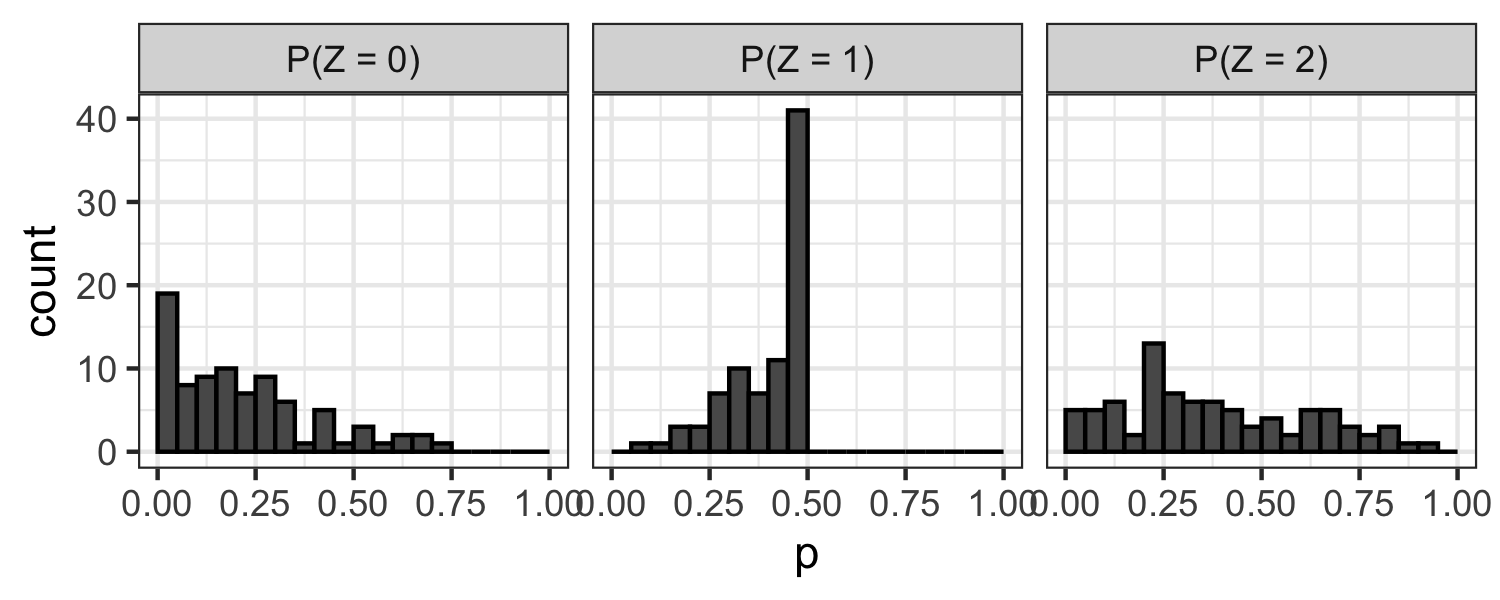
\includegraphics[width = \textwidth]{/Users/ralphtrane/Documents/RPackages_dev/ACEBounds/figures/example_analyses/smoking_lung_cancer_3_marginal_Z.png}
  \caption{Histograms of the marginal distribution of instruments, $P(Z = z), z=0,1,2$, estimated after preprocessing for analysis in Section \ref{smoking-effect-on-lung-cancer}.}
  \label{fig:marginal-distribution-of-instruments-lung-cancer}
\end{figure}

\begin{figure}[H]
  \center
  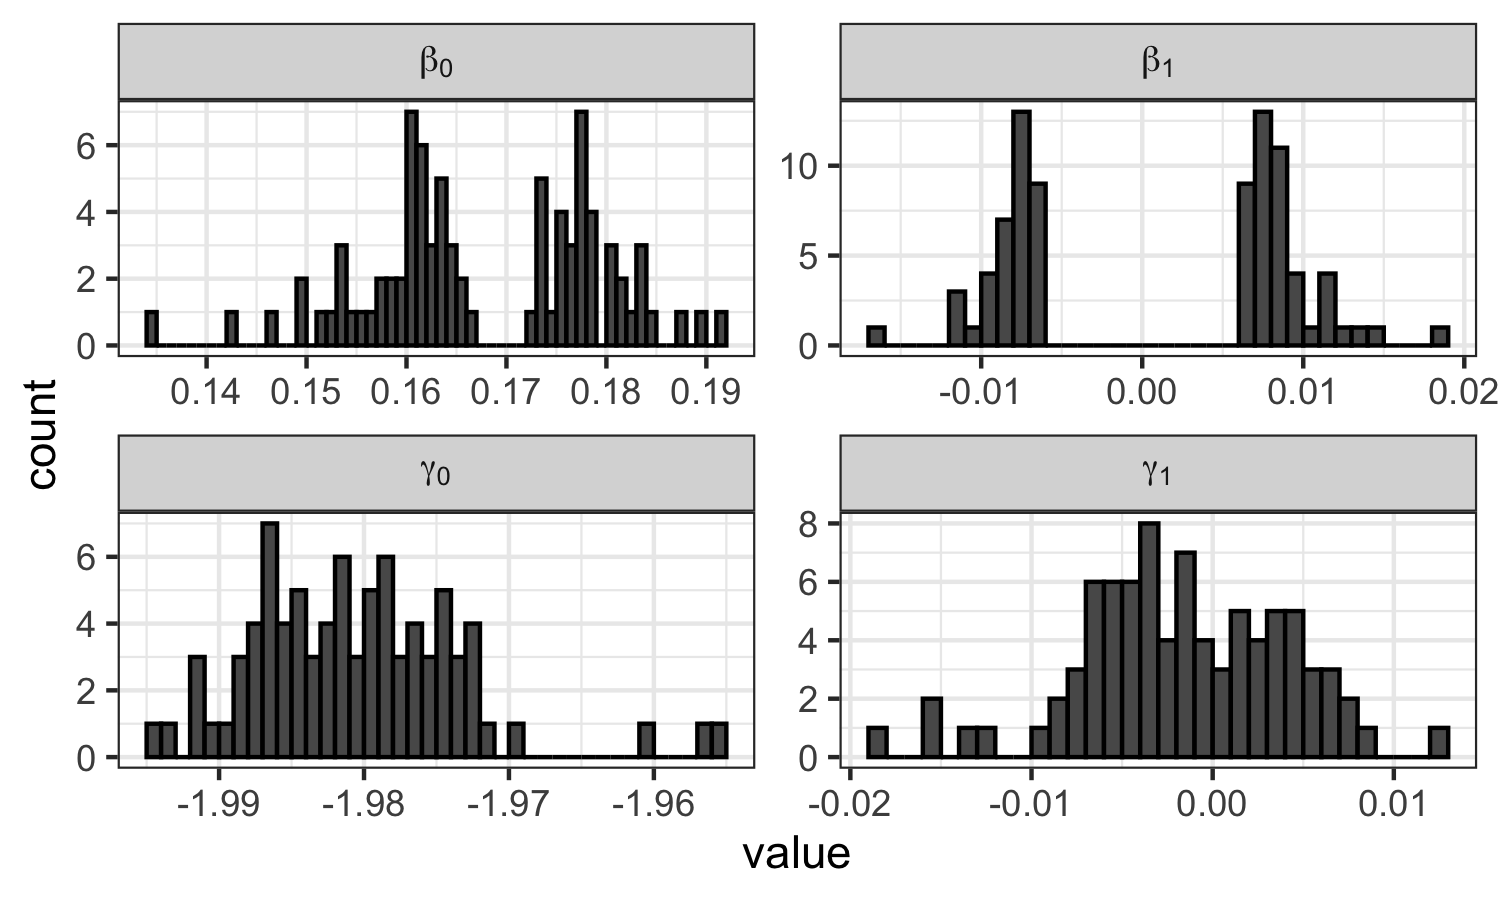
\includegraphics[width = \textwidth]{/Users/ralphtrane/Documents/RPackages_dev/ACEBounds/figures/example_analyses/smoking_lung_cancer_3_coefficients.png}
  \caption{Histograms of the coefficients from GWAS results of logistic regression of the SNPs on smoking status and lung cancer status. Intercepts ($\beta_0$ and $\gamma_0$) are inferred, while slopes ($\beta_1$ and $\gamma_1$) are as reported.}
  \label{fig:marginal-distribution-of-coefficients-lung-cancer}
\end{figure}

\begin{longtable}[t]{lrrrr}
\caption{\label{tab:coefficients-lung-cancer}Coefficients from GWAS results of logistic regression of the SNPs on smoking status and lung cancer status. Intercepts ($\beta_0$ and $\gamma_0$) are inferred, while slopes ($\beta_1$ and $\gamma_1$) are as reported.}\\
\toprule
SNP & $\beta_1$ & $\beta_0$ & $\gamma_1$ & $\gamma_0$\\
\midrule
\endfirsthead
\caption[]{\label{tab:coefficients-lung-cancer}Coefficients from GWAS results of logistic regression of the SNPs on smoking status and lung cancer status. Intercepts ($\beta_0$ and $\gamma_0$) are inferred, while slopes ($\beta_1$ and $\gamma_1$) are as reported. \textit{(continued)}}\\
\toprule
SNP & $\beta_1$ & $\beta_0$ & $\gamma_1$ & $\gamma_0$\\
\midrule
\endhead

\endfoot
\bottomrule
\endlastfoot
rs10173733 & -0.0065148 & 0.1773766 & 0.0033363 & -1.987122\\
rs10193706 & -0.0117667 & 0.1807753 & -0.0015310 & -1.981684\\
rs10233018 & -0.0076551 & 0.1771914 & 0.0050495 & -1.988150\\
rs10274594 & 0.0078326 & 0.1617046 & -0.0015364 & -1.981589\\
rs1029986 & -0.0070208 & 0.1754303 & 0.0035498 & -1.986088\\
\addlinespace
rs10774625 & 0.0074868 & 0.1621777 & -0.0084158 & -1.974806\\
rs10813628 & -0.0068761 & 0.1762662 & 0.0051706 & -1.988156\\
rs10897561 & -0.0066917 & 0.1782117 & 0.0066835 & -1.991747\\
rs10905461 & 0.0072731 & 0.1658787 & -0.0058844 & -1.980131\\
rs10914684 & 0.0077356 & 0.1591408 & -0.0026047 & -1.979616\\
\addlinespace
rs10956808 & 0.0076247 & 0.1607905 & -0.0063546 & -1.975802\\
rs11103667 & -0.0086047 & 0.1835048 & 0.0063118 & -1.993343\\
rs11127913 & 0.0081801 & 0.1596256 & -0.0033969 & -1.978997\\
rs11429972 & 0.0083148 & 0.1640148 & -0.0096129 & -1.976695\\
rs11611651 & -0.0119868 & 0.1914724 & 0.0013059 & -1.985521\\
\addlinespace
rs11631530 & -0.0099863 & 0.1872160 & -0.0047887 & -1.974691\\
rs11646575 & -0.0082446 & 0.1788545 & 0.0012319 & -1.984521\\
rs11693702 & -0.0080254 & 0.1781679 & 0.0046224 & -1.988077\\
rs117435980 & -0.0092037 & 0.1849986 & -0.0054804 & -1.973970\\
rs12042107 & 0.0071759 & 0.1631404 & -0.0020557 & -1.981288\\
\addlinespace
rs12244388 & -0.0104344 & 0.1834505 & 0.0019355 & -1.985707\\
rs12450028 & -0.0070626 & 0.1788556 & -0.0024536 & -1.979923\\
rs12479064 & -0.0080362 & 0.1823251 & -0.0088600 & -1.969116\\
rs12487411 & 0.0075048 & 0.1616745 & -0.0077980 & -1.974913\\
rs12608052 & 0.0067542 & 0.1631129 & -0.0048100 & -1.978521\\
\addlinespace
rs12725407 & 0.0081386 & 0.1564297 & -0.0067998 & -1.972138\\
rs12886628 & -0.0071010 & 0.1743626 & -0.0018595 & -1.981891\\
rs12910916 & -0.0090138 & 0.1838027 & 0.0026458 & -1.987308\\
rs13100688 & 0.0072663 & 0.1604864 & -0.0055464 & -1.976186\\
rs1492546 & -0.0068801 & 0.1757890 & 0.0040638 & -1.986797\\
\addlinespace
rs1499982 & -0.0114648 & 0.1730098 & 0.0024892 & -1.983878\\
rs1549213 & 0.0085270 & 0.1634849 & 0.0056335 & -1.987184\\
rs1561195 & -0.0078947 & 0.1771393 & 0.0072232 & -1.990046\\
rs1565735 & 0.0115901 & 0.1510915 & -0.0072487 & -1.971566\\
rs16951001 & -0.0066035 & 0.1772784 & 0.0070226 & -1.991313\\
\addlinespace
rs17003752 & 0.0098606 & 0.1526117 & -0.0055424 & -1.973591\\
rs17151637 & 0.0075112 & 0.1588020 & -0.0027771 & -1.979146\\
rs1899896 & -0.0079928 & 0.1808293 & 0.0047935 & -1.989876\\
rs2240294 & 0.0069566 & 0.1618616 & -0.0078381 & -1.974429\\
rs2416770 & -0.0064888 & 0.1756858 & -0.0035668 & -1.979794\\
\addlinespace
rs264974 & 0.0093111 & 0.1600323 & -0.0047198 & -1.978291\\
rs2675609 & 0.0081586 & 0.1635228 & -0.0069708 & -1.977953\\
rs2797116 & 0.0079136 & 0.1580011 & -0.0039635 & -1.977330\\
rs2867749 & 0.0069446 & 0.1601396 & -0.0032894 & -1.978658\\
rs299688 & -0.0072721 & 0.1737306 & -0.0019058 & -1.982055\\
\addlinespace
rs326341 & 0.0065809 & 0.1627032 & 0.0031753 & -1.986468\\
rs35891966 & 0.0147752 & 0.1421811 & -0.0122161 & -1.960473\\
rs379525 & -0.0064906 & 0.1763327 & -0.0018594 & -1.981209\\
rs42417 & -0.0070331 & 0.1739582 & 0.0003829 & -1.983375\\
rs4566215 & 0.0066219 & 0.1634100 & -0.0035546 & -1.979817\\
\addlinespace
rs4910656 & 0.0068438 & 0.1605890 & -0.0006962 & -1.982221\\
rs4957528 & -0.0084750 & 0.1731252 & 0.0036288 & -1.984649\\
rs523528 & 0.0080708 & 0.1629116 & 0.0029251 & -1.985564\\
rs528301 & -0.0086008 & 0.1773068 & 0.0124616 & -1.994333\\
rs55921136 & 0.0085950 & 0.1559000 & -0.0069653 & -1.972040\\
\addlinespace
rs568599 & -0.0067027 & 0.1757286 & 0.0043346 & -1.987105\\
rs5850689 & 0.0119733 & 0.1608296 & -0.0038879 & -1.980291\\
rs60745548 & 0.0071946 & 0.1656670 & 0.0062353 & -1.986552\\
rs6141314 & -0.0080616 & 0.1818108 & 0.0010534 & -1.984733\\
rs6265 & 0.0101598 & 0.1531146 & -0.0043806 & -1.976031\\
\addlinespace
rs6433897 & -0.0072353 & 0.1734104 & -0.0011588 & -1.982527\\
rs6676022 & 0.0115926 & 0.1492373 & -0.0153059 & -1.956268\\
rs6690680 & 0.0088409 & 0.1547067 & -0.0050219 & -1.974679\\
rs6828849 & 0.0067122 & 0.1617773 & 0.0008050 & -1.984076\\
rs71550128 & -0.0073950 & 0.1762278 & 0.0034139 & -1.986200\\
\addlinespace
rs72505558 & 0.0067437 & 0.1614885 & -0.0009876 & -1.981950\\
rs72678864 & 0.0097538 & 0.1534836 & -0.0034394 & -1.977455\\
rs7333559 & 0.0080523 & 0.1662222 & -0.0183846 & -1.975467\\
rs7451586 & -0.0066732 & 0.1775422 & 0.0027432 & -1.986404\\
rs748828 & 0.0086213 & 0.1572389 & -0.0047229 & -1.976368\\
\addlinespace
rs7528604 & 0.0068658 & 0.1618157 & -0.0001820 & -1.982931\\
rs7567570 & -0.0091324 & 0.1727617 & -0.0002451 & -1.983053\\
rs763053 & 0.0080618 & 0.1570972 & -0.0069210 & -1.972409\\
rs76608582 & 0.0182891 & 0.1347646 & -0.0048192 & -1.973958\\
rs772921 & 0.0072725 & 0.1600453 & -0.0054837 & -1.975937\\
\addlinespace
rs77878475 & 0.0125950 & 0.1465726 & 0.0010985 & -1.985146\\
rs7870475 & -0.0071900 & 0.1771594 & 0.0082598 & -1.991835\\
rs7948789 & -0.0161713 & 0.1894568 & 0.0009336 & -1.984284\\
rs883403 & 0.0094240 & 0.1536556 & -0.0014726 & -1.980646\\
rs9375371 & -0.0073963 & 0.1804155 & -0.0069852 & -1.972929\\
\addlinespace
rs9381917 & 0.0112569 & 0.1493838 & -0.0155636 & -1.955201\\
rs9423279 & 0.0076695 & 0.1643324 & 0.0046716 & -1.986350\\
rs9487626 & 0.0131029 & 0.1648247 & -0.0136868 & -1.978168\\
rs9835772 & -0.0078024 & 0.1814198 & -0.0031275 & -1.978401\\*
\end{longtable}

\begin{figure}[H]
 \center
 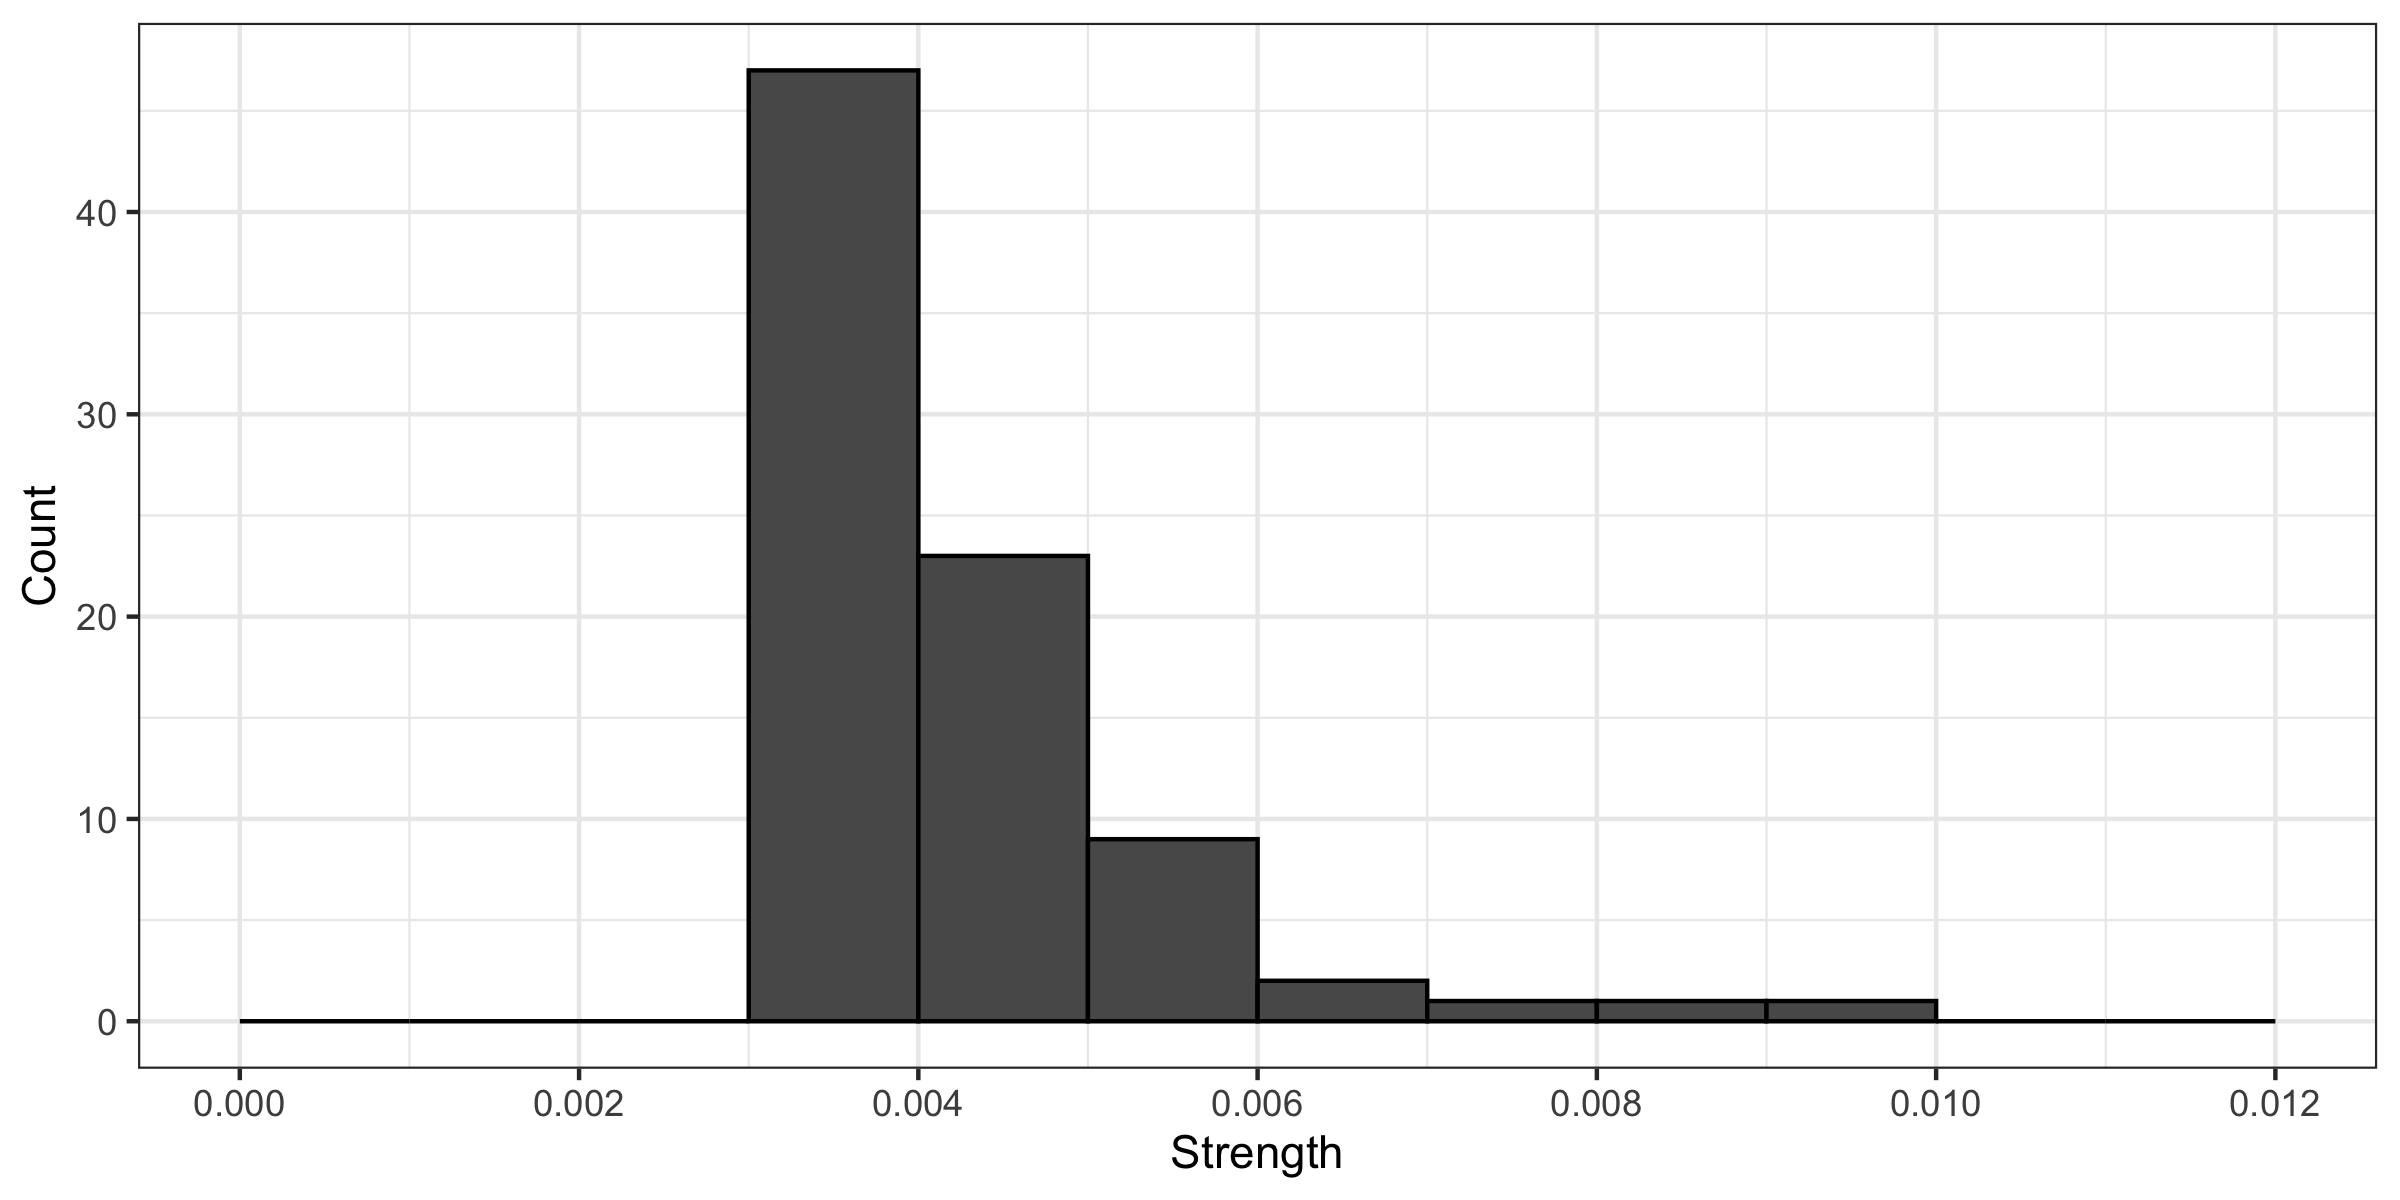
\includegraphics[width = 0.99\linewidth]{/Users/ralphtrane/Documents/RPackages_dev/ACEBounds/figures/example_analyses/strength_histogram.png}
 \caption{Histogram of strengths of IVs on the exposure. Here, SNPs are IVs, and smoking status (ever/never) is exposure. We see that all IVs are very weak, with the largest value just below 0.01.}
 \label{fig:strength_histogram}
\end{figure}

\begin{figure}[H]
  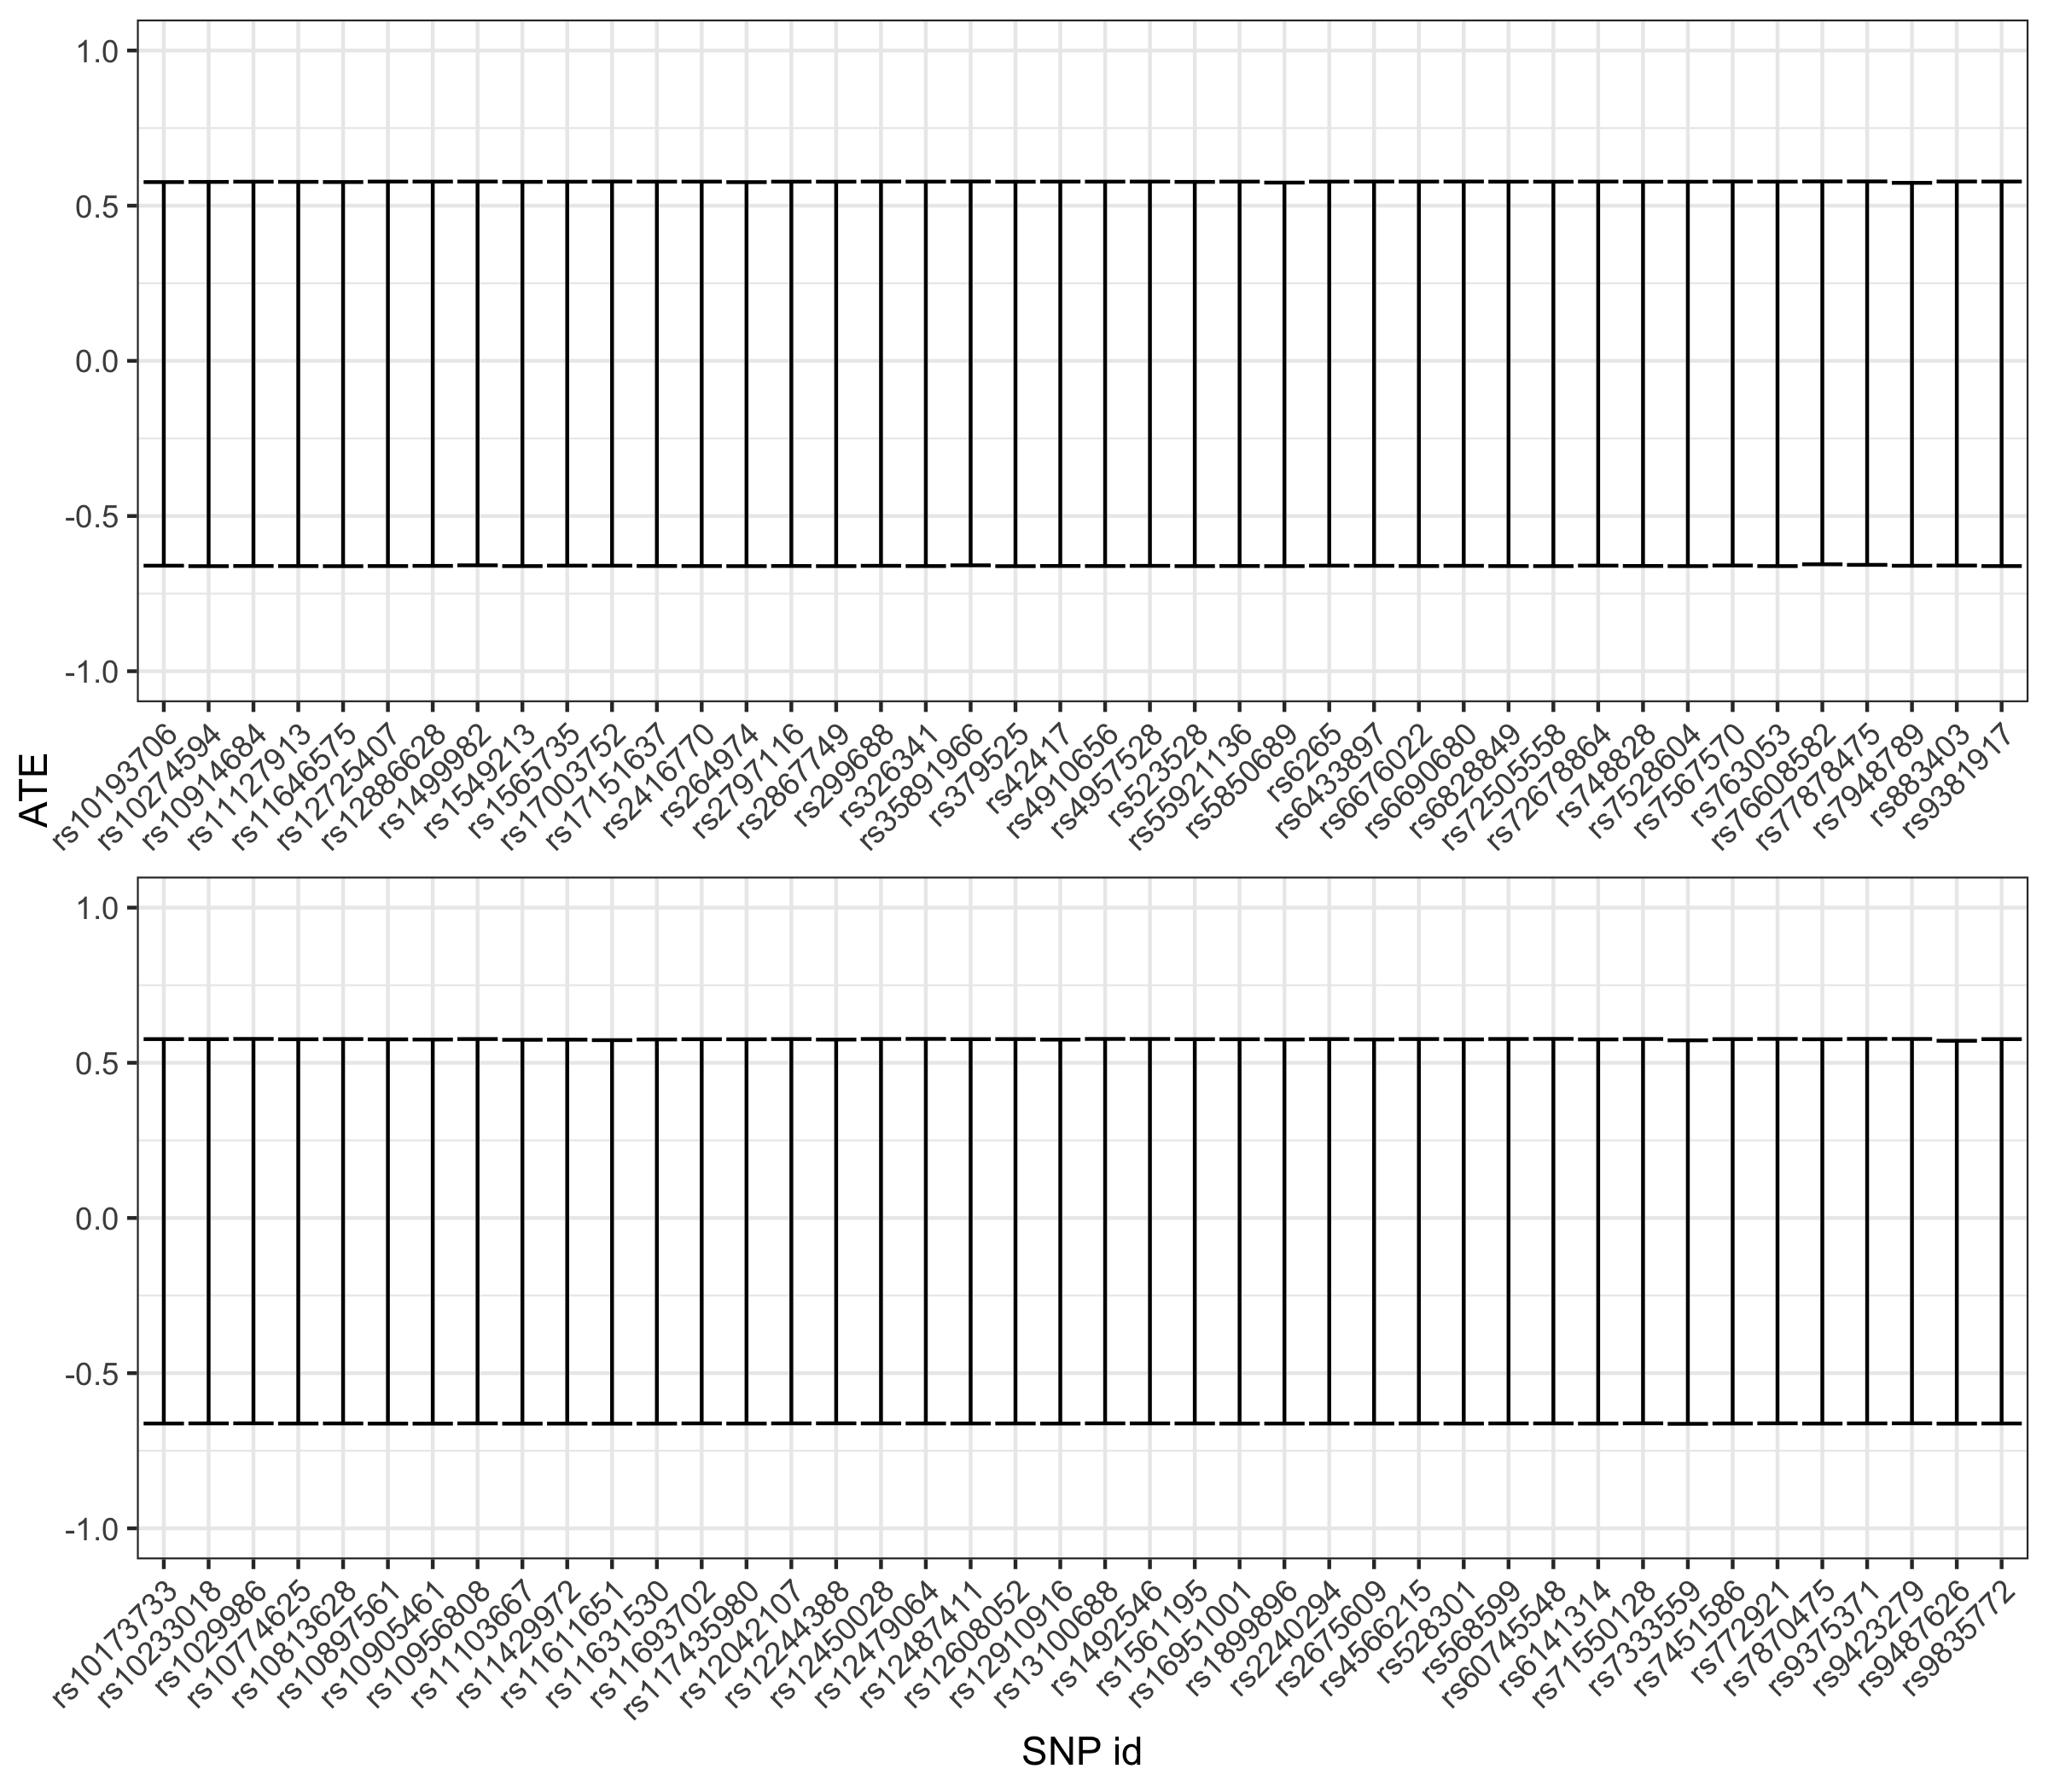
\includegraphics[width = 0.99\linewidth]{/Users/ralphtrane/Documents/RPackages_dev/ACEBounds/figures/example_analyses/smoking_lung_cancer_3_bivaraite_bounds_ukb-d-20116_0_ukb-d-40001_C349.png}
  \caption{Nonparametric two-sample IV bounds on the average treatment effect of smoking on the incidence of lung cancer.}
  \label{fig:smoking_on_lung_cancer_ind_bounds}
\end{figure}

\begin{figure}[H]
  \center
  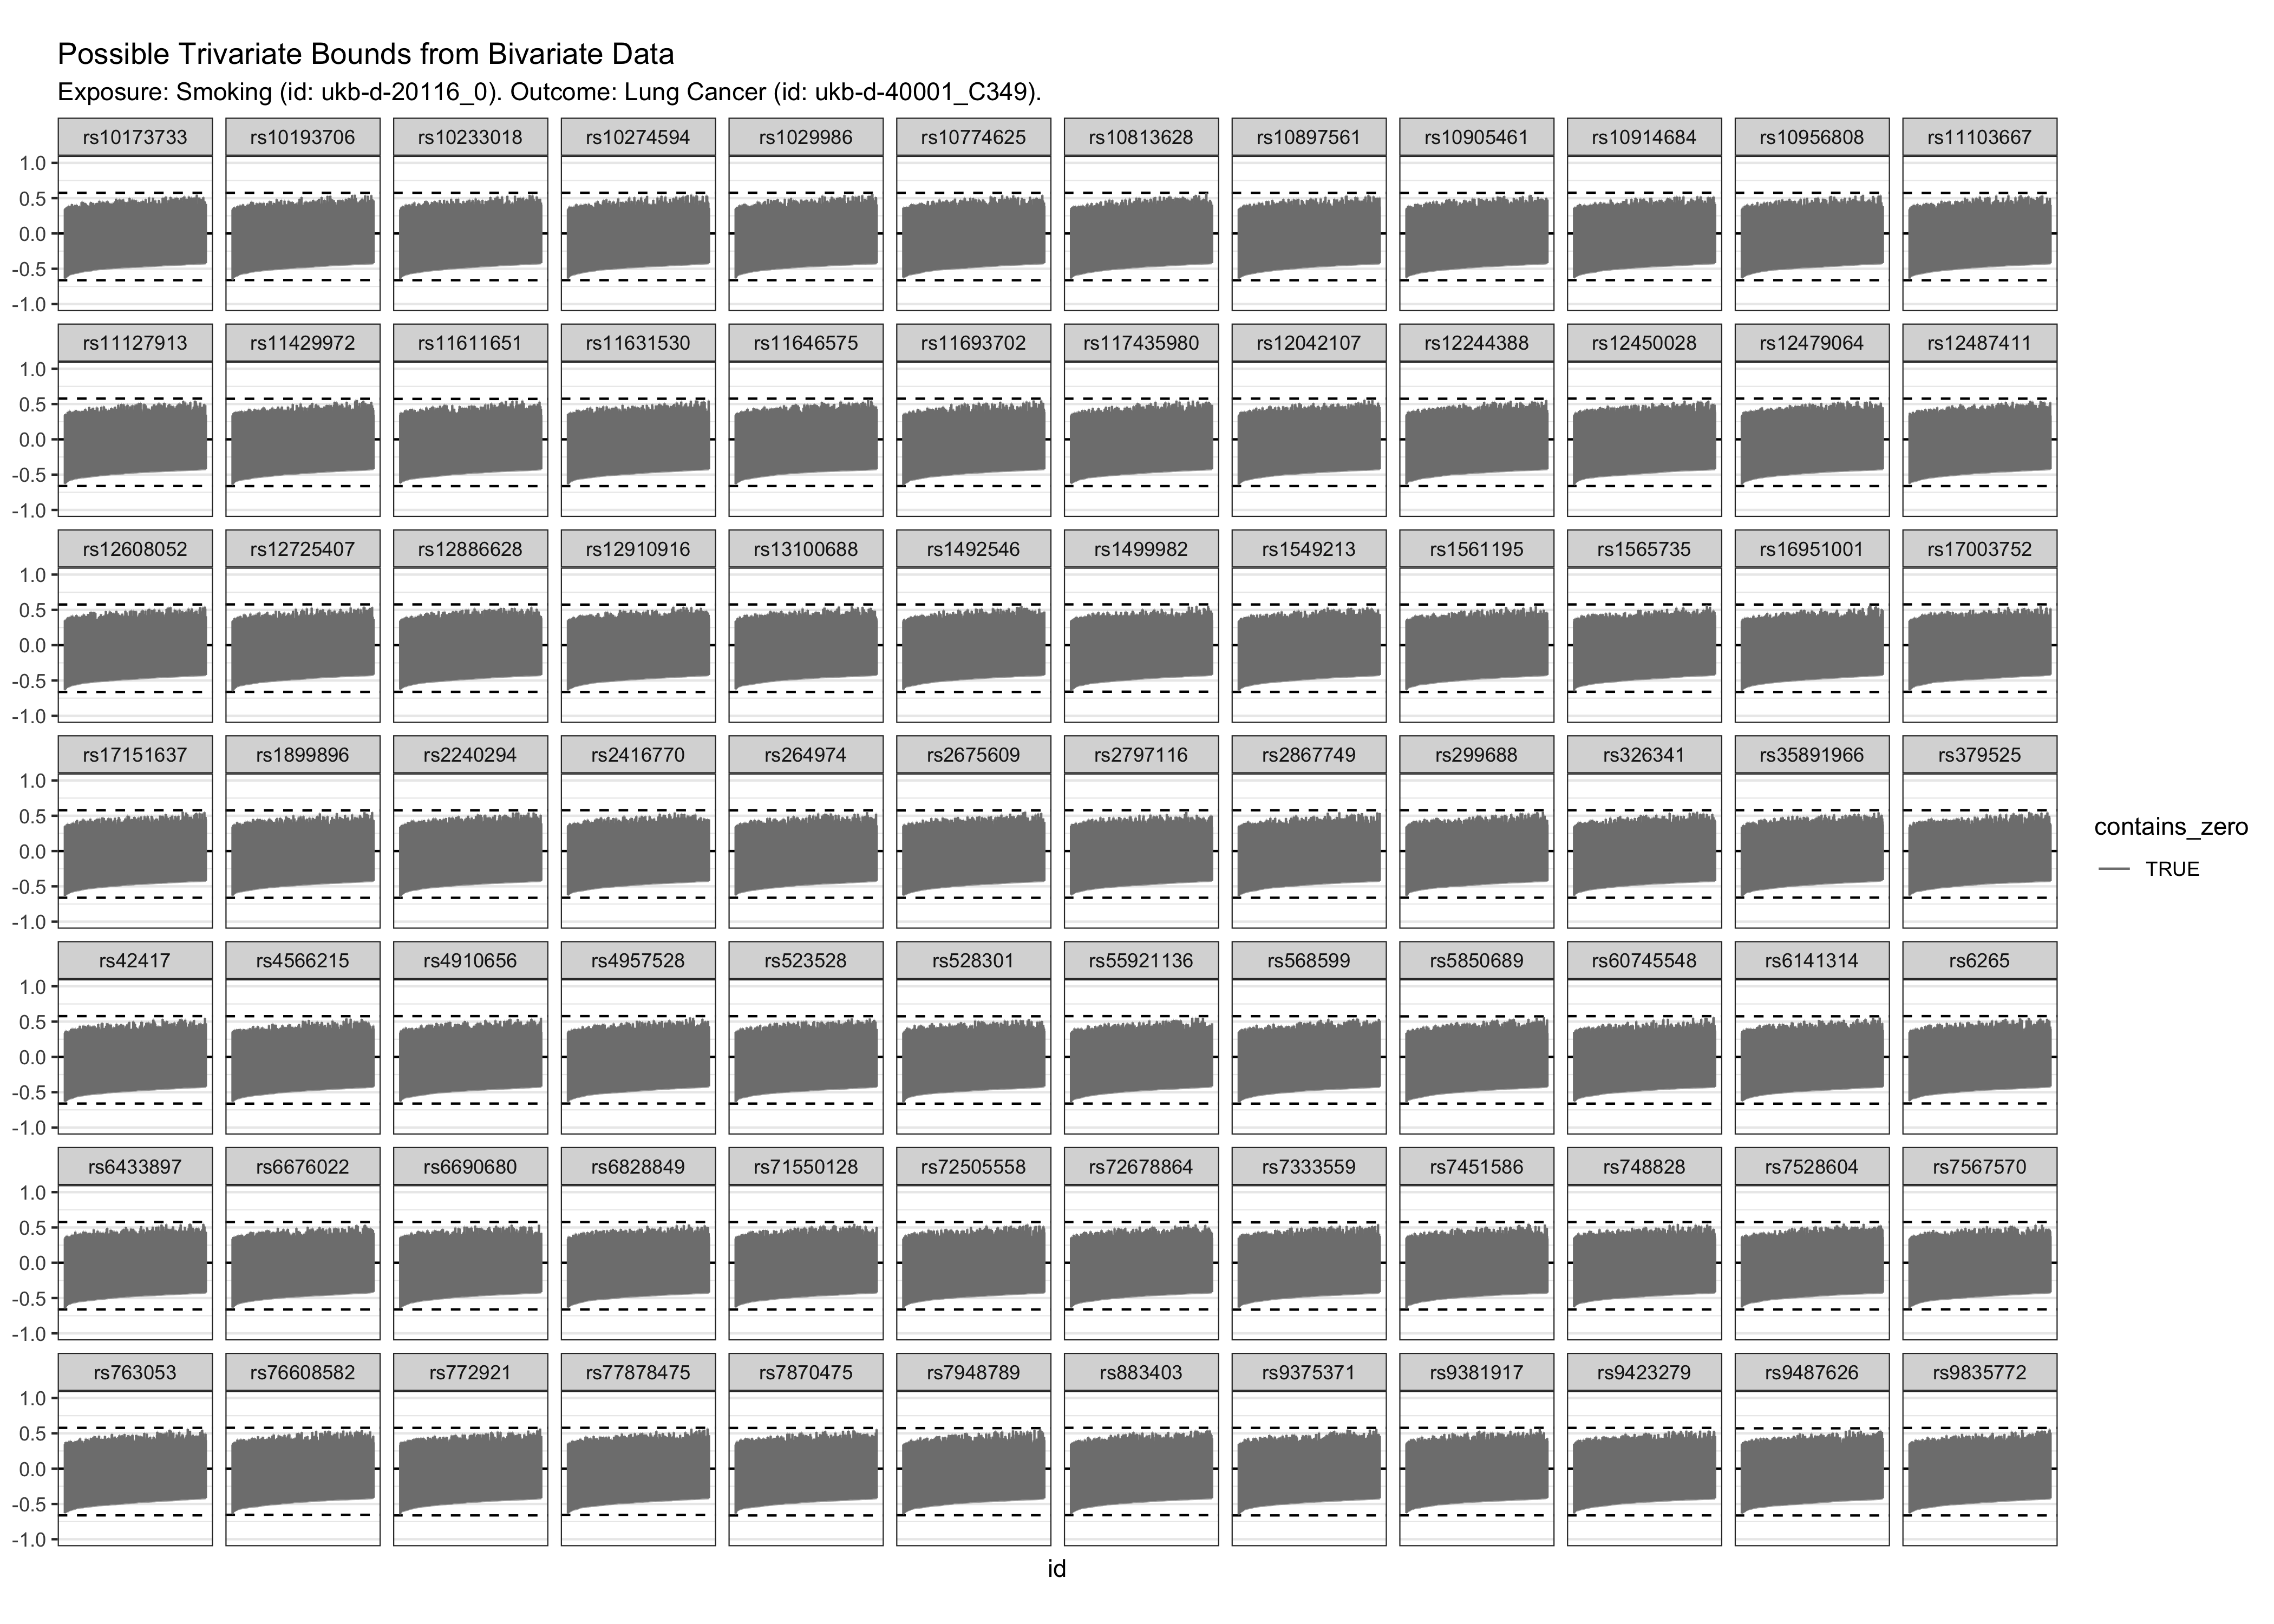
\includegraphics[width = 0.99\textwidth]{/Users/ralphtrane/Documents/RPackages_dev/ACEBounds/figures/example_analyses/smoking_lung_cancer_3_individual_SNPs_plot_ukb-d-20116_0_ukb-d-40001_C349.png}
    \caption{500 sets of bounds of the average treatment effect of smoking on lung cancer for each of the 84 SNPs. Each bound is based on a set of values for the trivariate distribution randomly sampled. Bounds are color coded to show if they overlap 0 (grey) or do not (red). All bounds overlap 0.}
    \label{fig:smoking_on_lung_cancer_tri_bounds_all}
\end{figure}

\begin{figure}[H]
  \center
  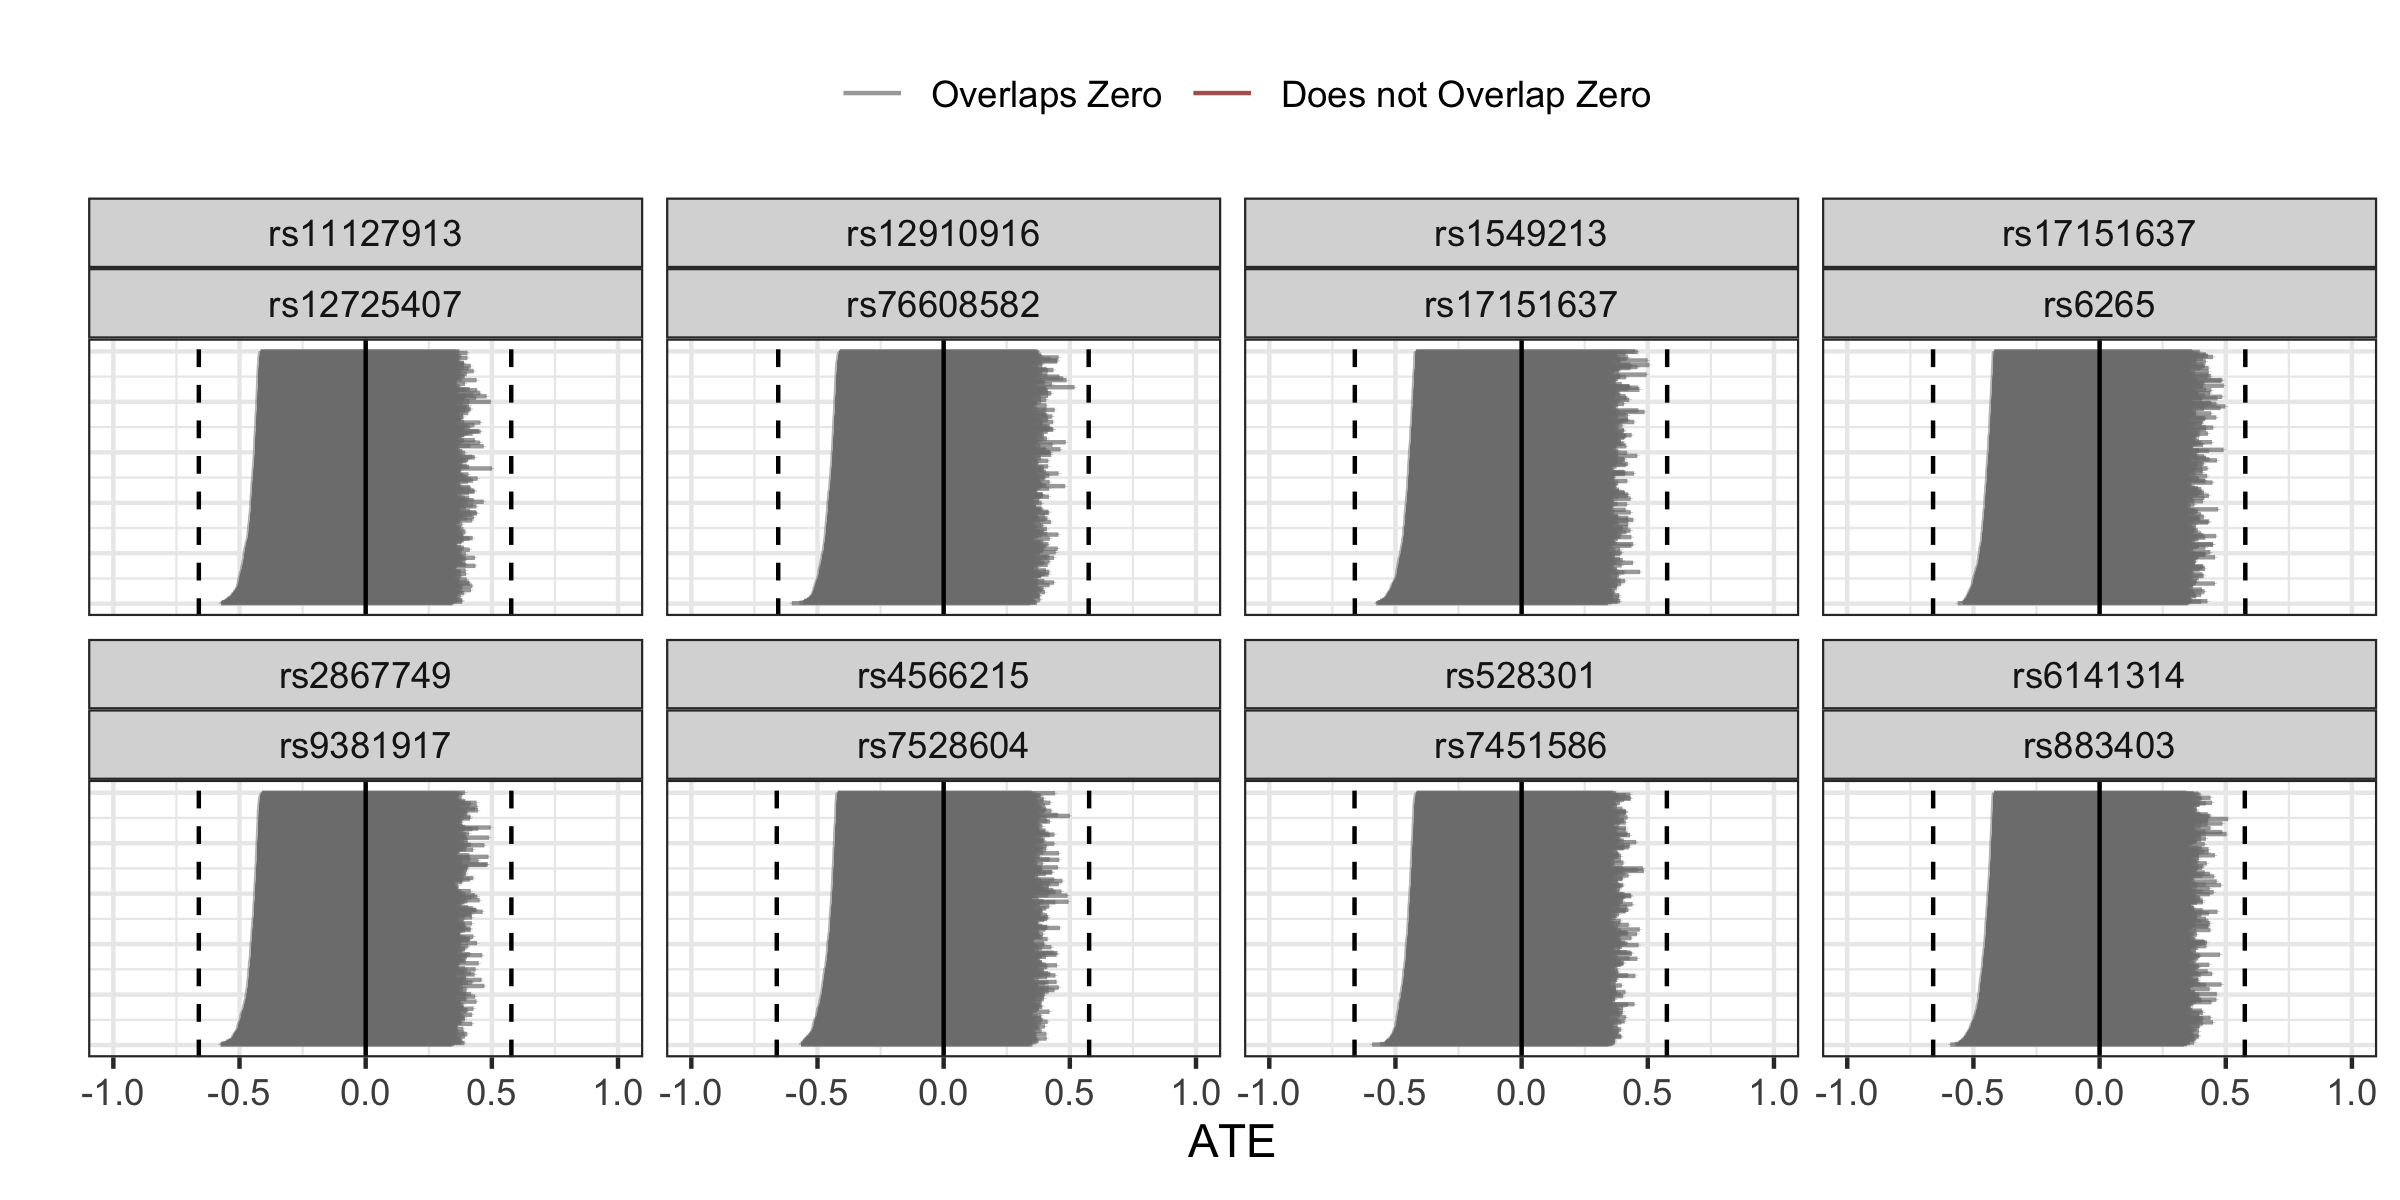
\includegraphics[width = 0.99\linewidth]{/Users/ralphtrane/Documents/RPackages_dev/ACEBounds/figures/example_analyses/smoking_lung_cancer_3_intersection_bounds_plot_ukb-d-20116_0_ukb-d-40001_C349.png}
  \caption{Intersection bounds of the average treatment effect of smoking on lung cancer based on randomly sampled trivariate distributions from pairs of SNPs. These 8 pairs were randomly chosen from all possible pairs.}
  \label{fig:smoking_on_lung_cancer_intersections}
\end{figure}

\hypertarget{effect-of-high-cholesterol-on-heart-attack}{%
\subsection{\texorpdfstring{Effect of High Cholesterol on Heart Attack \label{appendix:cholesterol-on-heart-attack}}{Effect of High Cholesterol on Heart Attack }}\label{effect-of-high-cholesterol-on-heart-attack}}

\begin{figure}[H]
  \center
  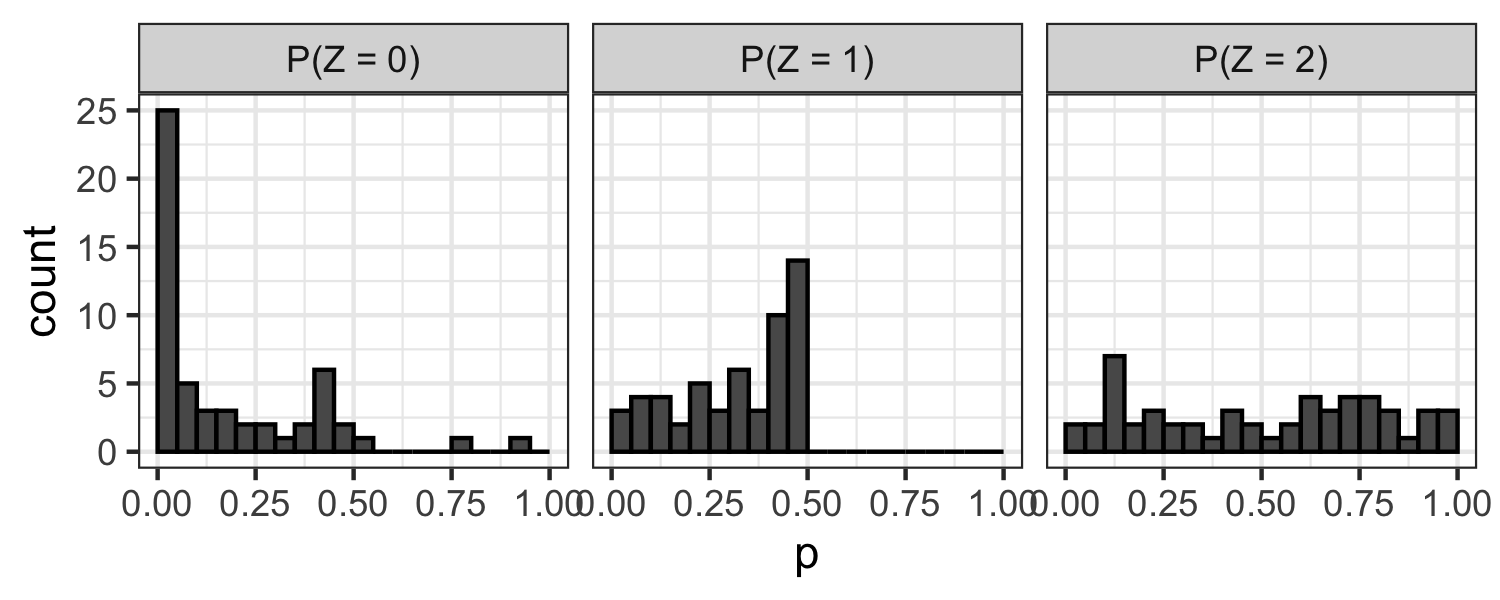
\includegraphics[width = \textwidth]{/Users/ralphtrane/Documents/RPackages_dev/ACEBounds/figures/example_analyses/cholesterol_heart_attack_marginal_Z.png}
  \caption{Histograms of the marginal distribution of instruments, $P(Z = z), z=0,1,2$, estimated after preprocessing for analysis in Section \ref{cholesterol-on-heart-attack}}
  \label{fig:marginal-distribution-of-instruments-cholesterol-heart-attack}
\end{figure}

\begin{table}[H]
  \caption{Table of the marginal distribution of instruments, $P(Z = z), z=0,1,2$, estimated after preprocessing for analysis in Section \ref{cholesterol-on-heart-attack}}
  \label{tab:marginal-distribution-of-instruments-lung-cancer}
  \begin{minipage}{0.5\linewidth}
    \center
    
\begin{tabular}{lrrr}
\toprule
SNP & P(Z = 2) & P(Z = 1) & P(Z = 0)\\
\midrule
rs10096633 & 0.7682873 & 0.2164654 & 0.0152473\\
rs10260606 & 0.6689457 & 0.2978906 & 0.0331637\\
rs10410835 & 0.2261041 & 0.4987999 & 0.2750961\\
rs10504255 & 0.1141345 & 0.4474070 & 0.4384585\\
rs10804330 & 0.3246447 & 0.4902626 & 0.1850927\\
\addlinespace
rs112019714 & 0.9445278 & 0.0546808 & 0.0007914\\
rs11580878 & 0.2532012 & 0.4999796 & 0.2468192\\
rs11591147 & 0.9653935 & 0.0343018 & 0.0003047\\
rs117733303 & 0.9629825 & 0.0366685 & 0.0003491\\
rs12471811 & 0.7974669 & 0.1910863 & 0.0114469\\
\addlinespace
rs1260326 & 0.1542518 & 0.4769944 & 0.3687538\\
rs12740374 & 0.6060342 & 0.3448956 & 0.0490702\\
rs12916 & 0.3593703 & 0.4802094 & 0.1604203\\
rs1367117 & 0.4370916 & 0.4480749 & 0.1148336\\
rs1601935 & 0.1186871 & 0.4516457 & 0.4296671\\
\addlinespace
rs1883025 & 0.5579089 & 0.3780482 & 0.0640429\\
rs1883711 & 0.9385769 & 0.0604497 & 0.0009733\\
rs2125345 & 0.4990744 & 0.4147551 & 0.0861704\\
rs2237107 & 0.6333104 & 0.3249953 & 0.0416944\\
rs2244608 & 0.4686429 & 0.4318641 & 0.0994929\\
\addlinespace
rs2618567 & 0.1161249 & 0.4492923 & 0.4345829\\
rs2738447 & 0.1661712 & 0.4829396 & 0.3508892\\
rs28601761 & 0.3342690 & 0.4877820 & 0.1779490\\
rs28807203 & 0.9046336 & 0.0929773 & 0.0023890\\
rs3127580 & 0.7081492 & 0.2667336 & 0.0251172\\
\addlinespace
rs34042070 & 0.6625016 & 0.3028808 & 0.0346176\\
rs34707604 & 0.5518930 & 0.3820040 & 0.0661030\\
\bottomrule
\end{tabular}


  \end{minipage}
  \qquad
  \begin{minipage}{0.5\linewidth}
    \center
    
\begin{tabular}{lrrr}
\toprule
SNP & P(Z = 2) & P(Z = 1) & P(Z = 0)\\
\midrule
rs3918226 & 0.8434773 & 0.1498658 & 0.0066569\\
rs4299376 & 0.1044835 & 0.4375111 & 0.4580055\\
rs4470903 & 0.6122421 & 0.3404338 & 0.0473241\\
rs456598 & 0.7353800 & 0.2443260 & 0.0202940\\
rs4704727 & 0.1153479 & 0.4485623 & 0.4360899\\
\addlinespace
rs472495 & 0.1219232 & 0.4545036 & 0.4235732\\
rs56299331 & 0.6368870 & 0.3223300 & 0.0407830\\
rs57180587 & 0.7289642 & 0.2496596 & 0.0213762\\
rs58542926 & 0.8541959 & 0.1400626 & 0.0057415\\
rs58691354 & 0.7129641 & 0.2628159 & 0.0242201\\
\addlinespace
rs59950280 & 0.4469685 & 0.4431771 & 0.1098545\\
rs6090040 & 0.2300488 & 0.4991705 & 0.2707808\\
rs622871 & 0.0988228 & 0.4310763 & 0.4701008\\
rs635634 & 0.6627002 & 0.3027276 & 0.0345722\\
rs6458349 & 0.0768498 & 0.4007364 & 0.5224138\\
\addlinespace
rs6511720 & 0.7764852 & 0.2093975 & 0.0141172\\
rs7012637 & 0.2755284 & 0.4987592 & 0.2257124\\
rs7213086 & 0.2001050 & 0.4944520 & 0.3054430\\
rs73534263 & 0.7971401 & 0.1913739 & 0.0114861\\
rs7412 & 0.8445834 & 0.1488576 & 0.0065590\\
\addlinespace
rs74617384 & 0.8447171 & 0.1487357 & 0.0065473\\
rs7534572 & 0.1255675 & 0.4575751 & 0.4168575\\
rs7707394 & 0.4169078 & 0.4575523 & 0.1255398\\
rs77542162 & 0.9546715 & 0.0448029 & 0.0005257\\
rs799157 & 0.0018869 & 0.0831041 & 0.9150089\\
\addlinespace
rs9376091 & 0.5451282 & 0.3863995 & 0.0684722\\
rs964184 & 0.0174433 & 0.2292594 & 0.7532973\\
\bottomrule
\end{tabular}


  \end{minipage}
\end{table}

\begin{figure}[H]
  \center
  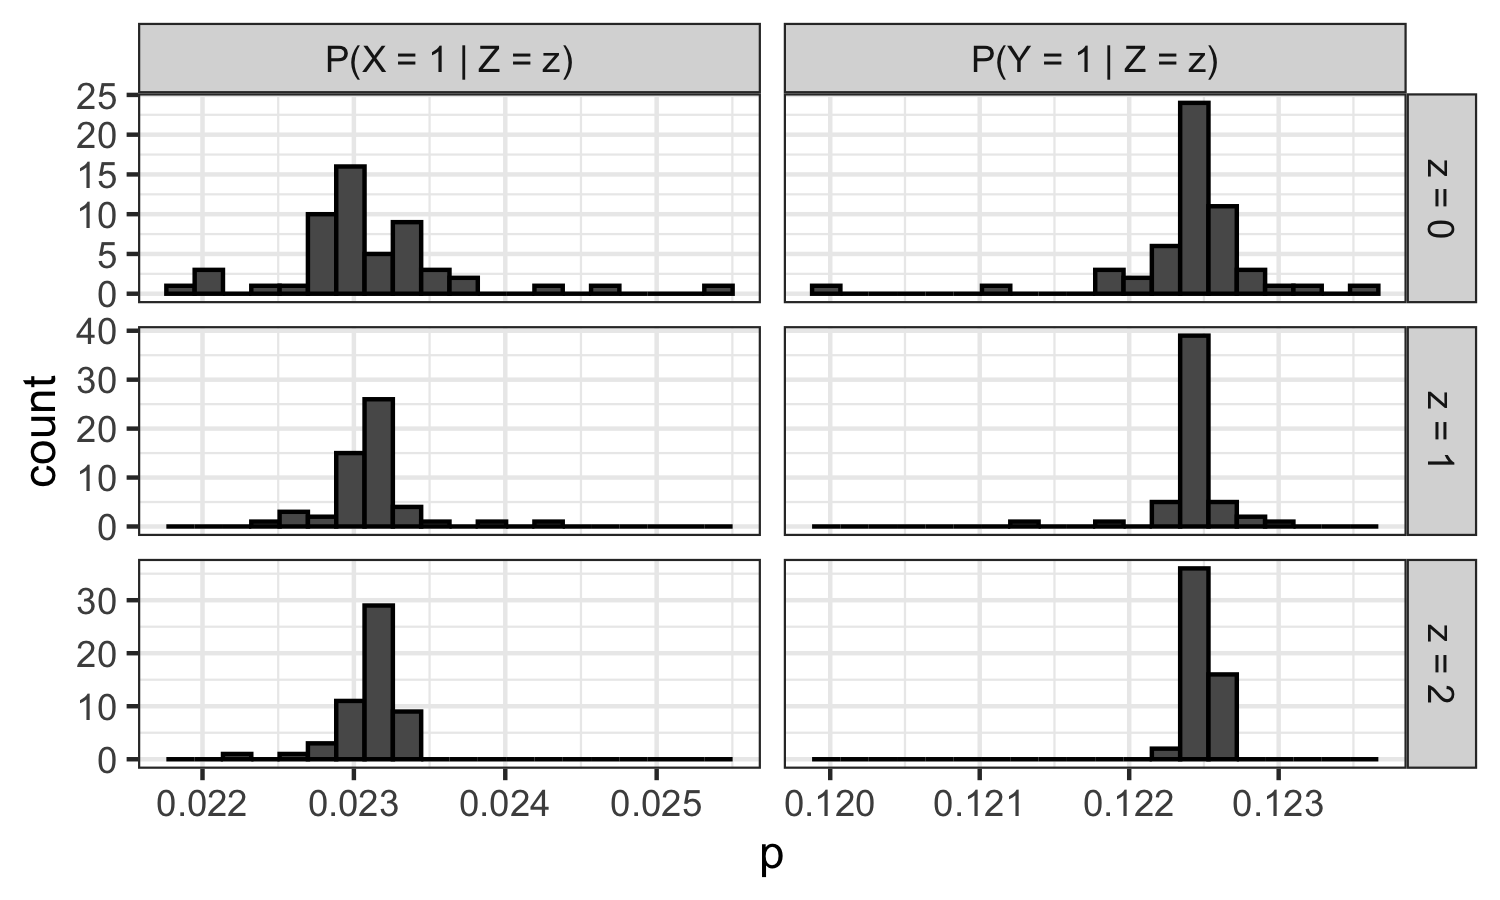
\includegraphics[width = 0.99\linewidth]{/Users/ralphtrane/Documents/RPackages_dev/ACEBounds/figures/example_analyses/cholesterol_heart_attack_marginal_conditionals.png}
  \caption{Histograms of the marginal conditional probabilities $P(X = 1 | Z = z), z = 0,1,2$ and $P(Y = 1 | Z = z), z=0,1,2$.}
  \label{fig:smoking_on_depression_marginals}
\end{figure}

\begin{figure}[H]
  \center
  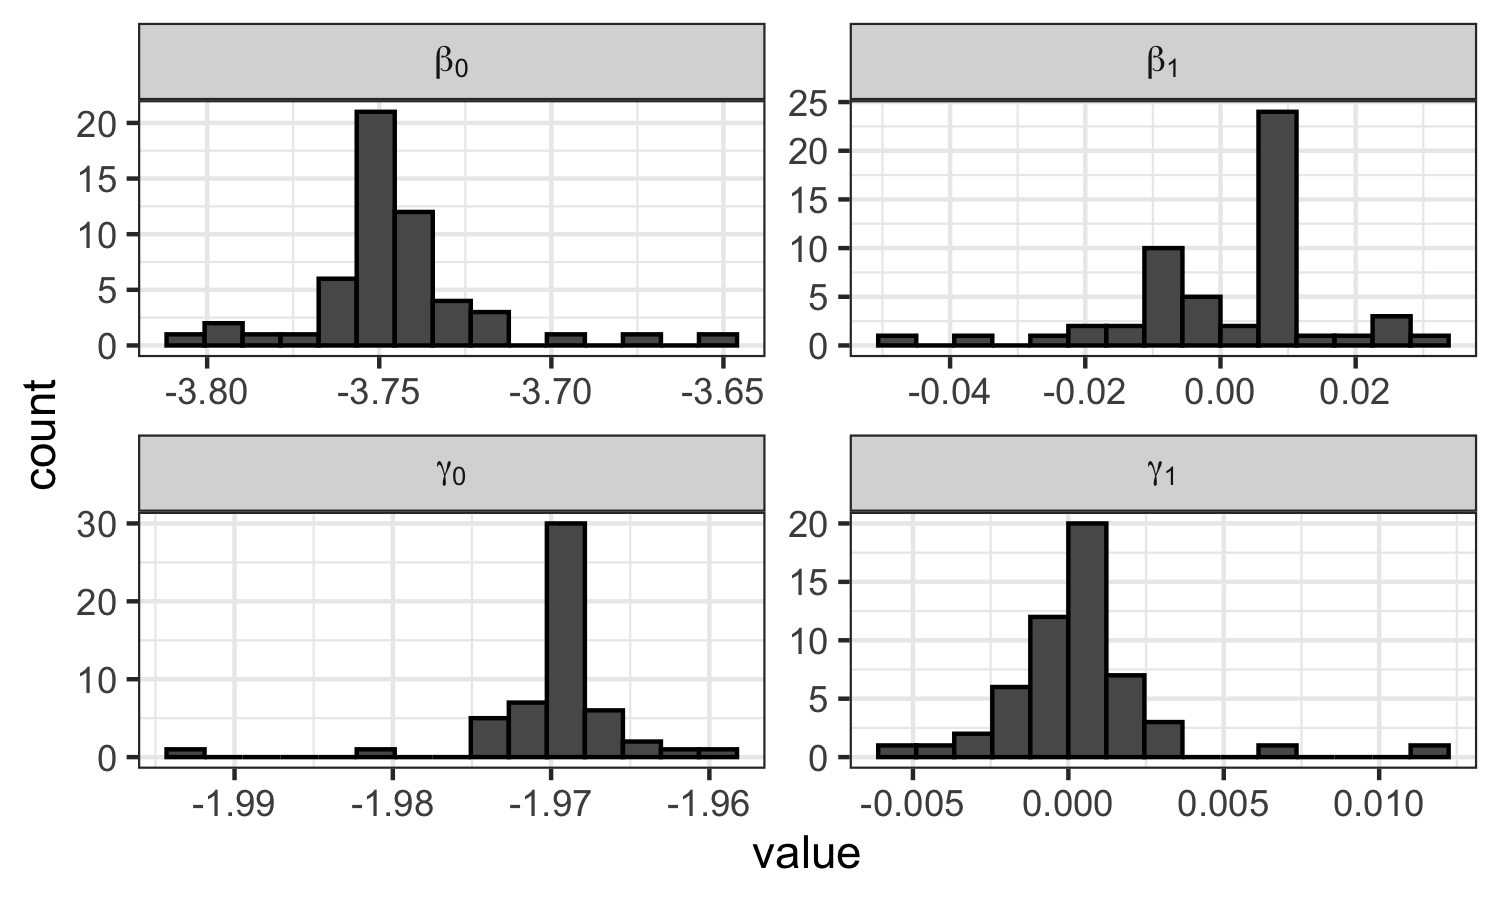
\includegraphics[width = \textwidth]{/Users/ralphtrane/Documents/RPackages_dev/ACEBounds/figures/example_analyses/cholesterol_heart_attack_coefficients.png}
  \caption{Histograms of the coefficients from GWAS results of logistic regression of the SNPs on high cholesterol and heart attack, respectively. Intercepts ($\beta_0$ and $\gamma_0$) are inferred, while slopes ($\beta_1$ and $\gamma_1$) are as reported.}
  \label{fig:marginal-distribution-of-coefficients-depression}
\end{figure}

\begin{longtable}[t]{lrrrr}
\caption{\label{tab:coefficients-cholesterol}Coefficients from GWAS results of logistic regression of the SNPs on high cholesterol and heart attack status. Intercepts ($\beta_0$ and $\gamma_0$) are inferred, while slopes ($\beta_1$ and $\gamma_1$) are as reported.}\\
\toprule
SNP & $\beta_1$ & $\beta_0$ & $\gamma_1$ & $\gamma_0$\\
\midrule
\endfirsthead
\caption[]{\label{tab:coefficients-cholesterol}Coefficients from GWAS results of logistic regression of the SNPs on high cholesterol and heart attack status. Intercepts ($\beta_0$ and $\gamma_0$) are inferred, while slopes ($\beta_1$ and $\gamma_1$) are as reported. \textit{(continued)}}\\
\toprule
SNP & $\beta_1$ & $\beta_0$ & $\gamma_1$ & $\gamma_0$\\
\midrule
\endhead

\endfoot
\bottomrule
\endlastfoot
rs10096633 & -0.0089830 & -3.727152 & -0.0012995 & -1.966860\\
rs10260606 & 0.0076950 & -3.755485 & 0.0007029 & -1.970288\\
rs10410835 & 0.0071078 & -3.749661 & 0.0007948 & -1.969894\\
rs10504255 & -0.0056764 & -3.739063 & -0.0000742 & -1.969088\\
rs10804330 & -0.0050169 & -3.737181 & -0.0012539 & -1.967709\\
\addlinespace
rs112019714 & 0.0251675 & -3.791824 & 0.0025525 & -1.974100\\
rs11580878 & -0.0051399 & -3.737725 & -0.0006621 & -1.968472\\
rs11591147 & -0.0476105 & -3.649365 & -0.0054389 & -1.958449\\
rs117733303 & 0.0311528 & -3.804047 & 0.0116909 & -1.992088\\
rs12471811 & 0.0084776 & -3.758037 & 0.0000048 & -1.969147\\
\addlinespace
rs1260326 & -0.0102312 & -3.734879 & -0.0003941 & -1.968828\\
rs12740374 & -0.0183231 & -3.714419 & -0.0025251 & -1.965207\\
rs12916 & 0.0104793 & -3.755479 & 0.0006700 & -1.969941\\
rs1367117 & 0.0155585 & -3.763513 & 0.0011495 & -1.970658\\
rs1601935 & -0.0061378 & -3.738671 & -0.0007014 & -1.968655\\
\addlinespace
rs1883025 & -0.0069826 & -3.732469 & -0.0013153 & -1.967173\\
rs1883711 & 0.0241076 & -3.789616 & 0.0026734 & -1.974319\\
rs2125345 & -0.0056374 & -3.734933 & -0.0009408 & -1.967809\\
rs2237107 & -0.0070166 & -3.731732 & -0.0007194 & -1.967993\\
rs2244608 & 0.0070205 & -3.752512 & 0.0010406 & -1.970563\\
\addlinespace
rs2618567 & -0.0047485 & -3.739660 & -0.0007455 & -1.968630\\
rs2738447 & 0.0081671 & -3.749563 & 0.0016947 & -1.970520\\
rs28601761 & -0.0140739 & -3.726664 & -0.0011169 & -1.967847\\
rs28807203 & -0.0106943 & -3.722554 & -0.0002164 & -1.968726\\
rs3127580 & 0.0076693 & -3.755804 & 0.0022978 & -1.973006\\
\addlinespace
rs34042070 & 0.0094413 & -3.758272 & 0.0002698 & -1.969577\\
rs34707604 & 0.0058521 & -3.751591 & 0.0002016 & -1.969438\\
rs3918226 & 0.0081783 & -3.757916 & 0.0028105 & -1.974301\\
rs4299376 & -0.0111342 & -3.735719 & -0.0012431 & -1.968335\\
rs4470903 & 0.0067035 & -3.753387 & 0.0014579 & -1.971420\\
\addlinespace
rs456598 & 0.0065720 & -3.754166 & 0.0005768 & -1.970127\\
rs4704727 & 0.0074887 & -3.747988 & 0.0007432 & -1.969643\\
rs472495 & 0.0064154 & -3.747379 & 0.0004743 & -1.969469\\
rs56299331 & 0.0057258 & -3.752033 & 0.0001068 & -1.969308\\
rs57180587 & 0.0081592 & -3.756830 & 0.0013685 & -1.971475\\
\addlinespace
rs58542926 & -0.0146353 & -3.715853 & -0.0013536 & -1.966636\\
rs58691354 & 0.0074756 & -3.755521 & 0.0000196 & -1.969171\\
rs59950280 & 0.0058286 & -3.750690 & 0.0004805 & -1.969780\\
rs6090040 & -0.0055812 & -3.737545 & -0.0007168 & -1.968450\\
rs622871 & 0.0065093 & -3.746991 & 0.0013161 & -1.969966\\
\addlinespace
rs635634 & 0.0098788 & -3.758987 & 0.0014151 & -1.971442\\
rs6458349 & 0.0056558 & -3.746031 & 0.0007529 & -1.969556\\
rs6511720 & -0.0261322 & -3.696906 & -0.0030216 & -1.963813\\
rs7012637 & 0.0047984 & -3.747932 & 0.0002456 & -1.969396\\
rs7213086 & 0.0047773 & -3.747169 & 0.0007846 & -1.969840\\
\addlinespace
rs73534263 & 0.0071810 & -3.755717 & 0.0000767 & -1.969275\\
rs7412 & -0.0374088 & -3.674234 & -0.0038000 & -1.962153\\
rs74617384 & 0.0190473 & -3.777927 & 0.0069894 & -1.981990\\
rs7534572 & 0.0081187 & -3.748658 & 0.0005830 & -1.969551\\
rs7707394 & 0.0061511 & -3.750841 & 0.0000817 & -1.969243\\
\addlinespace
rs77542162 & 0.0253674 & -3.792474 & 0.0020548 & -1.973154\\
rs799157 & -0.0108031 & -3.741956 & -0.0003979 & -1.969103\\
rs9376091 & -0.0053004 & -3.735070 & -0.0005561 & -1.968317\\
rs964184 & -0.0215630 & -3.737246 & -0.0013629 & -1.968778\\*
\end{longtable}

\begin{figure}[H]
 \center
 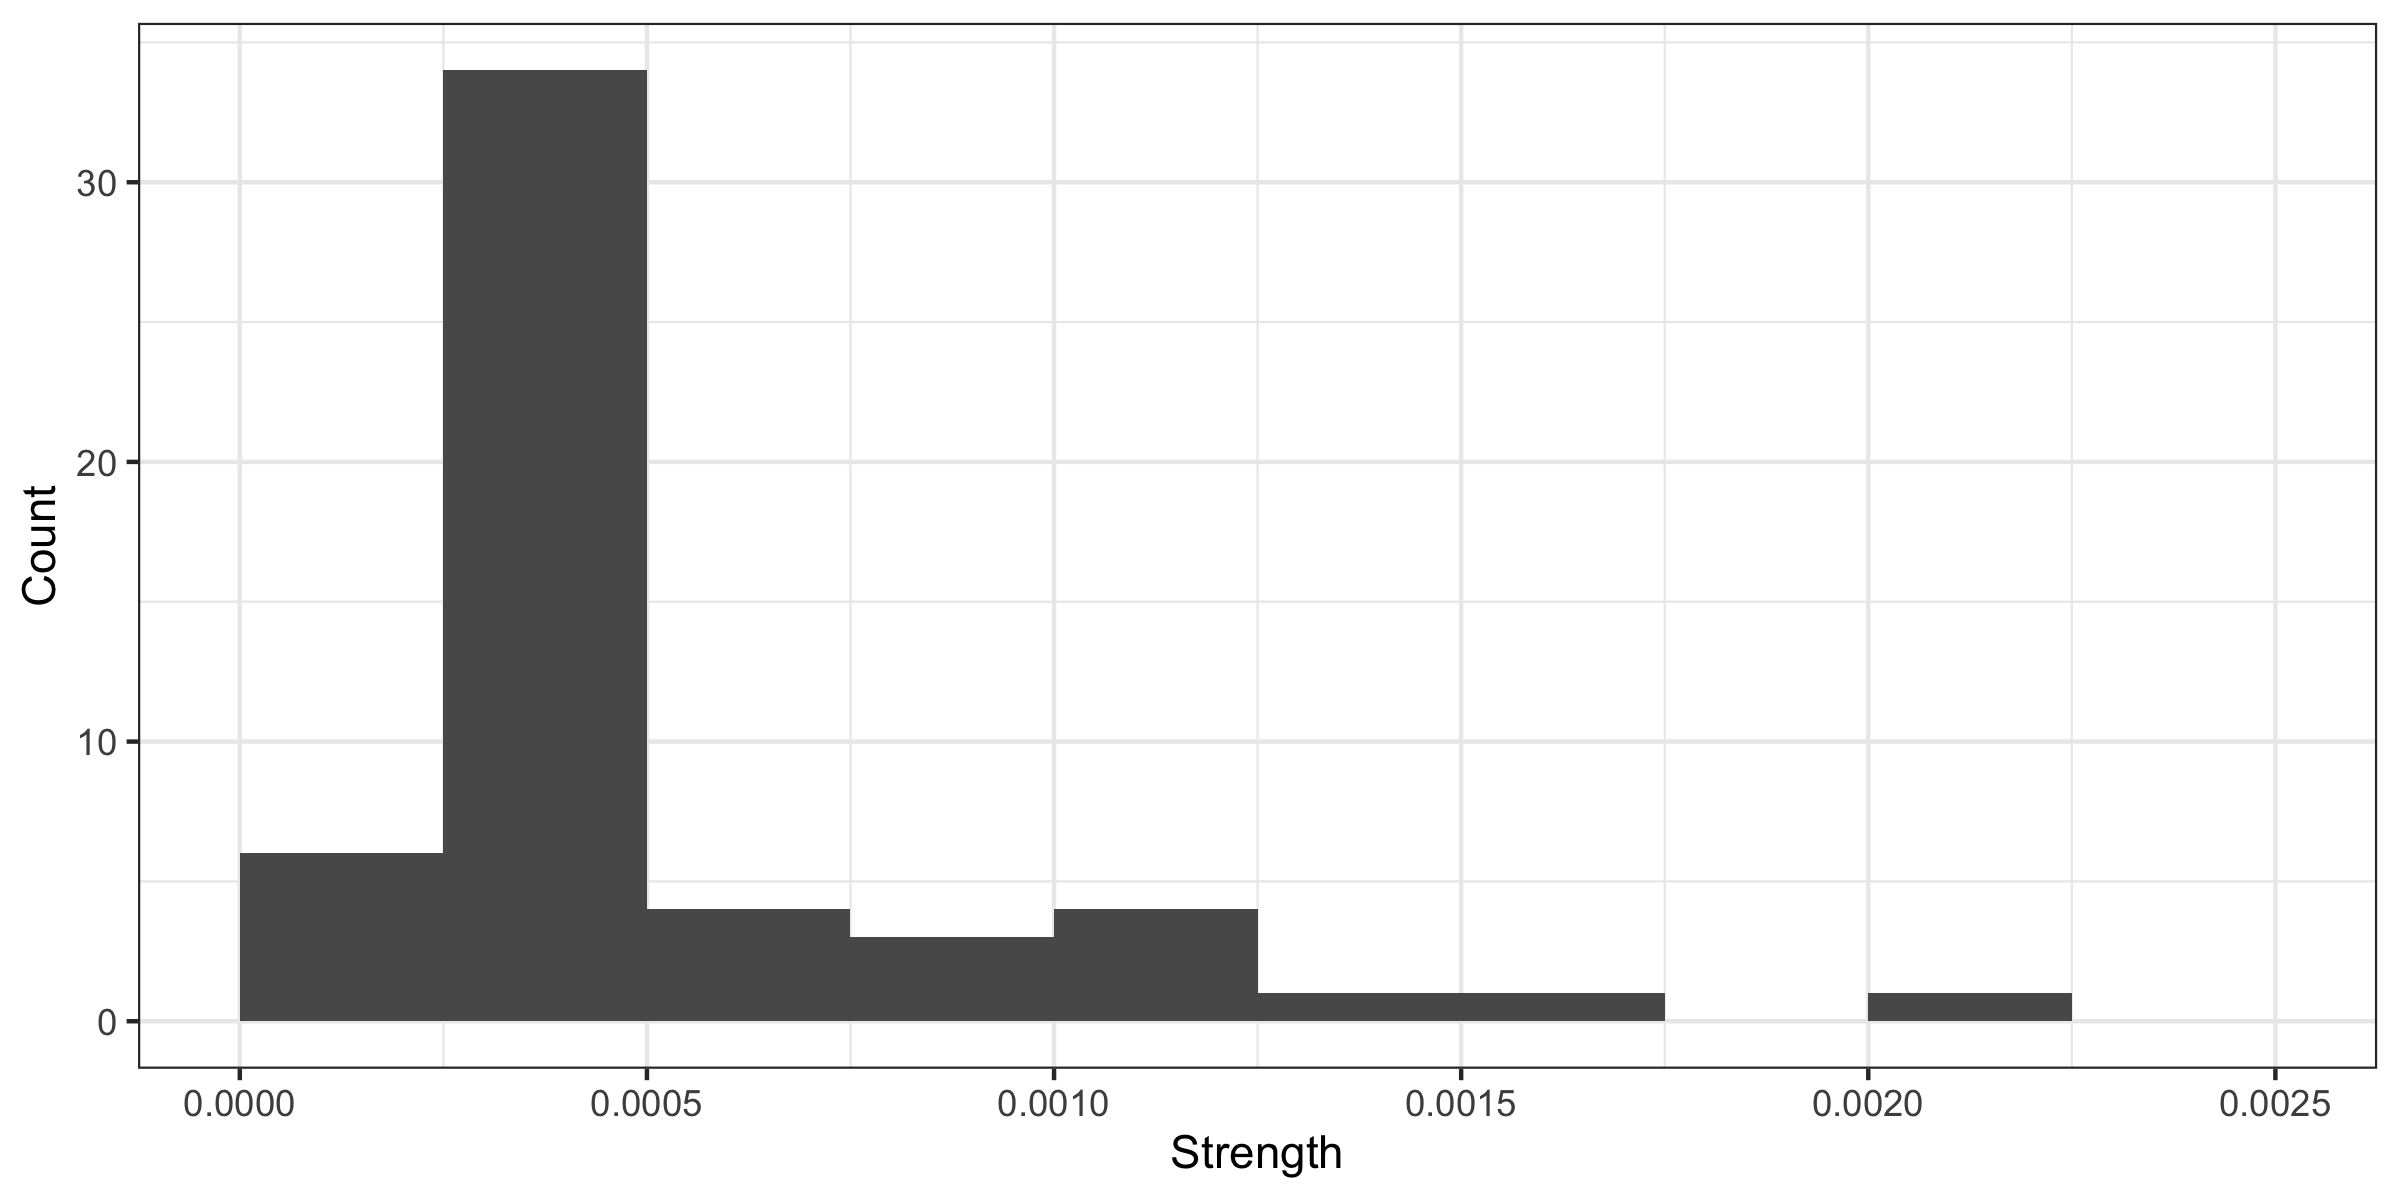
\includegraphics[width = 0.99\linewidth]{/Users/ralphtrane/Documents/RPackages_dev/ACEBounds/figures/example_analyses/cholesterol_heart_attack_strength_histogram.png}
 \caption{Histogram of strengths of IVs on the exposure. Here, SNPs are IVs, and high cholesterol is the exposure. We see that all IVs are very weak, with the largest value below 0.00225.}
 \label{fig:cholesterol_heart_attack_strength_histogram}
\end{figure}

\begin{figure}[H]
  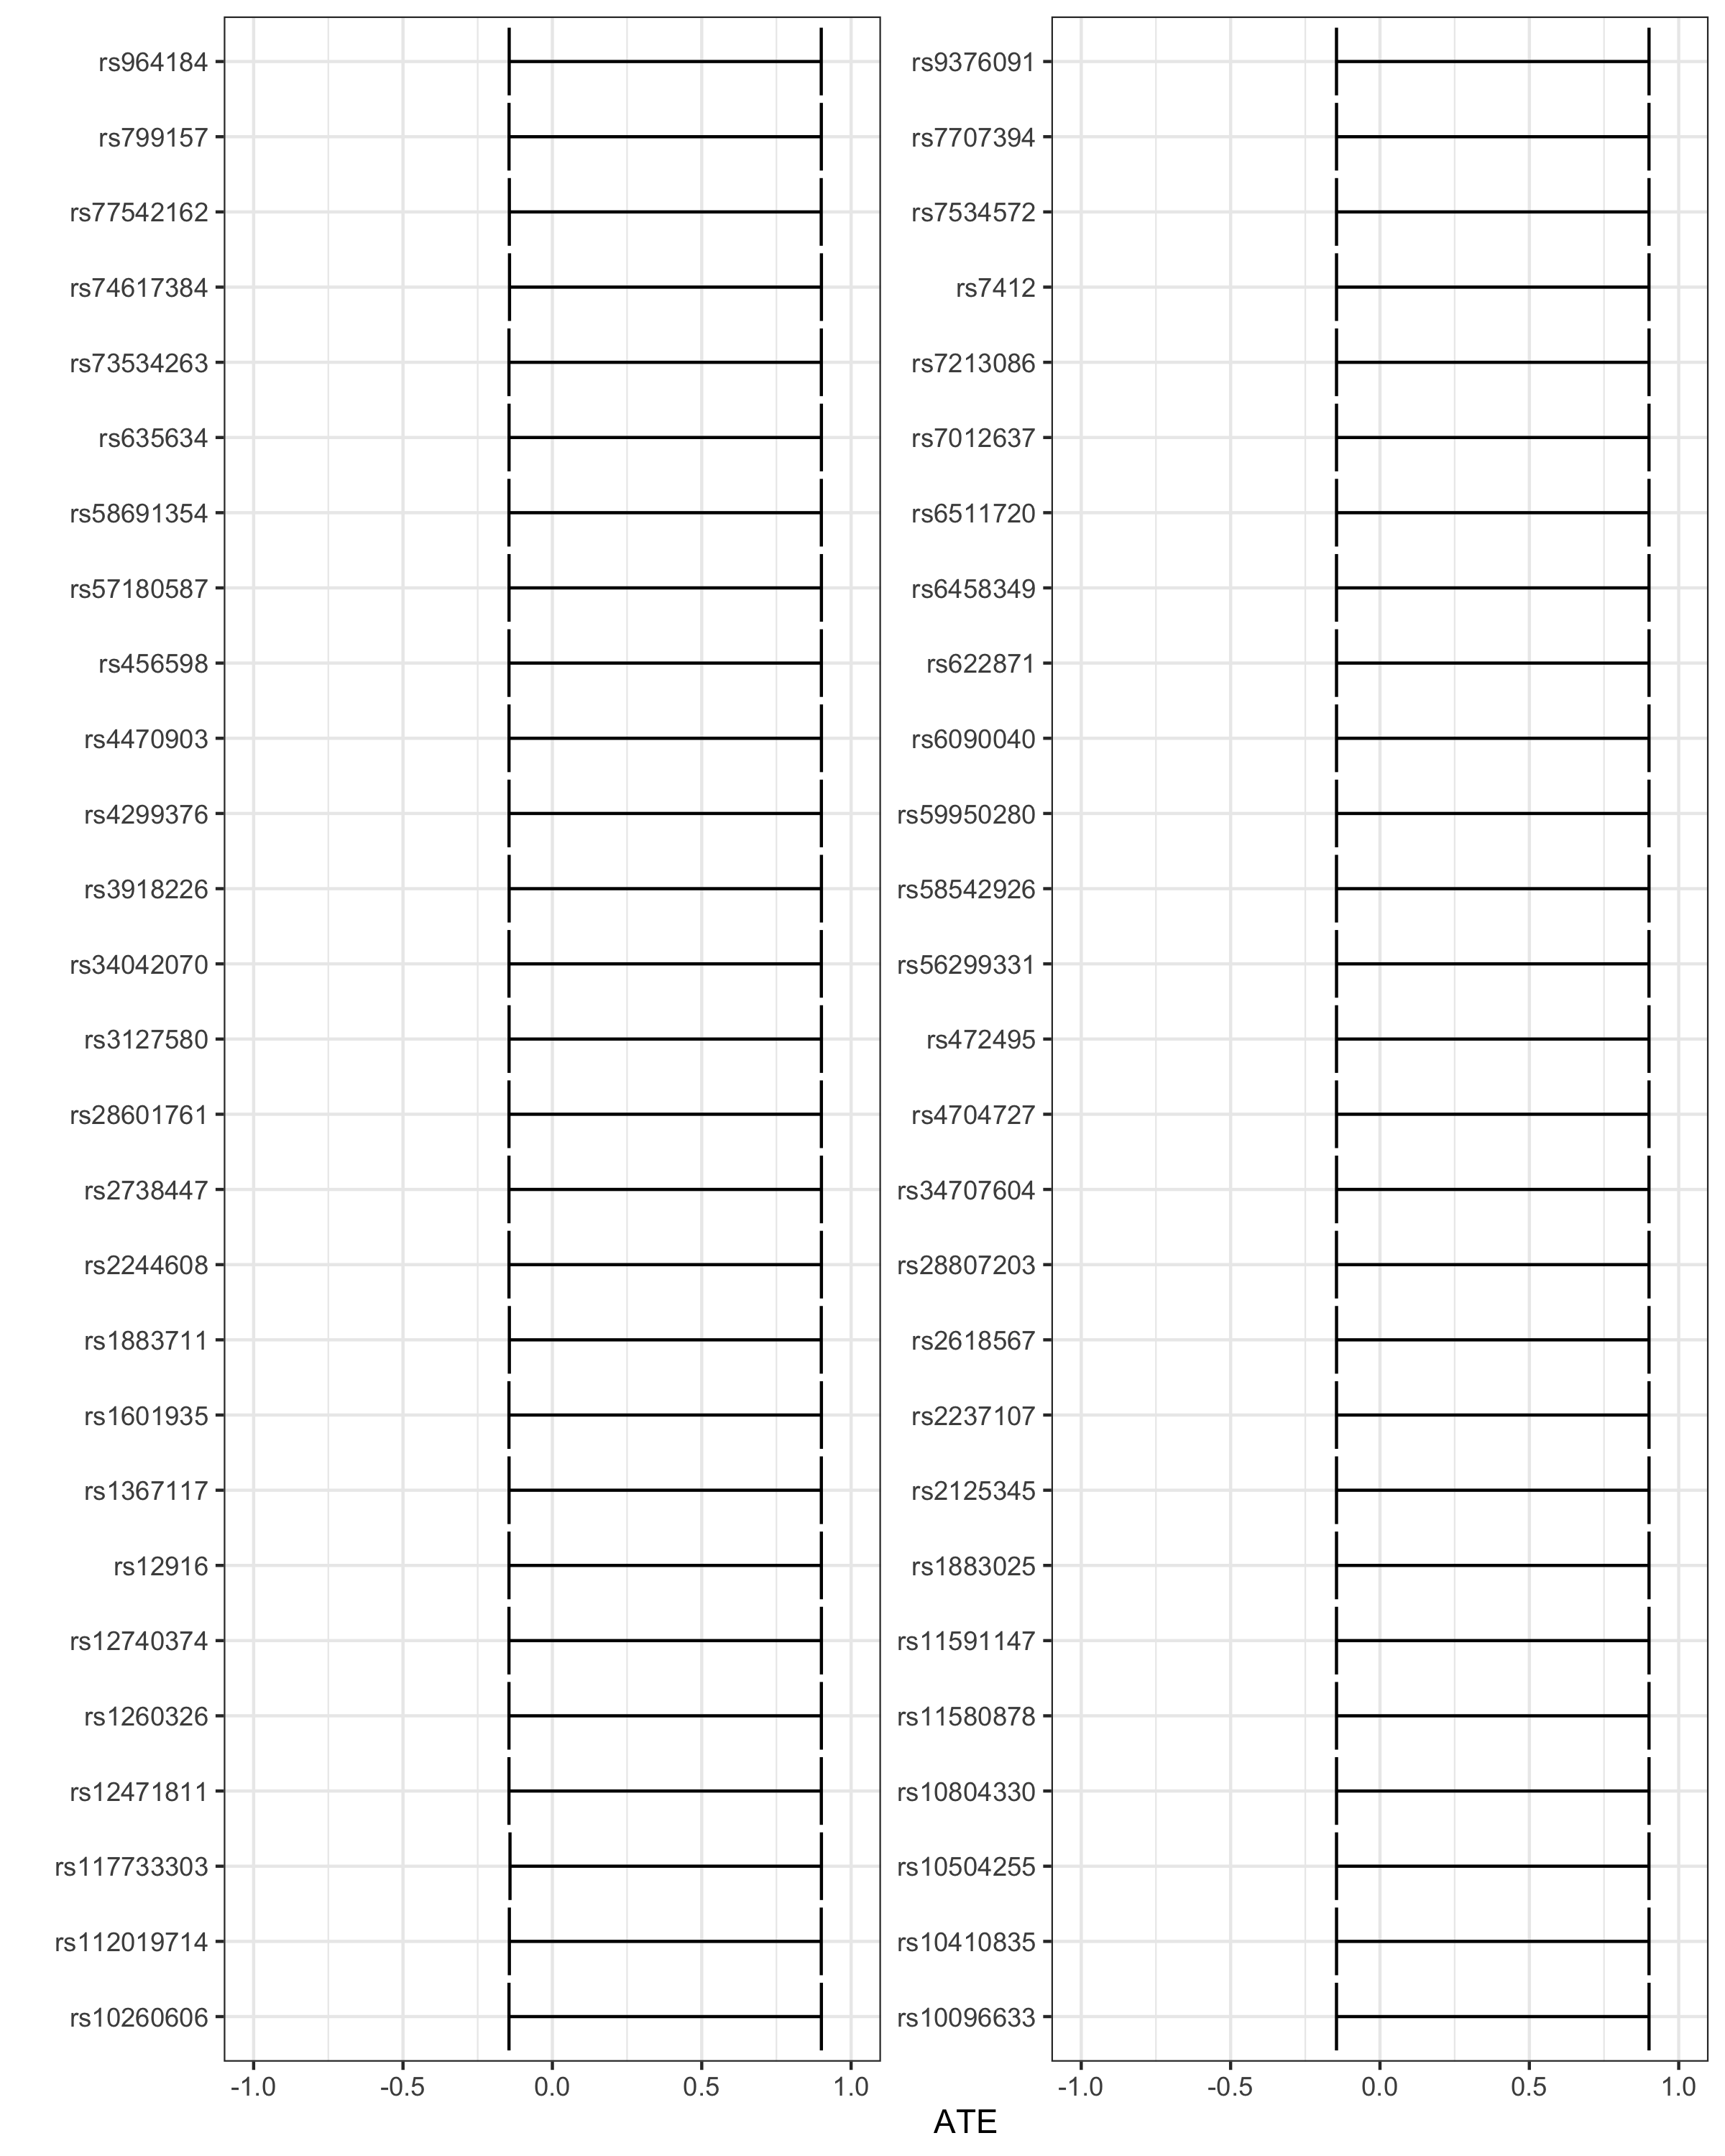
\includegraphics[width = 0.99\linewidth]{/Users/ralphtrane/Documents/RPackages_dev/ACEBounds/figures/example_analyses/cholesterol_heart_attack_bivaraite_bounds_ukb-a-108_ukb-a-434.png}
  \caption{Nonparametric two-sample IV bounds on the average treatment effect of high cholesterol on the incidence of heart attack.}
  \label{fig:cholesterol_on_heart_attack_ind_bounds}
\end{figure}

\begin{figure}[H]
  \center
  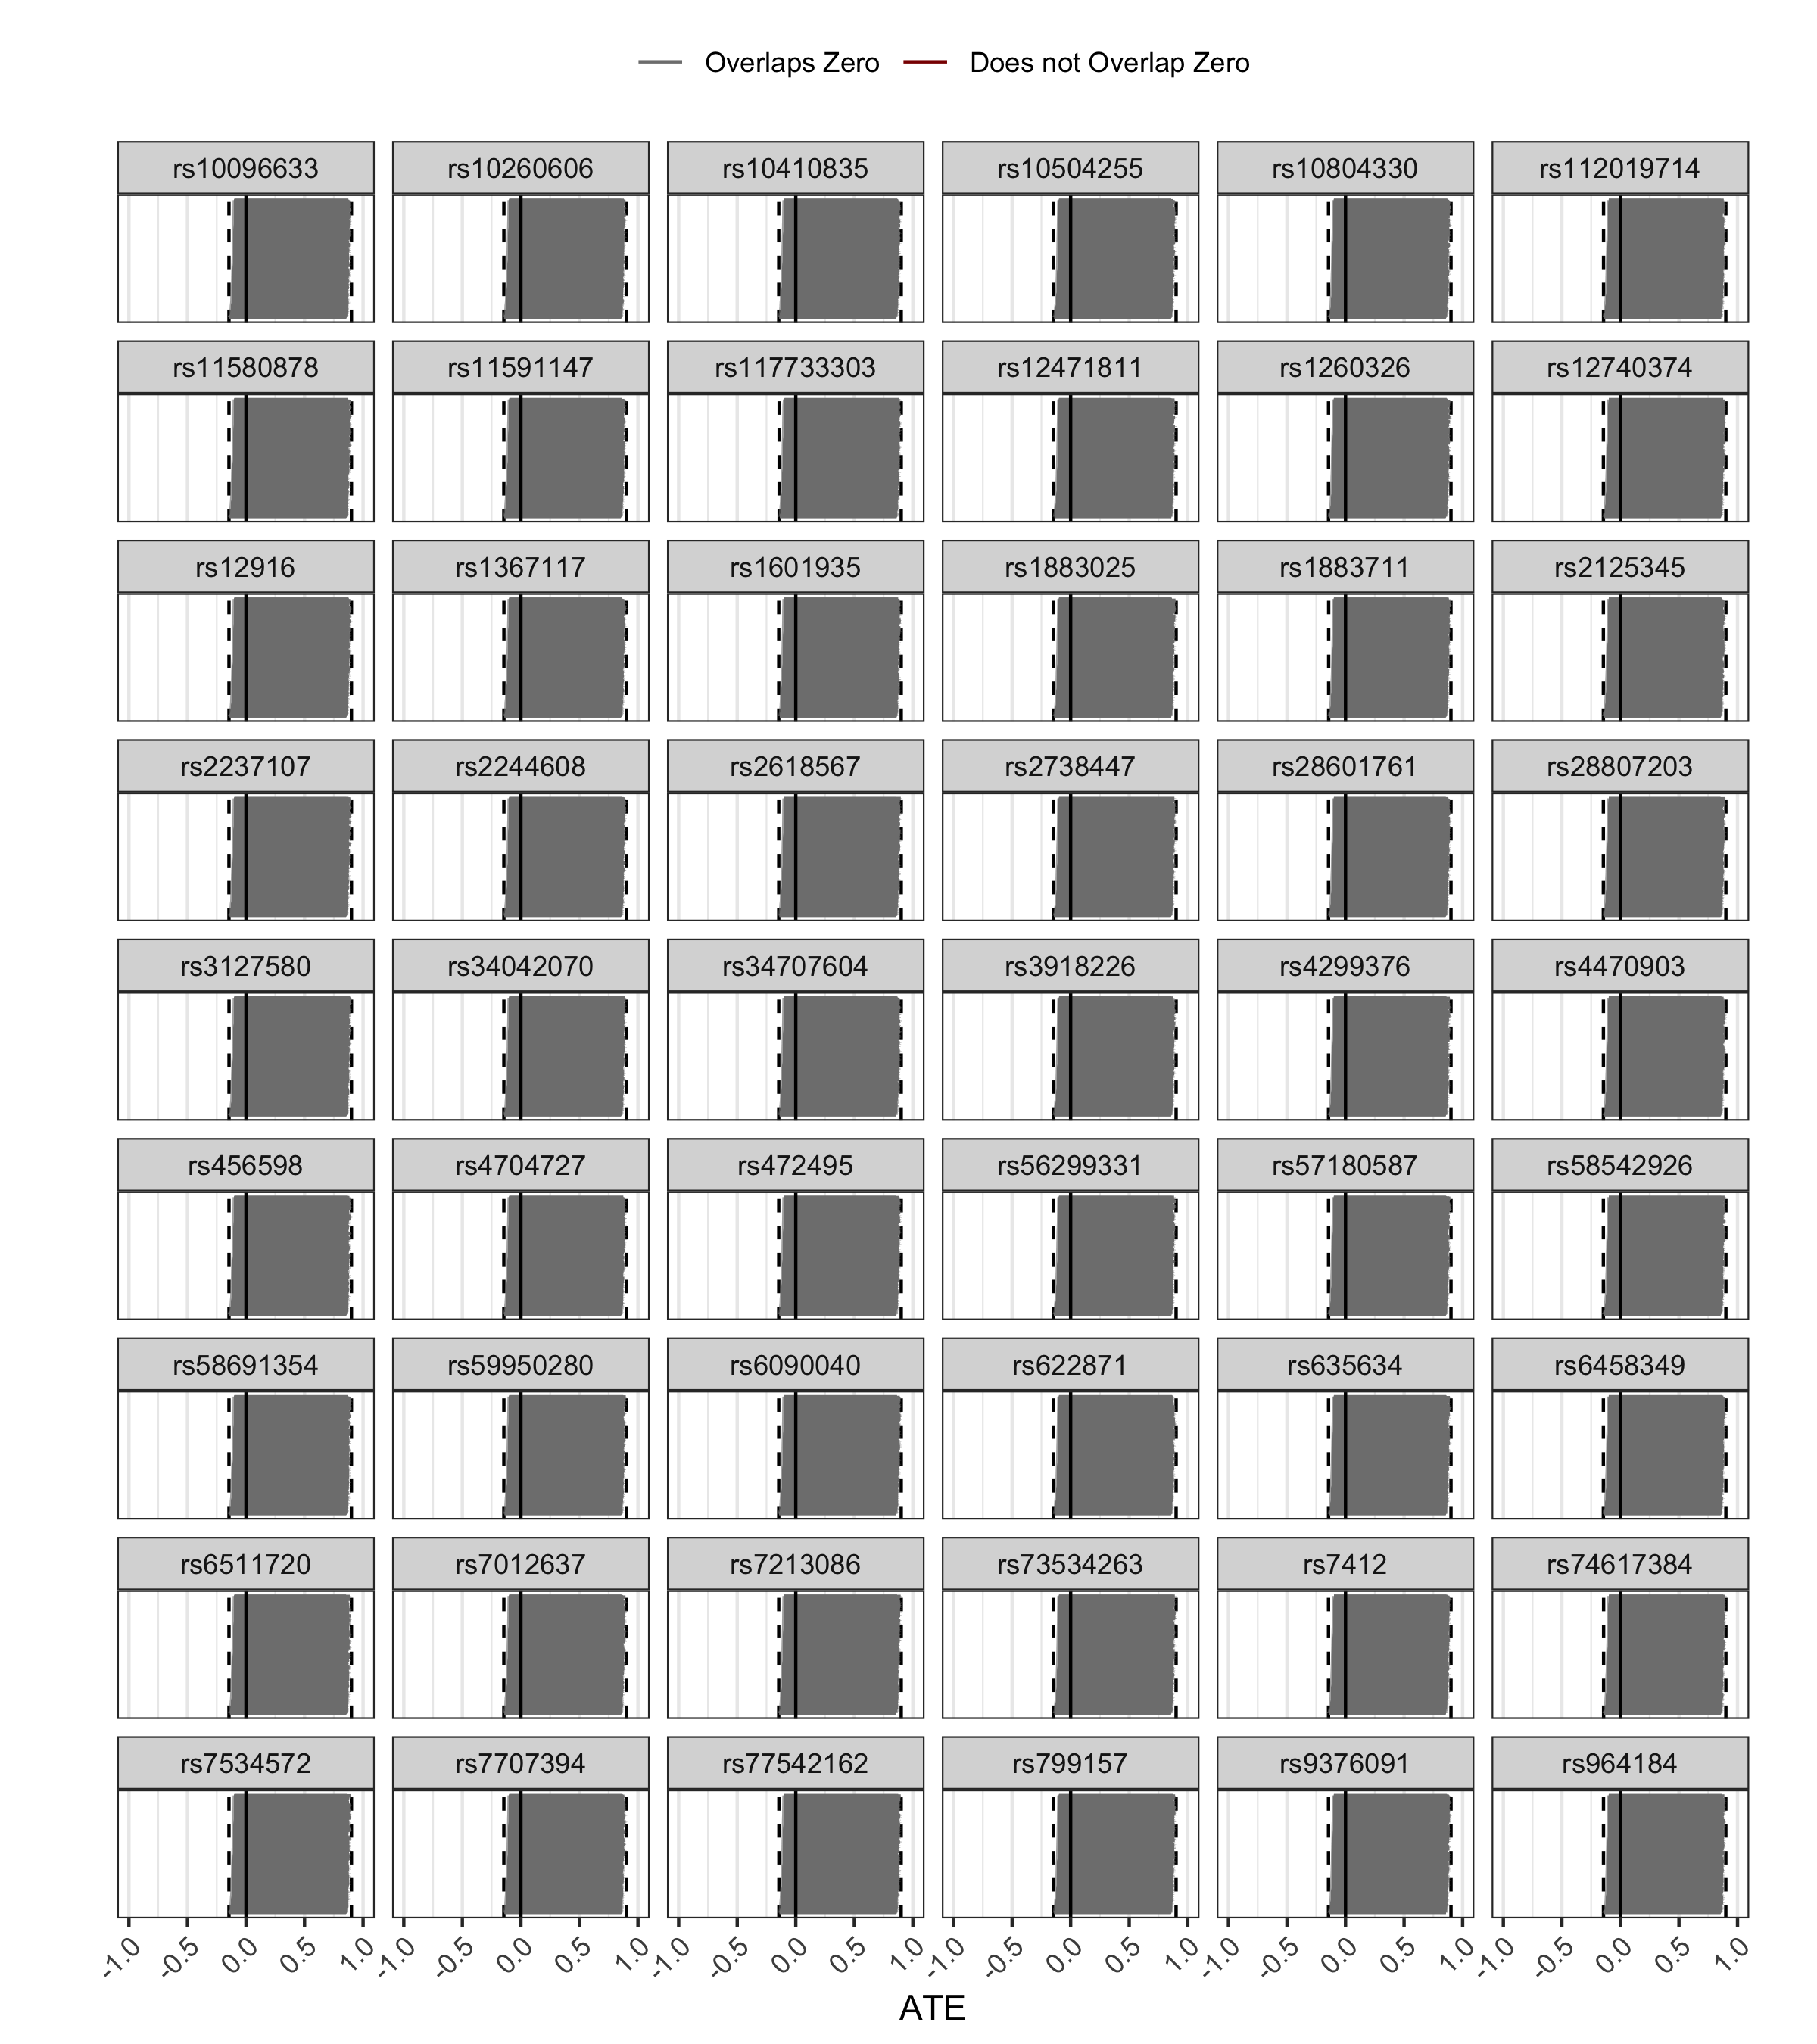
\includegraphics[width = 0.99\textwidth]{/Users/ralphtrane/Documents/RPackages_dev/ACEBounds/figures/example_analyses/cholesterol_heart_attack_individual_SNPs_plot_ukb-a-108_ukb-a-434.png}
    \caption{500 sets of bounds of the average treatment effect of high cholesterol on heart attack for each of the 54 SNPs. Each bound is based on a set of values for the trivariate distribution randomly sampled. Bounds are color coded to show if they overlap 0 (grey) or do not (red). All bounds overlap 0.}
    \label{fig:cholesterol_heart_attack_tri_bounds_all}
\end{figure}

\begin{figure}[H]
  \center
  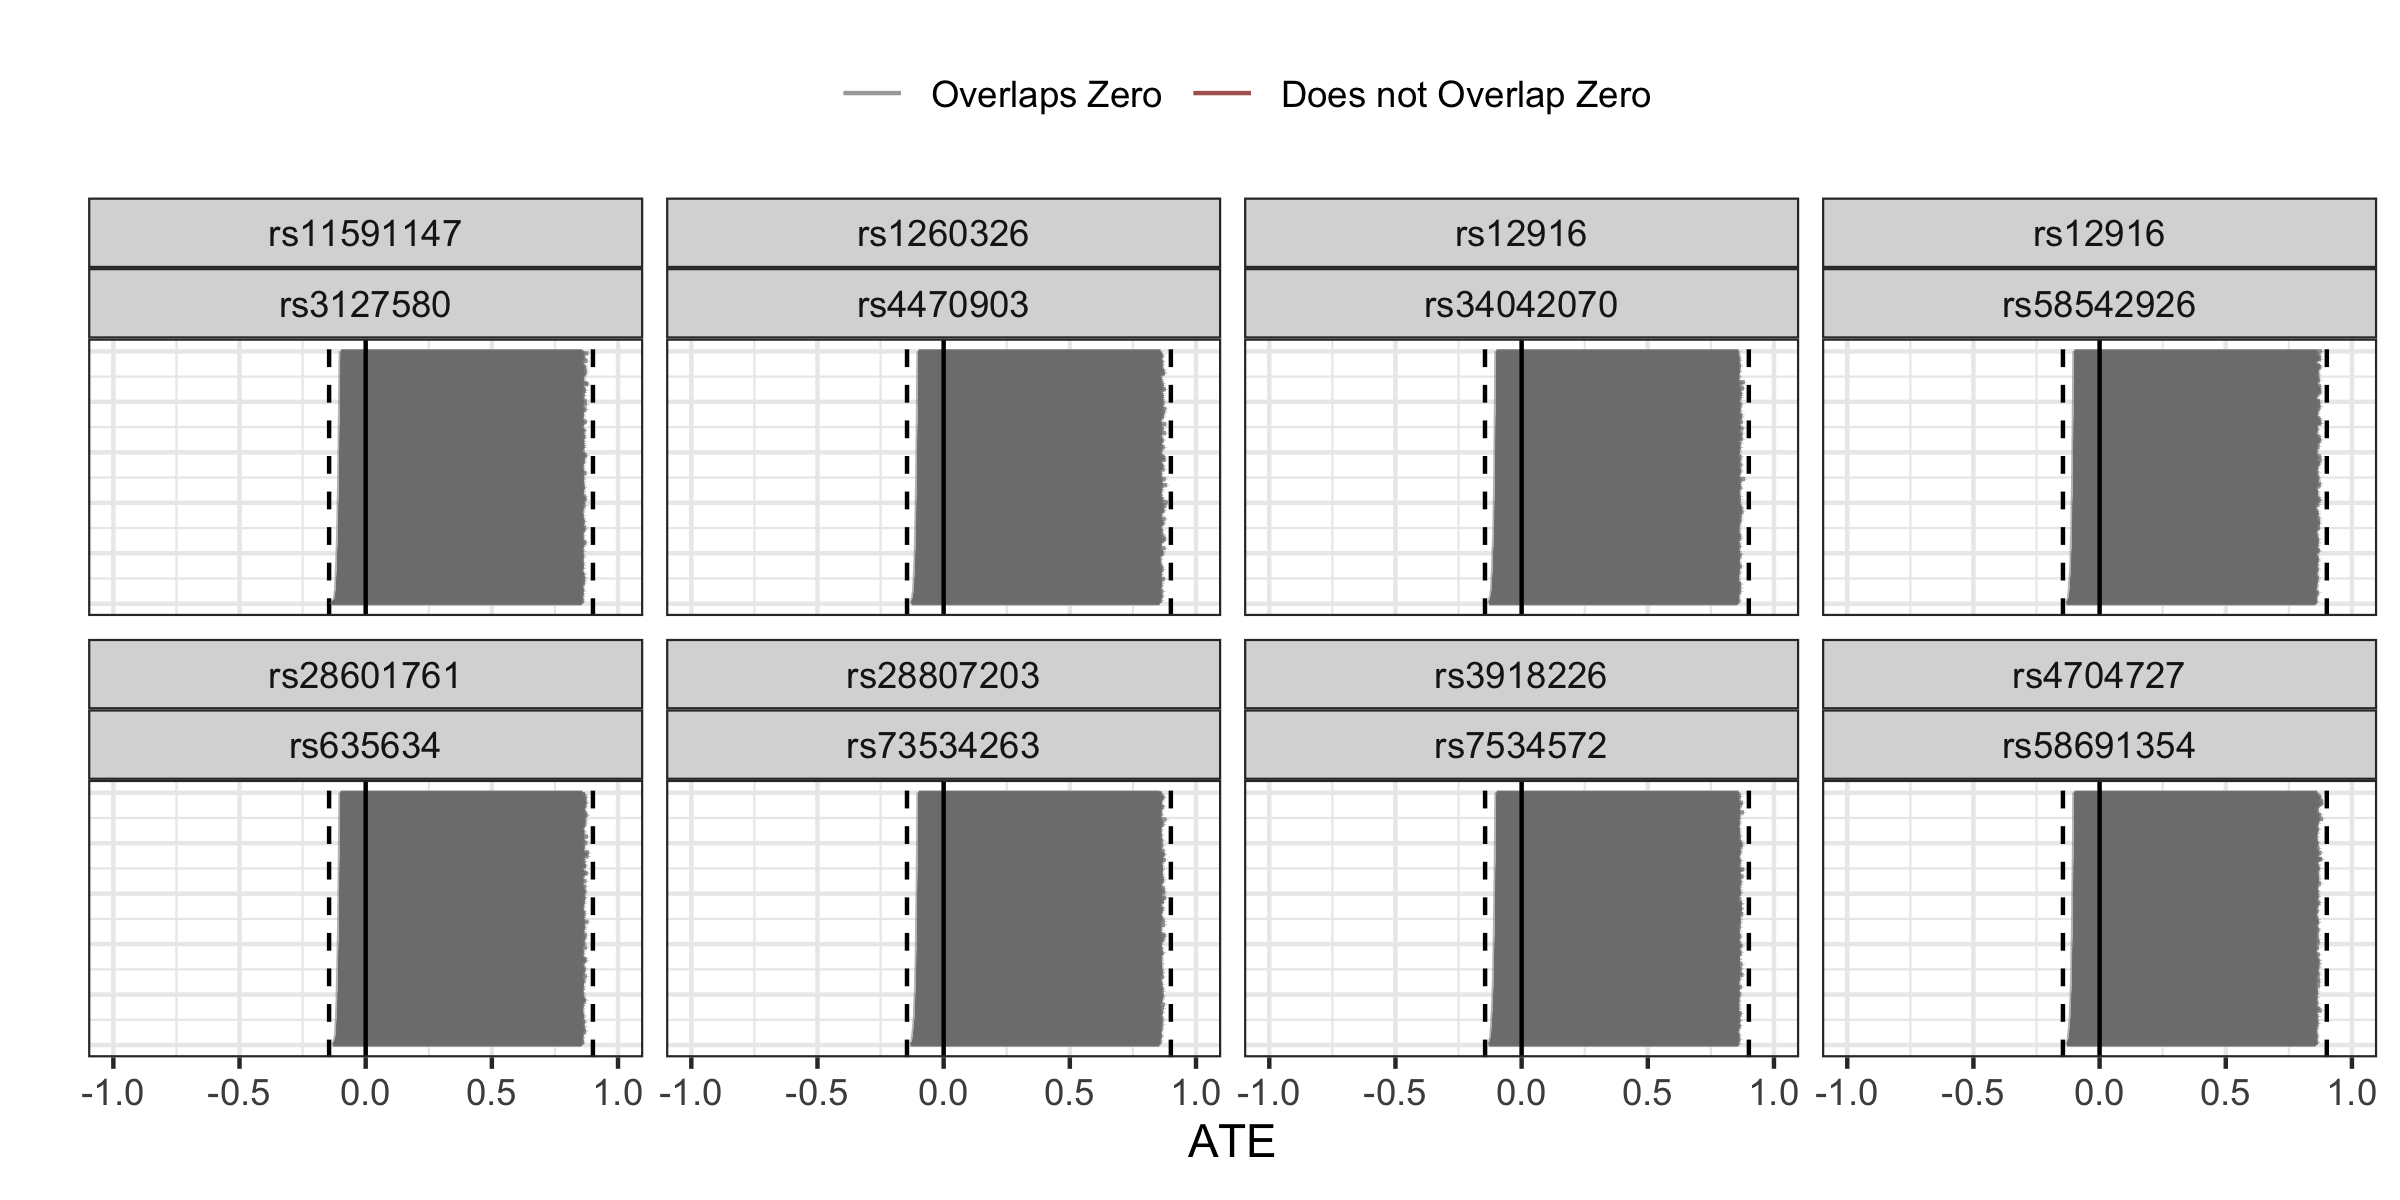
\includegraphics[width = 0.99\linewidth]{/Users/ralphtrane/Documents/RPackages_dev/ACEBounds/figures/example_analyses/cholesterol_heart_attack_intersection_bounds_plot_ukb-a-108_ukb-a-434.png}
  \caption{Intersection bounds of the average treatment effect of high cholesterol on heart attack based on randomly sampled trivariate distributions from pairs of SNPs. These 8 pairs were randomly chosen from all possible pairs.}
  \label{fig:cholesterol_on_heart_attack_intersections}
\end{figure}

\printbibliography[title=References]

\end{document}
